%%%%%%%%%%%%%%%%%%%%%%%%%%%%%%%%%%%%%%%%%
% The Legrand Orange Book
% LaTeX Template
% Version 2.4 (26/09/2018)
%
% This template was downloaded from:
% http://www.LaTeXTemplates.com
%
% Original author:
% Mathias Legrand (legrand.mathias@gmail.com) with modifications by:
% Vel (vel@latextemplates.com)
%
% License:
% CC BY-NC-SA 3.0 (http://creativecommons.org/licenses/by-nc-sa/3.0/)
%
% Compiling this template:
% This template uses biber for its bibliography and makeindex for its index.
% When you first open the template, compile it from the command line with the 
% commands below to make sure your LaTeX distribution is configured correctly:
%
% 1) pdflatex main
% 2) makeindex main.idx -s StyleInd.ist
% 3) biber main
% 4) pdflatex main x 2
%
% After this, when you wish to update the bibliography/index use the appropriate
% command above and make sure to compile with pdflatex several times 
% afterwards to propagate your changes to the document.
%
% This template also uses a number of packages which may need to be
% updated to the newest versions for the template to compile. It is strongly
% recommended you update your LaTeX distribution if you have any
% compilation errors.
%
% Important note:
% Chapter heading images should have a 2:1 width:height ratio,
% e.g. 920px width and 460px height.
%
%%%%%%%%%%%%%%%%%%%%%%%%%%%%%%%%%%%%%%%%%

%----------------------------------------------------------------------------------------
%	PACKAGES AND OTHER DOCUMENT CONFIGURATIONS
%----------------------------------------------------------------------------------------

\documentclass[11pt,fleqn,dvipsnames]{book} % Default font size and left-justified equations
\usepackage[dvipsnames]{xcolor}
\usepackage{tikz}
\usepackage{graphicx}
\usetikzlibrary{arrows,automata,positioning,trees,shadows}

\usepackage[font=small]{caption}
\usepackage{listings}
\usepackage{clrscode3e}
\usepackage[final]{pdfpages}
\usepackage{scrextend}
\usepackage{vwcol}

% Packages to enable extra letters and symbols
\usepackage{upgreek}

%%%%%%%%%%%%%%%%%%%%%%%%%%%%%%%%%%%%%%%%%
% The Legrand Orange Book
% Structural Definitions File
% Version 2.1 (26/09/2018)
%
% Original author:
% Mathias Legrand (legrand.mathias@gmail.com) with modifications by:
% Vel (vel@latextemplates.com)
% 
% This file was downloaded from:
% http://www.LaTeXTemplates.com
%
% License:
% CC BY-NC-SA 3.0 (http://creativecommons.org/licenses/by-nc-sa/3.0/)
%
%%%%%%%%%%%%%%%%%%%%%%%%%%%%%%%%%%%%%%%%%

%----------------------------------------------------------------------------------------
%	VARIOUS REQUIRED PACKAGES AND CONFIGURATIONS
%----------------------------------------------------------------------------------------

\usepackage[dvipsnames]{xcolor} % Required for specifying colors by name

\usepackage{graphicx} % Required for including pictures
\graphicspath{{figures/}} % Specifies the directory where pictures are stored
\usepackage{subfig}
\usepackage{graphbox}

\usepackage{lipsum} % Inserts dummy text
\usepackage{pifont} % Symbols

\newcommand{\cmark}{\ding{51}}
\newcommand{\xmark}{\ding{55}}

\usepackage{tikz} % Required for drawing custom shapes
\usepackage{tikzpagenodes}
\usetikzlibrary{calc}

\usepackage[english]{babel} % English language/hyphenation

\usepackage{enumitem} % Customize lists
\setlist{nolistsep} % Reduce spacing between bullet points and numbered lists

\usepackage{booktabs} % Required for nicer horizontal rules in tables
\usepackage{multirow}

\definecolor{ocre}{HTML}{24B3A8}
\definecolor{seagreen}{rgb}{0.18, 0.55, 0.34}
\definecolor{tut}{HTML}{4c9d4c}
\definecolor{good_green}{HTML}{00b294}
\definecolor{bad_red}{HTML}{a80000}
\definecolor{pitfall_orange}{HTML}{ff8c00}

%----------------------------------------------------------------------------------------
%	MARGINS
%----------------------------------------------------------------------------------------

\usepackage{geometry} % Required for adjusting page dimensions and margins

\geometry{
	paper=letterpaper, % Paper size, change to letterpaper for US letter size
	top=3cm, % Top margin
	bottom=3cm, % Bottom margin
	left=3cm, % Left margin
	right=3cm, % Right margin
	headheight=3cm, % Header height
	footskip=1.4cm, % Space from the bottom margin to the baseline of the footer
	headsep=10pt, % Space from the top margin to the baseline of the header
	%showframe, % Uncomment to show how the type block is set on the page
}

%----------------------------------------------------------------------------------------
%	FONTS
%----------------------------------------------------------------------------------------

\usepackage{avant} % Use the Avantgarde font for headings
%\usepackage{times} % Use the Times font for headings
\usepackage{mathptmx} % Use the Adobe Times Roman as the default text font together with math symbols from the Symbol, Chancery and Computer Modern fonts
\DeclareMathAlphabet{\mathcal}{OMS}{cmsy}{m}{n}
\DeclareSymbolFont{symbols}{OMS}{cmsy}{m}{n}
\DeclareSymbolFont{largesymbols}{OMX}{cmex}{m}{n}
\usepackage{microtype} % Slightly tweak font spacing for aesthetics
\usepackage[utf8]{inputenc} % Required for including letters with accents
\usepackage[T1]{fontenc} % Use 8-bit encoding that has 256 glyphs

%----------------------------------------------------------------------------------------
%	BIBLIOGRAPHY AND INDEX
%----------------------------------------------------------------------------------------

\usepackage[style=numeric,citestyle=numeric,sorting=nyt,sortcites=true,autopunct=true,babel=hyphen,hyperref=true,abbreviate=false,backref=true,backend=biber]{biblatex}
\nocite{*}
\addbibresource{bibliography.bib} % BibTeX bibliography file
\defbibheading{bibempty}{}

\usepackage{calc} % For simpler calculation - used for spacing the index letter headings correctly
\usepackage{makeidx} % Required to make an index
\makeindex % Tells LaTeX to create the files required for indexing

%----------------------------------------------------------------------------------------
%	MAIN TABLE OF CONTENTS
%----------------------------------------------------------------------------------------

\usepackage{titletoc} % Required for manipulating the table of contents

\contentsmargin{0cm} % Removes the default margin

% Part text styling (this is mostly taken care of in the PART HEADINGS section of this file)
\titlecontents{part}
	[0cm] % Left indentation
	{\addvspace{20pt}\bfseries} % Spacing and font options for parts
	{}
	{}
	{}

% Chapter text styling
\titlecontents{chapter}
	[1.25cm] % Left indentation
	{\addvspace{12pt}\large\sffamily\bfseries} % Spacing and font options for chapters
	{\color{ocre!60}\contentslabel[\Large\thecontentslabel]{1.25cm}\color{ocre}} % Formatting of numbered sections of this type
	{\color{ocre}} % Formatting of numberless sections of this type
	{\color{ocre!60}\normalsize\;\titlerule*[.5pc]{.}\;\thecontentspage} % Formatting of the filler to the right of the heading and the page number

% Section text styling
\titlecontents{section}
	[1.25cm] % Left indentation
	{\addvspace{3pt}\sffamily\bfseries} % Spacing and font options for sections
	{\contentslabel[\thecontentslabel]{1.25cm}} % Formatting of numbered sections of this type
	{} % Formatting of numberless sections of this type
	{\hfill\color{black}\thecontentspage} % Formatting of the filler to the right of the heading and the page number

% Subsection text styling
\titlecontents{subsection}
	[1.25cm] % Left indentation
	{\addvspace{1pt}\sffamily\small} % Spacing and font options for subsections
	{\contentslabel[\thecontentslabel]{1.25cm}} % Formatting of numbered sections of this type
	{} % Formatting of numberless sections of this type
	{\ \titlerule*[.5pc]{.}\;\thecontentspage} % Formatting of the filler to the right of the heading and the page number

% Figure text styling
\titlecontents{figure}
	[1.25cm] % Left indentation
	{\addvspace{1pt}\sffamily\small} % Spacing and font options for figures
	{\thecontentslabel\hspace*{1em}} % Formatting of numbered sections of this type
	{} % Formatting of numberless sections of this type
	{\ \titlerule*[.5pc]{.}\;\thecontentspage} % Formatting of the filler to the right of the heading and the page number

% Table text styling
\titlecontents{table}
	[1.25cm] % Left indentation
	{\addvspace{1pt}\sffamily\small} % Spacing and font options for tables
	{\thecontentslabel\hspace*{1em}} % Formatting of numbered sections of this type
	{} % Formatting of numberless sections of this type
	{\ \titlerule*[.5pc]{.}\;\thecontentspage} % Formatting of the filler to the right of the heading and the page number

%----------------------------------------------------------------------------------------
%	MINI TABLE OF CONTENTS IN PART HEADS
%----------------------------------------------------------------------------------------

% Chapter text styling
\titlecontents{lchapter}
	[0em] % Left indentation
	{\addvspace{15pt}\large\sffamily\bfseries} % Spacing and font options for chapters
	{\color{ocre}\contentslabel[\Large\thecontentslabel]{1.25cm}\color{ocre}} % Chapter number
	{}  
	{\color{ocre}\normalsize\sffamily\bfseries\;\titlerule*[.5pc]{.}\;\thecontentspage} % Page number

% Section text styling
\titlecontents{lsection}
	[0em] % Left indentation
	{\sffamily\small} % Spacing and font options for sections
	{\contentslabel[\thecontentslabel]{1.25cm}} % Section number
	{}
	{}

% Subsection text styling (note these aren't shown by default, display them by searchings this file for tocdepth and reading the commented text)
\titlecontents{lsubsection}
	[.5em] % Left indentation
	{\sffamily\footnotesize} % Spacing and font options for subsections
	{\contentslabel[\thecontentslabel]{1.25cm}}
	{}
	{}

%----------------------------------------------------------------------------------------
%	HEADERS AND FOOTERS
%----------------------------------------------------------------------------------------

\usepackage{fancyhdr} % Required for header and footer configuration

\pagestyle{fancy} % Enable the custom headers and footers

\renewcommand{\chaptermark}[1]{\markboth{\sffamily\normalsize\bfseries\thechapter.\ #1}{A}} % Styling for the current chapter in the header
\renewcommand{\sectionmark}[1]{\markright{\sffamily\normalsize\thesection\hspace{5pt}#1}{}} % Styling for the current section in the header

\fancyhf{} % Clear default headers and footers

\fancyhead[E]{
    \begin{tikzpicture}[overlay, remember picture]%
        \fill[ocre] (current page.north west) rectangle ($(current page.north east)+(0,-.5in)$);
        \node[anchor=north west, text=white, minimum size=.5in, inner xsep=5mm] at (current page.north west) {\sffamily\normalsize\thepage};
        \node[anchor=north east, text=white, minimum size=.5in, inner xsep=5mm] at (current page.north east) {\leftmark};
    \end{tikzpicture}
}

\fancyhead[O]{
    \begin{tikzpicture}[overlay, remember picture]%
        \fill[ocre] (current page.north west) rectangle ($(current page.north east)+(0,-.5in)$);
        \node[anchor=north east, text=white, minimum size=.5in, inner xsep=5mm] at (current page.north east) {\sffamily\normalsize\thepage};
        \node[anchor=north west, text=white, minimum size=.5in, inner xsep=5mm] at (current page.north west) {\leftmark};
    \end{tikzpicture}
}

%\fancyhead[LE,RO]{\sffamily\normalsize\thepage} % Styling for the page number in the header
%\fancyhead[LO]{\rightmark} % Print the nearest section name on the left side of odd pages
%\fancyhead[RE]{\leftmark} % Print the current chapter name on the right side of even pages
%\fancyfoot[C]{\thepage} % Uncomment to include a footer

\renewcommand{\headrulewidth}{0pt} % Thickness of the rule under the header

\fancypagestyle{plain}{% Style for when a plain pagestyle is specified
	\fancyhead{}\renewcommand{\headrulewidth}{0pt}%
}

% Removes the header from odd empty pages at the end of chapters
\makeatletter
\renewcommand{\cleardoublepage}{
\clearpage\ifodd\c@page\else
\hbox{}
\vspace*{\fill}
\thispagestyle{empty}
\newpage
\fi}

%----------------------------------------------------------------------------------------
%	THEOREM STYLES
%----------------------------------------------------------------------------------------

\usepackage{amsmath,amsfonts,amssymb,amsthm} % For math equations, theorems, symbols, etc

\newcommand{\intoo}[2]{\mathopen{]}#1\,;#2\mathclose{[}}
\newcommand{\ud}{\mathop{\mathrm{{}d}}\mathopen{}}
\newcommand{\intff}[2]{\mathopen{[}#1\,;#2\mathclose{]}}
\renewcommand{\qedsymbol}{$\blacksquare$}
\newtheorem{notation}{Notation}[chapter]

% Boxed/framed environments
\newtheoremstyle{ocrenumbox}% Theorem style name
{0pt}% Space above
{0pt}% Space below
{\normalfont}% Body font
{}% Indent amount
{\small\bf\sffamily\color{ocre}}% Theorem head font
{\;}% Punctuation after theorem head
{0.25em}% Space after theorem head
{\small\sffamily\color{ocre}\thmname{#1}\nobreakspace\thmnumber{\@ifnotempty{#1}{}\@upn{#2}}% Theorem text (e.g. Theorem 2.1)
\thmnote{\nobreakspace\the\thm@notefont\sffamily\bfseries\color{black}---\nobreakspace#3.}} % Optional theorem note

\newtheoremstyle{blacknumex}% Theorem style name
{5pt}% Space above
{5pt}% Space below
{\normalfont}% Body font
{} % Indent amount
{\small\bf\sffamily}% Theorem head font
{\;}% Punctuation after theorem head
{0.25em}% Space after theorem head
{\small\sffamily{\tiny\ensuremath{\blacksquare}}\nobreakspace\thmname{#1}\nobreakspace\thmnumber{\@ifnotempty{#1}{}\@upn{#2}}% Theorem text (e.g. Theorem 2.1)
\thmnote{\nobreakspace\the\thm@notefont\sffamily\bfseries---\nobreakspace#3.}}% Optional theorem note

\newtheoremstyle{blacknumbox} % Theorem style name
{0pt}% Space above
{0pt}% Space below
{\normalfont}% Body font
{}% Indent amount
{\small\bf\sffamily}% Theorem head font
{\;}% Punctuation after theorem head
{0.25em}% Space after theorem head
{\small\sffamily\thmname{#1}\nobreakspace\thmnumber{\@ifnotempty{#1}{}\@upn{#2}}% Theorem text (e.g. Theorem 2.1)
\thmnote{\nobreakspace\the\thm@notefont\sffamily\bfseries---\nobreakspace#3.}}% Optional theorem note

\newtheoremstyle{pinknumbox} % Axiom box style
{0pt}% Space above
{0pt}% Space below
{\normalfont}% Body font
{}% Indent amount
{\small\bf\sffamily}% Theorem head font
{\;}% Punctuation after theorem head
{0.25em}% Space after theorem head
{\small\sffamily\color{magenta}\thmname{#1}\nobreakspace\thmnumber{\@ifnotempty{#1}{}\@upn{#2}}% Theorem text (e.g. Theorem 2.1)
\thmnote{\nobreakspace\the\thm@notefont\sffamily\bfseries---\nobreakspace#3.}}

\newtheoremstyle{greennumbox} % Axiom box style
{0pt}% Space above
{0pt}% Space below
{\normalfont}% Body font
{}% Indent amount
{\small\bf\sffamily}% Theorem head font
{\;}% Punctuation after theorem head
{0.25em}% Space after theorem head
{\small\sffamily\color{Green}\thmname{#1}\nobreakspace\thmnumber{\@ifnotempty{#1}{}\@upn{#2}}% Theorem text (e.g. Theorem 2.1)
\thmnote{\nobreakspace\the\thm@notefont\sffamily\bfseries---\nobreakspace#3.}}

% Non-boxed/non-framed environments
\newtheoremstyle{ocrenum}% Theorem style name
{5pt}% Space above
{5pt}% Space below
{\normalfont}% Body font
{}% Indent amount
{\small\bf\sffamily\color{ocre}}% Theorem head font
{\;}% Punctuation after theorem head
{0.25em}% Space after theorem head
{\small\sffamily\color{ocre}\thmname{#1}\nobreakspace\thmnumber{\@ifnotempty{#1}{}\@upn{#2}}% Theorem text (e.g. Theorem 2.1)
\thmnote{\nobreakspace\the\thm@notefont\sffamily\bfseries\color{black}---\nobreakspace#3.}} % Optional theorem note
\makeatother

% Defines the theorem text style for each type of theorem to one of the three styles above
\newcounter{dummy} 
\numberwithin{dummy}{section}
\theoremstyle{ocrenumbox}
\newtheorem{theoremeT}[dummy]{Theorem}
\newtheorem{problem}{Problem}[chapter]
\newtheorem{exerciseT}{Exercise}[chapter]
\theoremstyle{blacknumex}
\newtheorem{exampleT}{Example}[chapter]
\theoremstyle{blacknumbox}
\newtheorem{vocabulary}{Vocabulary}[chapter]
\newtheorem{definitionT}{Definition}[section]
\newtheorem{corollaryT}[dummy]{Corollary}
\newtheorem{lemmaT}[dummy]{Lemma}
\theoremstyle{ocrenum}
\newtheorem{proposition}[dummy]{Proposition}
\theoremstyle{pinknumbox}
\newtheorem{axiomT}[dummy]{Axiom}
\theoremstyle{greennumbox}
\newtheorem{ruleT}{Template}[chapter]

% A new set of theorem definitions used in appendix only
\newcounter{appendixcounter}
\theoremstyle{greennumbox}
\newtheorem{ruleT_appendix}[appendixcounter]{Template}
\theoremstyle{pinknumbox}
\newtheorem{axiomT_appendix}[appendixcounter]{Axiom}
\theoremstyle{ocrenumbox}
\newtheorem{theoremeT_appendix}[appendixcounter]{Theorem}

%----------------------------------------------------------------------------------------
%	DEFINITION OF COLORED BOXES
%----------------------------------------------------------------------------------------

\RequirePackage[framemethod=default]{mdframed} % Required for creating the theorem, definition, exercise and corollary boxes

% Theorem box
\newmdenv[skipabove=1em,
skipbelow=7pt,
backgroundcolor=black!5,
linecolor=ocre,
innerleftmargin=5pt,
innerrightmargin=5pt,
innertopmargin=1.5em,
leftmargin=0cm,
rightmargin=0cm,
innerbottommargin=5pt]{tBox}

% Exercise box	  
\newmdenv[skipabove=1em,
skipbelow=7pt,
rightline=false,
leftline=true,
topline=false,
bottomline=false,
backgroundcolor=ocre!10,
linecolor=ocre,
innerleftmargin=5pt,
innerrightmargin=5pt,
innertopmargin=1em,
innerbottommargin=5pt,
leftmargin=0cm,
rightmargin=0cm,
linewidth=4pt]{eBox}	

% Definition box
\newmdenv[skipabove=1em,
skipbelow=7pt,
rightline=false,
leftline=true,
topline=false,
bottomline=false,
linecolor=ocre,
innerleftmargin=5pt,
innerrightmargin=5pt,
innertopmargin=1em,
leftmargin=0cm,
rightmargin=0cm,
linewidth=4pt,
innerbottommargin=0pt]{dBox}	

% Corollary box
\newmdenv[skipabove=1em,
skipbelow=7pt,
rightline=false,
leftline=true,
topline=false,
bottomline=false,
linecolor=gray,
backgroundcolor=black!5,
innerleftmargin=5pt,
innerrightmargin=5pt,
innertopmargin=1.5em,
leftmargin=0cm,
rightmargin=0cm,
linewidth=4pt,
innerbottommargin=5pt]{cBox}

% Axiom box
\newmdenv[skipabove=1em,
skipbelow=7pt,
rightline=false,
leftline=true,
topline=false,
bottomline=false,
linecolor=magenta,
backgroundcolor=magenta!5,
innerleftmargin=5pt,
innerrightmargin=5pt,
innertopmargin=1.5em,
leftmargin=0cm,
rightmargin=0cm,
linewidth=4pt,
innerbottommargin=5pt]{aBox}

% Rule box
\newmdenv[skipabove=1em,
skipbelow=7pt,
rightline=false,
leftline=true,
topline=false,
bottomline=false,
linecolor=Green,
backgroundcolor=Green!5,
innerleftmargin=5pt,
innerrightmargin=5pt,
innertopmargin=1.5em,
leftmargin=0cm,
rightmargin=0cm,
linewidth=4pt,
innerbottommargin=5pt]{rBox}

% Creates an environment for each type of theorem and assigns it a theorem text style from the "Theorem Styles" section above and a colored box from above
\newenvironment{theorem}{\begin{tBox}\begin{theoremeT}}{\end{theoremeT}\end{tBox}}
\newenvironment{exercise}{\begin{eBox}\begin{exerciseT}}{\hfill{\color{ocre}\tiny\ensuremath{\blacksquare}}\end{exerciseT}\end{eBox}}				  
\newenvironment{definition}{\begin{dBox}\begin{definitionT}}{\end{definitionT}\end{dBox}}	
\newenvironment{example}{\begin{exampleT}}{\hfill{\tiny\ensuremath{\blacksquare}}\end{exampleT}}		
\newenvironment{corollary}{\begin{cBox}\begin{corollaryT}}{\end{corollaryT}\end{cBox}}	
\newenvironment{lemma}{\begin{cBox}\begin{lemmaT}}{\end{lemmaT}\end{cBox}}	
\newenvironment{axiom}{\begin{aBox}\begin{axiomT}}{\end{axiomT}\end{aBox}}
\newenvironment{thmrule}{\begin{rBox}\begin{ruleT}}{\end{ruleT}\end{rBox}}

% A new set of environments for appendix only
\newenvironment{theorem_appendix}{\begin{tBox}\begin{theoremeT_appendix}}{\end{theoremeT_appendix}\end{tBox}}
\newenvironment{axiom_appendix}{\begin{aBox}\begin{axiomT_appendix}}{\end{axiomT_appendix}\end{aBox}}
\newenvironment{thmrule_appendix}{\begin{rBox}\begin{ruleT_appendix}}{\end{ruleT_appendix}\end{rBox}}

%----------------------------------------------------------------------------------------
%	REMARK ENVIRONMENT
%----------------------------------------------------------------------------------------

\newenvironment{remark}{\par\vspace{10pt}\small % Vertical white space above the remark and smaller font size
\begin{list}{}{
\leftmargin=35pt % Indentation on the left
\rightmargin=25pt}\item\ignorespaces % Indentation on the right
\makebox[-2.5pt]{\begin{tikzpicture}[overlay]
\node[draw=ocre!60,line width=1pt,circle,fill=ocre!25,font=\sffamily\bfseries,inner sep=2pt,outer sep=0pt] at (-15pt,0pt){\textcolor{ocre}{R}};\end{tikzpicture}} % R in a circle
\advance\baselineskip -1pt}{\end{list}\vskip5pt} % Tighter line spacing and white space after remark

\newenvironment{goodexample}{\vspace{5pt}\small % Vertical white space above the remark and smaller font size
\begin{list}{}{
\leftmargin=25pt % Indentation on the left
\rightmargin=25pt}\item\ignorespaces % Indentation on the right
\makebox[-2.5pt]{\begin{tikzpicture}[overlay]
\node[draw=good_green!60,line width=1pt,circle,fill=good_green!25,font=\sffamily\bfseries,inner sep=2pt,outer sep=0pt,minimum size=6mm] at (-15pt,0pt){\textcolor{good_green}{\cmark}};\end{tikzpicture}} % Checkmark in a circle
\advance\baselineskip -1pt}{\end{list}\vskip5pt}

\newenvironment{badexample}{\vspace{5pt}\small % Vertical white space above the remark and smaller font size
\begin{list}{}{
\leftmargin=25pt % Indentation on the left
\rightmargin=25pt}\item\ignorespaces % Indentation on the right
\makebox[-2.5pt]{\begin{tikzpicture}[overlay]
\node[draw=bad_red!60,line width=1pt,circle,fill=bad_red!25,font=\sffamily\bfseries,inner sep=2pt,outer sep=0pt,minimum size=6mm] at (-15pt,0pt){\textcolor{bad_red}{\xmark}};\end{tikzpicture}} % Crossmark in a circle
\advance\baselineskip -1pt}{\end{list}\vskip5pt}

\newenvironment{pitfall}{\vspace{5pt}\small % Vertical white space above the remark and smaller font size
\begin{list}{}{
\leftmargin=25pt % Indentation on the left
\rightmargin=25pt}\item\ignorespaces % Indentation on the right
\makebox[-2.5pt]{\begin{tikzpicture}[overlay]
\node[draw=pitfall_orange!60,line width=1pt,circle,fill=pitfall_orange!25,font=\sffamily\bfseries,inner sep=2pt,outer sep=0pt,minimum size=6mm] at (-15pt,0pt){\textcolor{pitfall_orange}{!}};\end{tikzpicture}} % ! in a circle
\advance\baselineskip -1pt}{\end{list}\vskip5pt}

%----------------------------------------------------------------------------------------
%	SECTION NUMBERING IN THE MARGIN
%----------------------------------------------------------------------------------------

\makeatletter
\renewcommand{\@seccntformat}[1]{\llap{\textcolor{ocre}{\csname the#1\endcsname}\hspace{1em}}}                    
\renewcommand{\section}{\@startsection{section}{1}{\z@}
{-4ex \@plus -1ex \@minus -.4ex}
{1ex \@plus.2ex }
{\normalfont\large\sffamily\bfseries}}
\renewcommand{\subsection}{\@startsection {subsection}{2}{\z@}
{-3ex \@plus -0.1ex \@minus -.4ex}
{0.5ex \@plus.2ex }
{\normalfont\sffamily\bfseries}}
\renewcommand{\subsubsection}{\@startsection {subsubsection}{3}{\z@}
{-2ex \@plus -0.1ex \@minus -.2ex}
{.2ex \@plus.2ex }
{\normalfont\small\sffamily\bfseries}}                        
\renewcommand\paragraph{\@startsection{paragraph}{4}{\z@}
{-2ex \@plus-.2ex \@minus .2ex}
{.1ex}
{\normalfont\small\sffamily\bfseries}}

%----------------------------------------------------------------------------------------
%	PART HEADINGS
%----------------------------------------------------------------------------------------

% Numbered part in the table of contents
\newcommand{\@mypartnumtocformat}[2]{%
	\setlength\fboxsep{0pt}%
	\noindent\colorbox{ocre!20}{\strut\parbox[c][.7cm]{\ecart}{\color{ocre!70}\Large\sffamily\bfseries\centering#1}}\hskip\esp\colorbox{ocre!40}{\strut\parbox[c][.7cm]{\linewidth-\ecart-\esp}{\Large\sffamily\centering#2}}%
}

% Unnumbered part in the table of contents
\newcommand{\@myparttocformat}[1]{%
	\setlength\fboxsep{0pt}%
	\noindent\colorbox{ocre!40}{\strut\parbox[c][.7cm]{\linewidth}{\Large\sffamily\centering#1}}%
}

\newlength\esp
\setlength\esp{4pt}
\newlength\ecart
\setlength\ecart{1.2cm-\esp}
\newcommand{\thepartimage}{}%
\newcommand{\partimage}[1]{\renewcommand{\thepartimage}{#1}}%
\def\@part[#1]#2{%
\ifnum \c@secnumdepth >-2\relax%
\refstepcounter{part}%
\addcontentsline{toc}{part}{\texorpdfstring{\protect\@mypartnumtocformat{\thepart}{#1}}{\partname~\thepart\ ---\ #1}}
\else%
\addcontentsline{toc}{part}{\texorpdfstring{\protect\@myparttocformat{#1}}{#1}}%
\fi%
\startcontents%
\markboth{}{}%
{\thispagestyle{empty}%
\begin{tikzpicture}[remember picture,overlay]%
\node at (current page.north west){\begin{tikzpicture}[remember picture,overlay]%	
\fill[ocre!20](0cm,0cm) rectangle (\paperwidth,-\paperheight);
\node[anchor=north] at (4cm,-3.25cm){\color{ocre!40}\fontsize{220}{100}\sffamily\bfseries\thepart}; 
\node[anchor=south east] at (\paperwidth-1cm,-\paperheight+1cm){\parbox[t][][t]{8.5cm}{
\printcontents{l}{0}{\setcounter{tocdepth}{1}}% The depth to which the Part mini table of contents displays headings; 0 for chapters only, 1 for chapters and sections and 2 for chapters, sections and subsections
}};
\node[anchor=north east] at (\paperwidth-1.5cm,-3.25cm){\parbox[t][][t]{15cm}{\strut\raggedleft\color{white}\fontsize{30}{30}\sffamily\bfseries#2}};
\end{tikzpicture}};
\end{tikzpicture}}%
\@endpart}
\def\@spart#1{%
\startcontents%
\phantomsection
{\thispagestyle{empty}%
\begin{tikzpicture}[remember picture,overlay]%
\node at (current page.north west){\begin{tikzpicture}[remember picture,overlay]%	
\fill[ocre!20](0cm,0cm) rectangle (\paperwidth,-\paperheight);
\node[anchor=north east] at (\paperwidth-1.5cm,-3.25cm){\parbox[t][][t]{15cm}{\strut\raggedleft\color{white}\fontsize{30}{30}\sffamily\bfseries#1}};
\end{tikzpicture}};
\end{tikzpicture}}
\addcontentsline{toc}{part}{\texorpdfstring{%
\setlength\fboxsep{0pt}%
\noindent\protect\colorbox{ocre!40}{\strut\protect\parbox[c][.7cm]{\linewidth}{\Large\sffamily\protect\centering #1\quad\mbox{}}}}{#1}}%
\@endpart}
\def\@endpart{\vfil\newpage
\if@twoside
\if@openright
\null
\thispagestyle{empty}%
\newpage
\fi
\fi
\if@tempswa
\twocolumn
\fi}

%----------------------------------------------------------------------------------------
%	CHAPTER HEADINGS
%----------------------------------------------------------------------------------------

% A switch to conditionally include a picture, implemented by Christian Hupfer
\newif\ifusechapterimage
\usechapterimagetrue
\newcommand{\thechapterimage}{}%
\newcommand{\chapterimage}[1]{\ifusechapterimage\renewcommand{\thechapterimage}{#1}\fi}%
\newcommand{\autodot}{.}
\def\@makechapterhead#1{%
{\parindent \z@ \raggedright \normalfont
\ifnum \c@secnumdepth >\m@ne
\if@mainmatter
\renewcommand{\@chapapp}{Chapter}
\begin{tikzpicture}[remember picture,overlay]
\node at (current page.north west)
{\begin{tikzpicture}[remember picture,overlay]
\node[anchor=north west,inner sep=0pt] at (0,0) {\ifusechapterimage\includegraphics[width=\paperwidth]{\thechapterimage}\fi};
\draw[anchor=north west] (0,0cm) node [fill=ocre,inner sep=60pt]{\strut\makebox[\paperwidth]{}};
\draw[anchor=north west,text width=\paperwidth-4cm] (1cm,-30pt) node {\huge\sffamily\bfseries\color{white}\@chapapp~ \thechapter~ #1\strut};
\end{tikzpicture}};
\end{tikzpicture}
\else
\begin{tikzpicture}[remember picture,overlay]
\node at (current page.north west)
{\begin{tikzpicture}[remember picture,overlay]
\node[anchor=north west,inner sep=0pt] at (0,0) {\ifusechapterimage\includegraphics[width=\paperwidth]{\thechapterimage}\fi};
\draw[anchor=west] (\Gm@lmargin,-9cm) node [line width=2pt,draw=ocre,fill=white,fill opacity=0.5,inner sep=15pt]{\strut\makebox[22cm]{}};
\draw[anchor=west] (\Gm@lmargin+.3cm,-9cm) node {\huge\sffamily\bfseries\color{black}#1\strut};
\end{tikzpicture}};
\end{tikzpicture}
\fi\fi\par\vspace*{100\p@}}}

%-------------------------------------------

\def\@makeschapterhead#1{%
\begin{tikzpicture}[remember picture,overlay]
\node at (current page.north west)
{\begin{tikzpicture}[remember picture,overlay]
\node[anchor=north west,inner sep=0pt] at (0,0) {\ifusechapterimage\includegraphics[width=\paperwidth]{\thechapterimage}\fi};
\draw[anchor=west] (\Gm@lmargin,-9cm) node [line width=2pt,draw=ocre,fill=white,fill opacity=0.5,inner sep=15pt]{\strut\makebox[22cm]{}};
\draw[anchor=west] (\Gm@lmargin+.3cm,-9cm) node {\huge\sffamily\bfseries\color{black}#1\strut};
\end{tikzpicture}};
\end{tikzpicture}
\par\vspace*{270\p@}}
\makeatother

%----------------------------------------------------------------------------------------
%	LINKS
%----------------------------------------------------------------------------------------

\usepackage{hyperref}
\hypersetup{hidelinks,colorlinks=false,breaklinks=true,urlcolor=ocre,bookmarksopen=false}

\usepackage{bookmark}
\bookmarksetup{
open,
numbered,
addtohook={%
\ifnum\bookmarkget{level}=0 % chapter
\bookmarksetup{bold}%
\fi
\ifnum\bookmarkget{level}=-1 % part
\bookmarksetup{color=ocre,bold}%
\fi
}
}

%----------------------------------------------------------------------------------------
%	STYLE FOR CODE BLOCKS
%----------------------------------------------------------------------------------------

\definecolor{codegreen}{HTML}{237e02}
\definecolor{codegray}{rgb}{0.5,0.5,0.5}
\definecolor{codepurple}{HTML}{8F4673}
\definecolor{codebrown}{HTML}{ce9178}
\definecolor{codecyan}{HTML}{098658}
\lstdefinestyle{pythonstyle}{
    commentstyle=\color{codegreen},
    keywordstyle=\color{codepurple},
    numberstyle=\tiny\color{codegray},
    stringstyle=\color{codebrown},
    basicstyle=\ttfamily\small,
    breakatwhitespace=false,         
    breaklines=true,                 
    captionpos=b,                    
    keepspaces=true,                 
    numbers=left,                    
    numbersep=5pt,                  
    showspaces=false,                
    showstringspaces=false,
    showtabs=false,                  
    tabsize=2
}

%----------------------------------------------------------------------------------------
%	DEFINITION FOR TUTORIAL CHAPTERS
%----------------------------------------------------------------------------------------

\makeatletter

\def\@maketuthead#1{%
    {\parindent \z@ \raggedright \normalfont
    \ifnum \c@secnumdepth >\m@ne
    \if@mainmatter
    \begin{tikzpicture}[remember picture,overlay]
    \node at (current page.north west)
    {\begin{tikzpicture}[remember picture,overlay]
    \node[anchor=north west,inner sep=0pt] at (0,0) {\ifusechapterimage\includegraphics[width=\paperwidth]{\thechapterimage}\fi};
    \draw[anchor=north west] (0,0cm) node [fill=tut,inner sep=60pt]{\strut\makebox[\paperwidth]{}};
    \draw[anchor=north west,text width=\paperwidth-4cm] (1cm,-30pt) node {\huge\sffamily\bfseries\color{white}\thechapter~ #1\strut};
    \end{tikzpicture}};
    \end{tikzpicture}
    \else
    \begin{tikzpicture}[remember picture,overlay]
    \node at (current page.north west)
    {\begin{tikzpicture}[remember picture,overlay]
    \node[anchor=north west,inner sep=0pt] at (0,0) {\ifusechapterimage\includegraphics[width=\paperwidth]{\thechapterimage}\fi};
    \draw[anchor=west] (\Gm@lmargin,-9cm) node [line width=2pt,draw=ocre,fill=white,fill opacity=0.5,inner sep=15pt]{\strut\makebox[22cm]{}};
    \draw[anchor=west] (\Gm@lmargin+.3cm,-9cm) node {\huge\sffamily\bfseries\color{black}#1\strut};
    \end{tikzpicture}};
    \end{tikzpicture}
    \fi\fi\par\vspace*{100\p@}}}
    

\let\chaptercopy\chapter

\newcommand*\tutorial[2][]{%
    \def\thechapter{T\@arabic\c@chapter}
    \let\savedchap\@makechapterhead
    \def\@makechapterhead#1{\@maketuthead#1}
    \begingroup
        \if\relax\detokenize{#1}\relax
          \chaptercopy{#2}
        \else
          \chaptercopy[#1]{#2}
        \fi
    \endgroup
    \let\@makechapterhead\savedchap
}

%\definecolor{ocre}{HTML}{00a1d5} % Define the orange color used for highlighting throughout the book
%\definecolor{tut}{HTML}{4c9d4c} % Insert the commands.tex file which contains the majority of the structure behind the template

%\hypersetup{pdftitle={Title},pdfauthor={Author}} % Uncomment and fill out to include PDF metadata for the author and title of the book

%----------------------------------------------------------------------------------------

% Packages for page and text formatting
\usepackage{varwidth}
\usepackage{bm}
\usepackage{multicol}
\usepackage{stackengine}
\usepackage[toc,page]{appendix}

% Package for drawing binary trees
\usepackage{tikz-qtree}

\makeatletter
\@ifpackageloaded{txfonts}\@tempswafalse\@tempswatrue
\if@tempswa
  \DeclareFontFamily{U}{txsymbols}{}
  \DeclareFontFamily{U}{txAMSb}{}
  \DeclareSymbolFont{txsymbols}{OMS}{txsy}{m}{n}
  \SetSymbolFont{txsymbols}{bold}{OMS}{txsy}{bx}{n}
  \DeclareFontSubstitution{OMS}{txsy}{m}{n}
  \DeclareSymbolFont{txAMSb}{U}{txsyb}{m}{n}
  \SetSymbolFont{txAMSb}{bold}{U}{txsyb}{bx}{n}
  \DeclareFontSubstitution{U}{txsyb}{m}{n}
  \DeclareMathSymbol{\aleph}{\mathord}{txsymbols}{64}
  \DeclareMathSymbol{\beth}{\mathord}{txAMSb}{105}
  \DeclareMathSymbol{\gimel}{\mathord}{txAMSb}{106}
  \DeclareMathSymbol{\daleth}{\mathord}{txAMSb}{107}
\fi
\makeatother


\newcommand{\R}{\mathbb{R}}
\newcommand{\N}{\mathbb{N}}
\newcommand{\Z}{\mathbb{Z}}
\newcommand{\Q}{\mathbb{Q}}

\DeclareMathOperator*{\Expected}{\mathbb{E}}
% \newcommand{\Expected}{\mathbb{E}}
\DeclareMathOperator*{\Prob}{\mathrm{Prob}}

%\renewcommand{\implies}{\textsc{ implies }}
%\renewcommand{\land}{\textsc{ and }}
%\renewcommand{\lor}{\textsc{ or }}
%\renewcommand{\iff}{\textsc{ iff }}
%\renewcommand{\lnot}{\textsc{not}}
%\newcommand{\lnand}{\textsc{ nand }}

\newcommand{\coTR}{\mathsf{co}\text{-}\mathsf{TR}}
\newcommand{\TR}{\mathsf{TR}}
\newcommand{\EQ}{\mathrm{EQ}}
\newcommand{\D}{\mathsf{D}}
\newcommand{\p}{\mathsf{P}}
\newcommand{\FP}{\mathsf{FP}}
\newcommand{\Time}{\mathsf{TIME}}
\newcommand{\NTime}{\mathsf{NTIME}}
\newcommand{\ExpTime}{\mathsf{EXPTIME}}
\newcommand{\Space}{\mathsf{SPACE}}
\newcommand{\NSpace}{\mathsf{NSPACE}}
\newcommand{\PSpace}{\mathsf{PSPACE}}
\newcommand{\NPSpace}{\mathsf{NPSPACE}}
\newcommand{\LSpace}{\mathsf{L}}
\newcommand{\NLSpace}{\mathsf{NL}}
\newcommand{\ExpSpace}{\mathsf{EXPSPACE}}
\newcommand{\NP}{\mathsf{NP}}
\newcommand{\TM}{\mathsf{TM}}
\newcommand{\LBA}{\mathsf{LBA}}
\newcommand{\A}{\mathrm{A}}
\newcommand{\E}{\mathrm{E}}
\newcommand{\ATM}{\mathrm{A}_{\mathsf{TM}}}
\newcommand{\Diag}{\mathrm{DIAG}}
\newcommand{\PCP}{\mathrm{PCP}}
\newcommand{\MPCP}{\mathrm{MPCP}}
\newcommand{\Halt}{\mathrm{HALT}}
\newcommand{\SAT}{\mathrm{SAT}}
\newcommand{\threeSAT}{\mathrm{3SAT}}
\newcommand{\Clique}{\mathrm{CLIQUE}}
\newcommand{\encoding}[1]{\langle #1 \rangle}

\newcommand{\lang}{\mathcal{L}}

\setlength{\parindent}{0cm}

\lstset{style=pythonstyle}

\tikzset{
    position/.style args={#1:#2 from #3}{
        at=(#3.#1), anchor=#1+180, shift=(#1:#2)
    }
}

\newenvironment{turing}[2]
 {\begin{enumerate}[leftmargin=0pt,labelsep=0pt,align=left,parsep=0pt]
  \item[$#1={}$]``\ignorespaces#2
  \begin{enumerate}[
    nosep,
    align=left,
    labelwidth=1.5em,
    label=\arabic{*}.,
    ref=\arabic{*}
  ]}
 {\unskip''\end{enumerate}\end{enumerate}}

\newcommand{\bitem}{\item\hspace*{1em}\ignorespaces}

\definecolor{ppurple}{RGB}{189,16,224}

\newcommand*{\vcenteredhbox}[1]{\begingroup
\setbox0=\hbox{#1}\parbox{\wd0}{\box0}\endgroup}

\begin{document}

%----------------------------------------------------------------------------------------
%	TITLE PAGE
%----------------------------------------------------------------------------------------

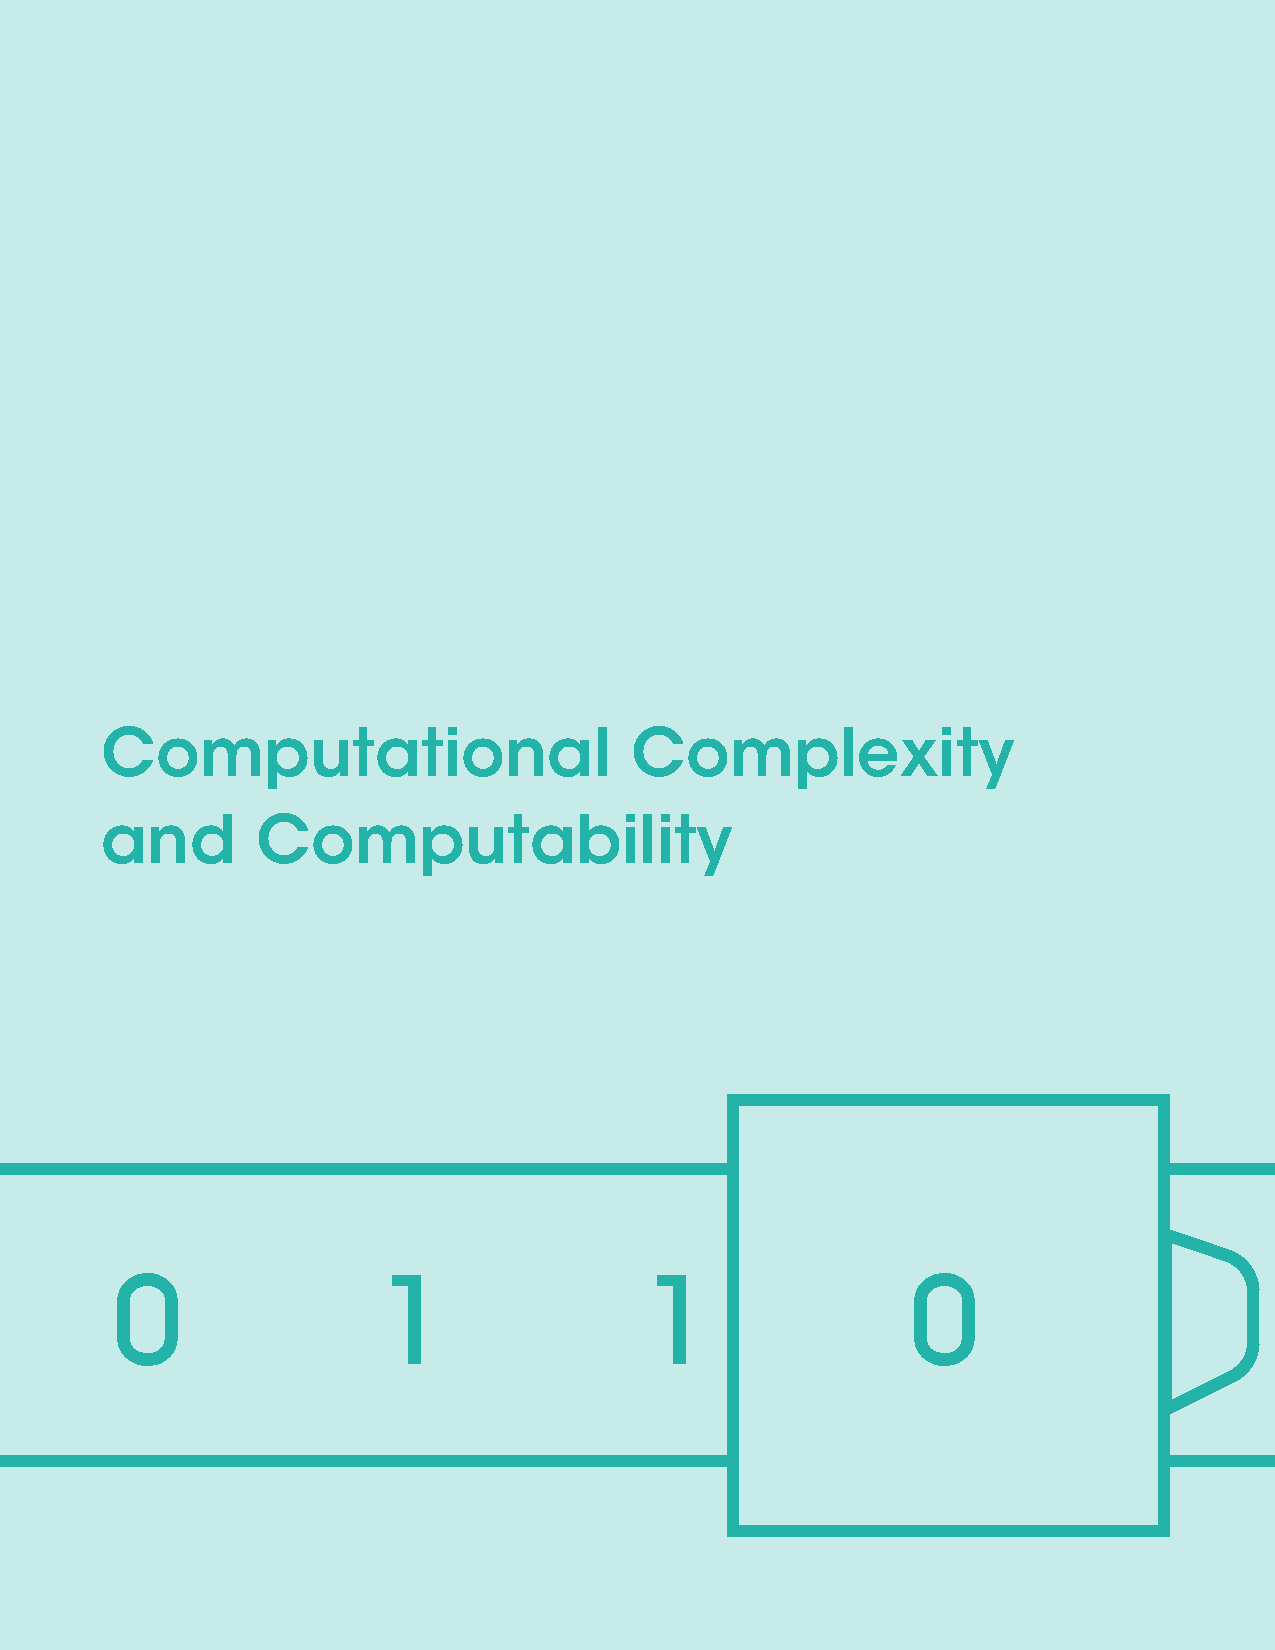
\includepdf[pages=-]{complexity_cover.pdf}

%----------------------------------------------------------------------------------------
%	COPYRIGHT PAGE
%----------------------------------------------------------------------------------------

\newpage
The cover depicts a Turing machine. Turing machine is a simple but powerful computation model used to study the computability and complexity of problems. It is considered one of the foundational models of theoretical computer science.
~\vfill
\thispagestyle{empty}

\noindent Copyright \copyright\ \the\year{} Kevin Gao % Copyright notice

\hfill

\noindent \textsc{terra-incognita.dev} % URL

\hfill

% License information
\noindent Licensed under the Creative Commons Attribution-NonCommercial 3.0 Unported License (the ``License''). You may not use this file except in compliance with the License. You may obtain a copy of the License at \url{http://creativecommons.org/licenses/by-nc/3.0}. Unless required by applicable law or agreed to in writing, software distributed under the License is distributed on an \textsc{``as is'' basis, without warranties or conditions of any kind}, either express or implied. See the License for the specific language governing permissions and limitations under the License.


%----------------------------------------------------------------------------------------
%	TABLE OF CONTENTS
%----------------------------------------------------------------------------------------

%\usechapterimagefalse % If you don't want to include a chapter image, use this to toggle images off - it can be enabled later with \usechapterimagetrue

 % Table of contents heading image

\pagestyle{empty} % Disable headers and footers for the following pages
\usechapterimagefalse
\tableofcontents % Print the table of contents itself

\cleardoublepage % Forces the first chapter to start on an odd page so it's on the right side of the book

\pagestyle{fancy} % Enable headers and footers again

%----------------------------------------------------------------------------------------
%	PART
%----------------------------------------------------------------------------------------
\setlength{\parskip}{1em}

\part{Automata and Languages}

\chapter{Regular Language}
\section{Alphabet and Strings}

$\Sigma$ denotes a finite alphabet of symbols. $\Sigma^*$ denotes a set of all strings, including the empty string $\epsilon$, consist of elements of $\Sigma$.

For string $x \in \Sigma^*$, $|x|$ is the length of $x$. A language is a subset of $\Sigma^*$.

\section{Regular Language}

See 240 notes.

Example: $\\mathrm{Even} = \{ w \in \{0,1\}^* \mid \text{$w$ contains an even number of 1's}\}$. It can be expressed using the regular expression $0^* + (0^*10^*10^*)^*$.

It also has a 2-state deterministic finite automaton that decides the language $\mathsf{Even}$.
\begin{center}
    \begin{tikzpicture}
    \node[state,initial,accepting] (qeven) {\( q_{even} \)};
    \node[state] (qodd) [right=of qeven] {\( q_{odd} \)};
    \path[->] (qeven) edge [above,bend left=20] node {1} (qodd);
    \path[->] (qodd) edge [below,bend left=20] node {1} (qeven);
    \path[->] (qeven) edge [loop above] node {0} (qeven);
    \path[->] (qodd) edge [loop above] node {0} (qodd);
    \end{tikzpicture}
\end{center}

More formally,
\begin{definition}[Deterministic Finite State Automata]
    A deterministic finite state automaton (DFA) is a quintuple (5-tuple)
    $$
    M = (Q,\Sigma,\delta,s,F)
    $$
    where
    \begin{itemize}
        \item $Q$ is a finite set of states
        \item $\Sigma$ is a finite set called the alphabet
        \item $\delta:\, Q\times\Sigma \to Q$, the transition function
        \item $s \in Q$, the starting state
        \item $F \subseteq Q$, the set of accepting states
    \end{itemize}
\end{definition}

\chapter{Context-Free Language}
\input{notes/cfl.tex}

\chapter{Turing Machine}
\section{Turing Machine}

While finite state automata and pushdown automata are all valid models of computation, they are too restricted as models of general purpose computers. Our goal is to have a model so that we can define computation as abstractly and general as possible.

How do we define algorithms rigorously? What does it mean for an algorithm to run in polynomial time. How do we argue that efficient algorithms do not exist.

Turing machine is a model of computation first proposed by Alan Turing in 1936. It is much more powerful than previous models that we have looked at. It is sufficiently general and can model what a human can do. A Turing machine can be think of a finite automata with unlimited and unrestricted memory.

In a Turing machine, we have an \textbf{one-way infinite tape} divided into ``cells'', each holding one symbol, including the blank symbol $\sqcup$. It also has a \textbf{read-write} head positioned in one square at a time that can move to the left or right. The control of the Turing is in of a fixed number of states. (The blank symbol $\sqcup$ is sometimes denoted by $\not b$ or $\square$ )

Initially, the input tape contains a finite number of symbols starting at the left-most cell with the remaining cells blank. The head starts at the left-most input symbol. Current state and symbol determine the next state, symbol written, and the movement of the head (either one square left or one square right).

\begin{figure}[htbp]
    \centering
    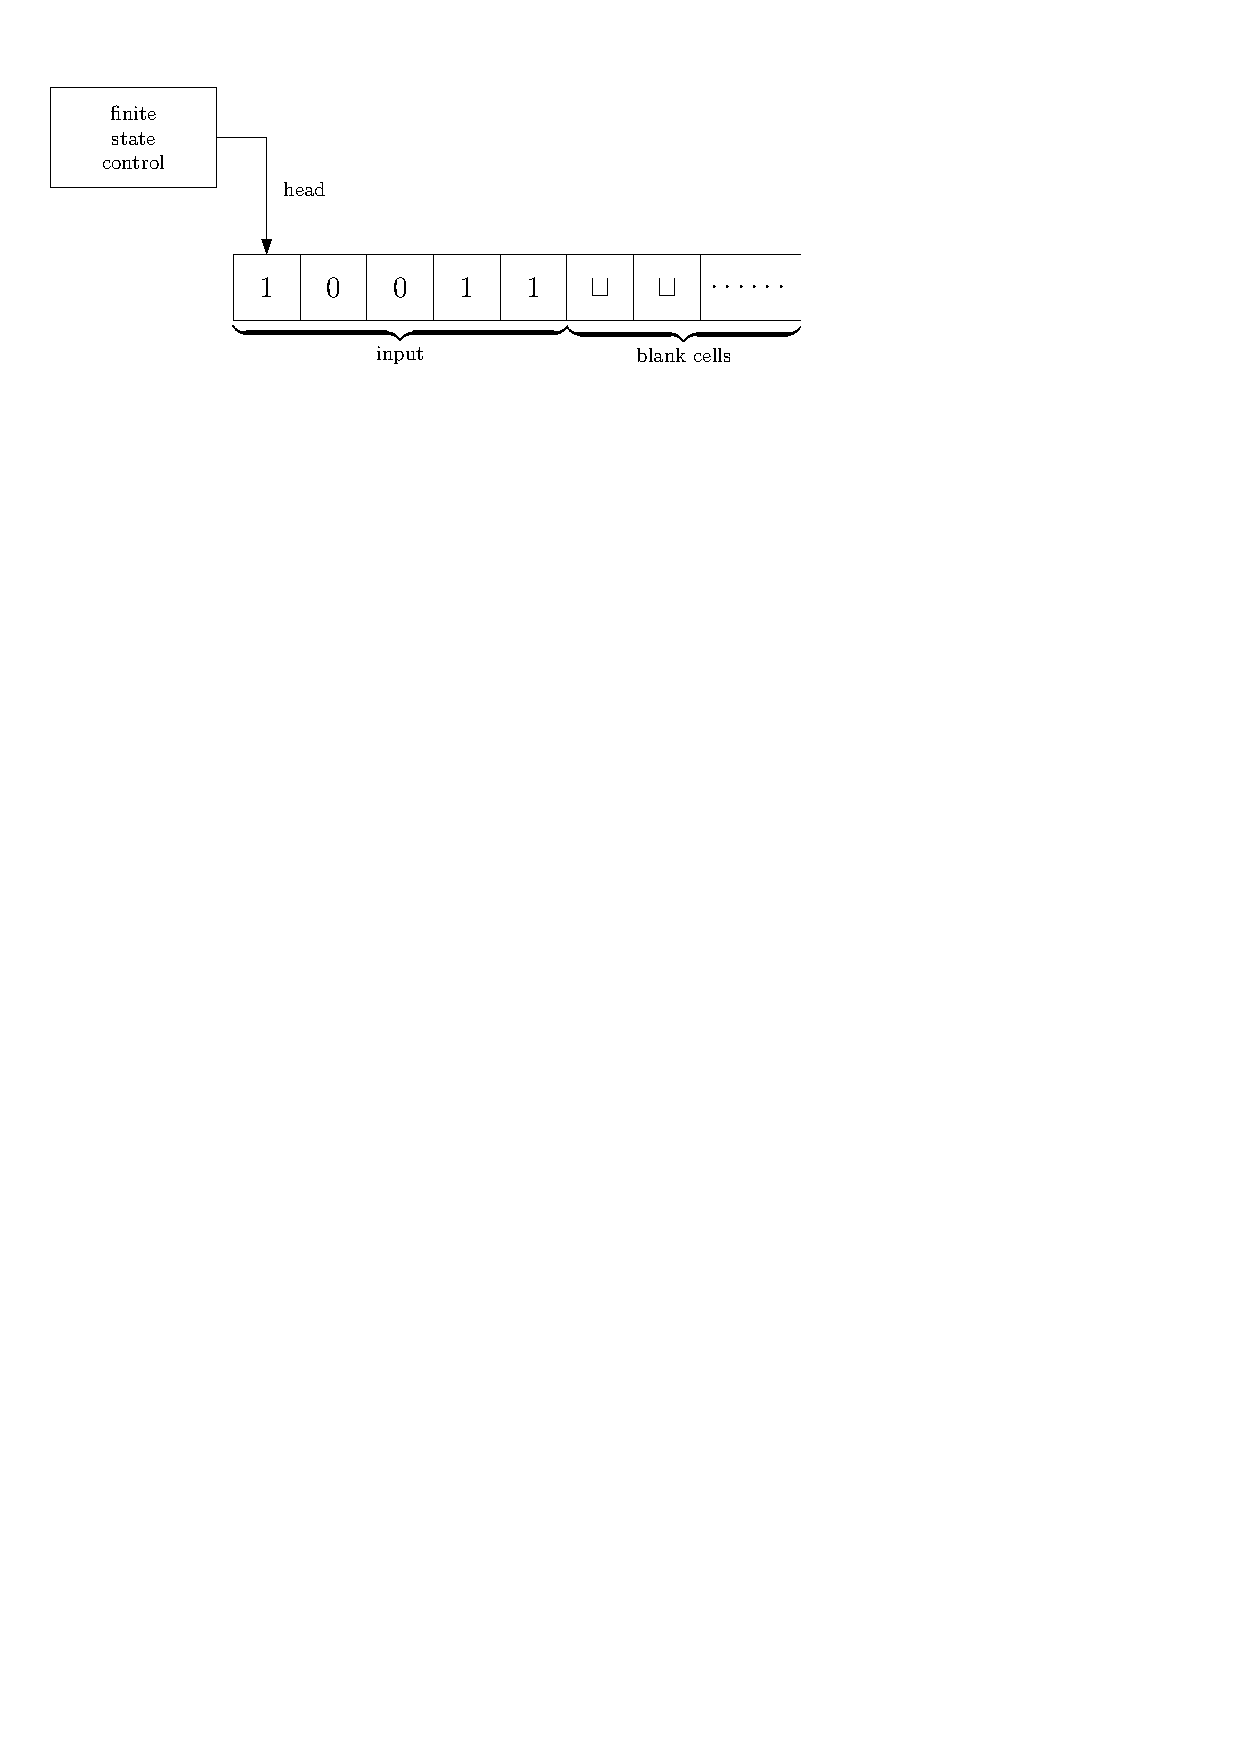
\includegraphics[width=0.7\linewidth]{tm.pdf}
    \caption{A Turing machine}
    \label{fig:tm}
\end{figure}

\begin{definition}[Turing Machine]
    A Turing machine is a 7-tuple $(Q,\Sigma,\Gamma,\delta,q_0,q_{accept},q_{reject})$ where $Q,\Sigma,\Gamma$ are all finite sets, and
    \begin{itemize}
        \item $Q$ is the set of states
        \item $\Sigma$ is the input alphabet not containing the blank symbol $\sqcup$
        \item $\Gamma$ is the tape alphabet, where $\sqcup \in \Gamma$ and $\Sigma \subset \Gamma$
        \item $\delta:\;(Q-\{q_{accept},q_{reject}\}) \times \Gamma \to Q \times \Gamma \times \{L,R\}$ is the transition function
        \item $q_0 \in Q$ is the start state
        \item $q_{accept} \in Q$ is the accept state
        \item $q_{reject} \in Q$ is the reject state, where $q_{accept} \neq q_{reject}$ 
    \end{itemize}
\end{definition}

$\delta(q,a) = (q',a',x)$ where $x \in \{L,R\}$ means if a machine is in state $q$ and head positioned on a square containing $a$, then the machine replaces $a$ with $a'$, moves to state $q$, and moves the head left ($L$) or right ($R$) depending on the direction given by $x$.

A Turing machine $M$ works as follows on input string $x \in \Sigma^*$.
\begin{enumerate}
    \item Initially $x = x_1x_2\ldots x_n \in \Sigma^*$ appears on leftmost $n$ squares of the input tape. Rest of the tape is blank;
    \item Head of $M$ starts on the leftmost square of tape;
    \item Initial state is $q_0$ 
    \item $M$ moves according to the transition function $\delta$
    \item Continue until $M$ reaches $q_{accept}$ or $q_{reject}$ and then $M$ halts. Otherwise, continue on forever.
\end{enumerate}

\begin{definition}[Language Recognized by Turing Machine]
    We say a Turing machine $M$ \textbf{accepts} a string $x \in \Sigma^*$ if $M$ upon reading the input $x$ eventually \textbf{halts} in state $q_{accept}$.

    Let $L(M) = \{x \in \Sigma^* \mid \text{$M$ accepts $x$} \}$. We say $L(M)$ is the \textbf{language recognized/accepted by} $M$. We say $x \not\in L(M)$ if $M$ upon reading $x$ either \textbf{halts} in $q_{reject}$ or \textbf{loops}.
\end{definition}

\begin{example}[Palindrome]
    $$\mathrm{Palindrome} = \{yy^R \mid y \in \{0,1\}^*\}$$
    At a high level, the \textbf{Turing machine} that decides this language scans back and forth, matching and erasing leftmost and rightmost symbols. Accept if the input is completely earased or reject if otherwise.
\end{example}

\section{Configuration of Turing Machine}

The \textbf{configuration} of a Turing machine describes the state, head position, and tape contents. It is denoted $x q y$ where $x,y \in \Gamma^*$ and $q \in  Q$. In this notation, the head position is implied to be the leftmost symbol of $y$.

Note that $xqy$ and $xqy \sqcup$ are equivalent configurations, but $xqy$ and $\sqcup xqy$ are not equivalent. Whether or not the first symbol is blank is important.

\begin{definition}
    Given two configurations $C_1$ and $C_2$, we say configuration $C_1$ \textbf{yields} $C_2$ if $C_2$ follows from $C_1$ by one step of $M$ (one application of $\delta$).
\end{definition}

\begin{example}
    Let $x,y \in \Gamma^*$ and $a,b \in \Gamma$. If $\delta(q,a) = (q',a',R)$, then $xqay$ yields $xa'q'y$. If $\delta(q,b) = (q',b',L)$, then $xaqby$ yields $xq'ab'y$. $qby$ yields $q'b'y$ because the tape head cannot move left anymore.
\end{example}

\begin{definition}[Computation]
    The \textbf{computation} of $M$ on input $x \in \Sigma^*$ is the sequence $C_0C_1C_2\ldots$ where $C_0 = q_0x$ and each configuration follows from the previous one. We say the computation is \textbf{halting} if it eventually reaches accept or reject state. Otherwise, we say the computation is \textbf{looping} (infinite).
\end{definition}

\section{Decidability and Recognizability}

\begin{definition}[Decider]
    A Turing machine $M$ is a decider if it halts on all inputs $x \in \Sigma^*$.
\end{definition}

\begin{definition}[Turing Decidable and Turing Recognizable]
    A language $A \in \Sigma^*$ is Turing decidable if and only if there is a \textbf{decider} $M$ such that $L(M)=A$.

    $A$ is semidecidable/Turing recognizable if and only if there is a Turing machine $M$ such that $L(M)=A$. In this case, $M$ may not halt if it does not accept $A$ (reject by looping).
\end{definition}

\section{Some Classes of Languages}

$\textsf{D} = \{ A \subseteq \Sigma^* \mid \text{$A$ is decidable}$

$\textsf{SD} = \{A \subseteq \Sigma^* \mid \text{$A$ is semidecidable}$

$\textsf{P} = \{A \subseteq \Sigma^* \mid \text{$A=L(M)$ for some $M$ that halts in polynomial time} \}$

Later, we will show that $\textsf{P} \subsetneq \textsf{D} \subsetneq \textsf{SD}$.

\section{Difference Between FSA and TM}

\begin{itemize}
    \item TM can read and write symbols. Infinite tape.
    \item Head can move left or right, unless the head is at left-most position.
    \item Special ``accept'' and ``reject'' states that stop computation immediately. The machine halts only when it reaches an accept or reject state. On the other hand, an FSA can only perform a finite amount of transitions before it halts.
\end{itemize}

\part{Decidability and Computability}

\chapter{Undecidable Language}
\section{Countability}

\vspace{\parskip}

\begin{definition}[Countable Set]
    A set $A$ is countable if $A$ is empty or there is a injective function $f:\, A \to \N$, or equivalently, a surjective function $f:\, \N \to A$.
\end{definition}

\begin{theorem}
    $\R$ is not countable.
\end{theorem}

\begin{theorem}
    $2^{\N} = \mathcal{P}(\N)$ is not countable.
\end{theorem}

\begin{corollary}
    There exists some $A \subseteq \Sigma^*$ such that $A$ is not Turing-recognizable.
\end{corollary}

\begin{proof}
    We will prove this by showing that the set of all languages in $\Sigma^*$ is not countable, but the set of Turing-recognizable languages is countable.

    We first show that $\Sigma^*$ is countable. To show this, we simply list all strings in $\Sigma^*$ in lexicographic order.

    Observe that $\mathsf{TR} = \{ A \subseteq \Sigma^* \mid A = L(M) \}$ is also countable because the number of Turing machines is countable, each of which can be encoded as a finite length string.

    But the set of all languages $\{ A \subseteq \Sigma^* \} = 2^{\Sigma^*}$. By Cantor's theorem, since $\Sigma^*$ is countably infinite, the power set of $\Sigma^*$ is uncountable.

    Hence, there exists some language $A \subseteq \Sigma^*$ that is not Turing-recognizable.
\end{proof}

Let $\langle M \rangle$ denote the encoding of a Turing machine $M$. For $n \in \N$, let $\langle n \rangle \in \{0,1\}^*$ be the binary encoding of $n$. For a sequence of numbers $n_1,n_2,\ldots,n_k$, $\langle n_1,n_2,\ldots,n_k \rangle \in \{0,1,\#\}^*$ be $\langle n_1 \rangle \# \langle n_2 \rangle \# \cdots \# \langle n_k \rangle$.

Then, any Turing machine can be determined by a finite sequence of numbers specifying $|Q|$, $|\Sigma|$, $|\Gamma|$, identity of $q_0,q_{accept},q_{reject}$, and a sequence of numbers specifying $\delta$.

$$
\langle M \rangle = \text{the string that determines $M$}
$$

Furthermore, we can denote a Turing machine $T$ with input $w$ as $\langle M, w \rangle$.

\begin{theorem}
    Let
    $$
    \mathsf{DIAG} = \{ \langle M \rangle \mid \text{$M$ is a TM and $\langle M \rangle \not\in L(M)$} \}
    $$
    $\mathsf{DIAG}$ is not Turing recognizable.
\end{theorem}

\begin{proof}
    Suppose, for contradiction, that there exists a TM $M$ such that $T(M) = \mathsf{DIAG}$. Then, we can ask if $\langle M \rangle \in L(M)$.

    Suppose that $\langle M \rangle \in L(M)$. Then
    $$
    \langle M \rangle \in L(M) \iff \langle M \rangle \in \mathsf{DIAG} \iff \langle M \rangle \not\in \in L(M)
    $$
    which is a contradiction.
\end{proof}

This is similar to Russell's paradox.

\begin{theorem}
    Every finite language is Turing recognizable and decidable.
\end{theorem}

\begin{theorem}
    Every regular language is Turing recognizable and decidable.
\end{theorem}

\section{Universal Turing Machine}

Let $A_{\mathsf{TM}}$ be the language
$$
\{ \langle M,w \rangle \mid \text{$M$ accepts $w$} \}
$$

\begin{theorem}
    $A_{\mathsf{TM}}$ is Turing-recognizable.
\end{theorem}

\begin{proof}
    We show that there exists a TM $U$ such that $L(U) = A_{\mathsf{TM}}$. $U$ decodes $\langle M \rangle$ into a TM $M$ and simulates $M$ on $w$. Thus, $A_{\mathsf{TM}}$ is Turing-recognizable.
\end{proof}

The $U$ that we have constructed to recognize $A_{\mathsf{TM}}$ is called a universal Turing machine.

\begin{theorem}
    $A_{\mathsf{TM}}$ is not decidable.
\end{theorem}

\chapter{Reducibility}
\section{Proving Undecidability by Reduction}

\begin{theorem}
    $A_{\mathsf{TF}}$ is not decidable.
\end{theorem}

\begin{proof}
    By contradiction.

    Suppose that $A_{\mathsf{TM}}$ is decidable. Then there exists some Turing machine that decides $A_{\mathsf{TM}}$. We will derive a contradiction by showing that if $A_{\mathsf{TM}}$ is decidable, then $\mathsf{DIAG}$ must also be decidable.

    To decide $\encoding{M} \in \mathsf{DIAG}$, we feed $\encoding{ M,\encoding{M} }$ into a Turing machine that decides $A_{\mathsf{TM}}$. 
\end{proof}

\begin{corollary}
    Let $\mathsf{D}$ be the class of decidable languages, and let $\mathsf{TR}$ is the class of Turing-recognizable.
    $$
    \mathsf{D} \subsetneq \mathsf{TR}
    $$
\end{corollary}

Let $\overline{A} = \{ w \in \Sigma^* \mid w \not\in A \} = \Sigma^* - A$.

Let $\coTR = \{ A \mid \overline{A} \in \mathsf{TR} \}$.

\begin{theorem}
    If $A \subseteq \Sigma^*$, then $A \in \mathsf{D} \iff A \in \TR\, \land\, \overline{A} \in \TR$.
\end{theorem}

\begin{proof}
    Suppose $A \in \TR \cap \coTR$. Let $M_1$ be a TM that recognizes $A$. Let $M_2$ be a TM that recognizes $\overline{A}$.

    Let $M$ be a multi-tape Turing machine that simulates $M_1$ and $M_2$ in parallel. On input $w$, since $w \in A$ or $w \not\in A$, either $M_1(w)$ accepts or $M_2(w)$ accepts. If $M_1$ accepts, then $M$ accepts. If $M_2$ accepts, then $M$ rejects.
\end{proof}

\section{Closure Properties}

\subsection{Union, Intersection, and Complement}

\begin{theorem}[Closure Under Union, Intersection, and Complement]
    If $A,B \in \D$, then $A \cup B \in \D$, $A \cap B \in \D$, and $\overline{A} \in \D$.
\end{theorem}

\begin{theorem}
    The class of languages $\TR$ is closed under union, intersection, but NOT under complement.
\end{theorem}

An intuitive explanation for why $\TR$ is not closed under complement, then this would imply that all languages in $\TR$ would also be decidable.

\begin{proof}
    Consider $A_{\TM} \in \TR$. If $\overline{A_{\TM}} \in \TR$, then $A_{\TM} \in \coTR$, which implies that $A_{\TM} \in \D$. A contradiction.  
\end{proof}

\begin{proof}
    Let $A,B \in \TR$. Then $A = L(M_1)$ and $B = L(M_2)$ for some TM $M_1$ and $M_2$.

    $A \cap B = L(M_{A\cap B})$ where $M_{AB}$ on input $w$ runs $M_1$ and $M_2$ in parallel on two tapes and accepts if and only if $M_1$ and $M_2$ both halts and accepts.

    $A \cup B = L(M_{A \cup B})$ where $M_{AB}$ on input $w$ runs $M_1$ and $M_2$ in parallel on two tapes and accepts if either $M_1$ or $M_2$ halts and accepts.
\end{proof}

\section{Computable Functions}

So far, we have been using TM to accept and reject inputs. However, we can also use a TM to compute a function. If a function can be computed (evaluated) using a Turing machine, we say the function is computable.

\begin{definition}[Computable Function]
    A function $f:\, \Sigma^* \to \Sigma^*$ is computable if there is some Turing machine $M$ on every input $w \in \Sigma^*$, $M$ halts with $f(w)$ on the tape.
\end{definition}

\begin{example}[Duplicate]
    Consider the function
    $f(w) = w \cdot w$ 
    that duplicates a string $w$.
\end{example}

Note that $f$ can take as input $\encoding(M)$ and output an encoding for some other Turing machine $\encoding{M'}$.

\begin{example}[Example of Uncomputable Function - Halting Problem]
    The function
    $$
    h(\encoding{\encoding{M},w}) = \begin{cases}
        1 & \text{if $M$ halts on input $w$} \\
        0 & \text{if $M$ does not halt on input $w$}
    \end{cases}
    $$
    solves the Halting problem and hence is not computable.
\end{example}

\begin{theorem}[Church-Turing Thesis]
    Any function that can be computed by an ``algorithm'', then the function is computable.
\end{theorem}

It can be shown by the diagonal argument that the set of all functions is uncountable, and hence not all functions are computable because the set of computable functions is countable.

\section{Mapping Reducible}

\begin{definition}[Mapping Reducible]
    A language $A$  is mapping reducible to $B$, denoted $A \leq_m B$ if there is a computable function $f:\; \Sigma^* \to \Sigma^*$ where for every $w$,
    $$
    w \in A \iff f(w) \in B
    $$
\end{definition}

\begin{figure}[htbp]
    \centering
    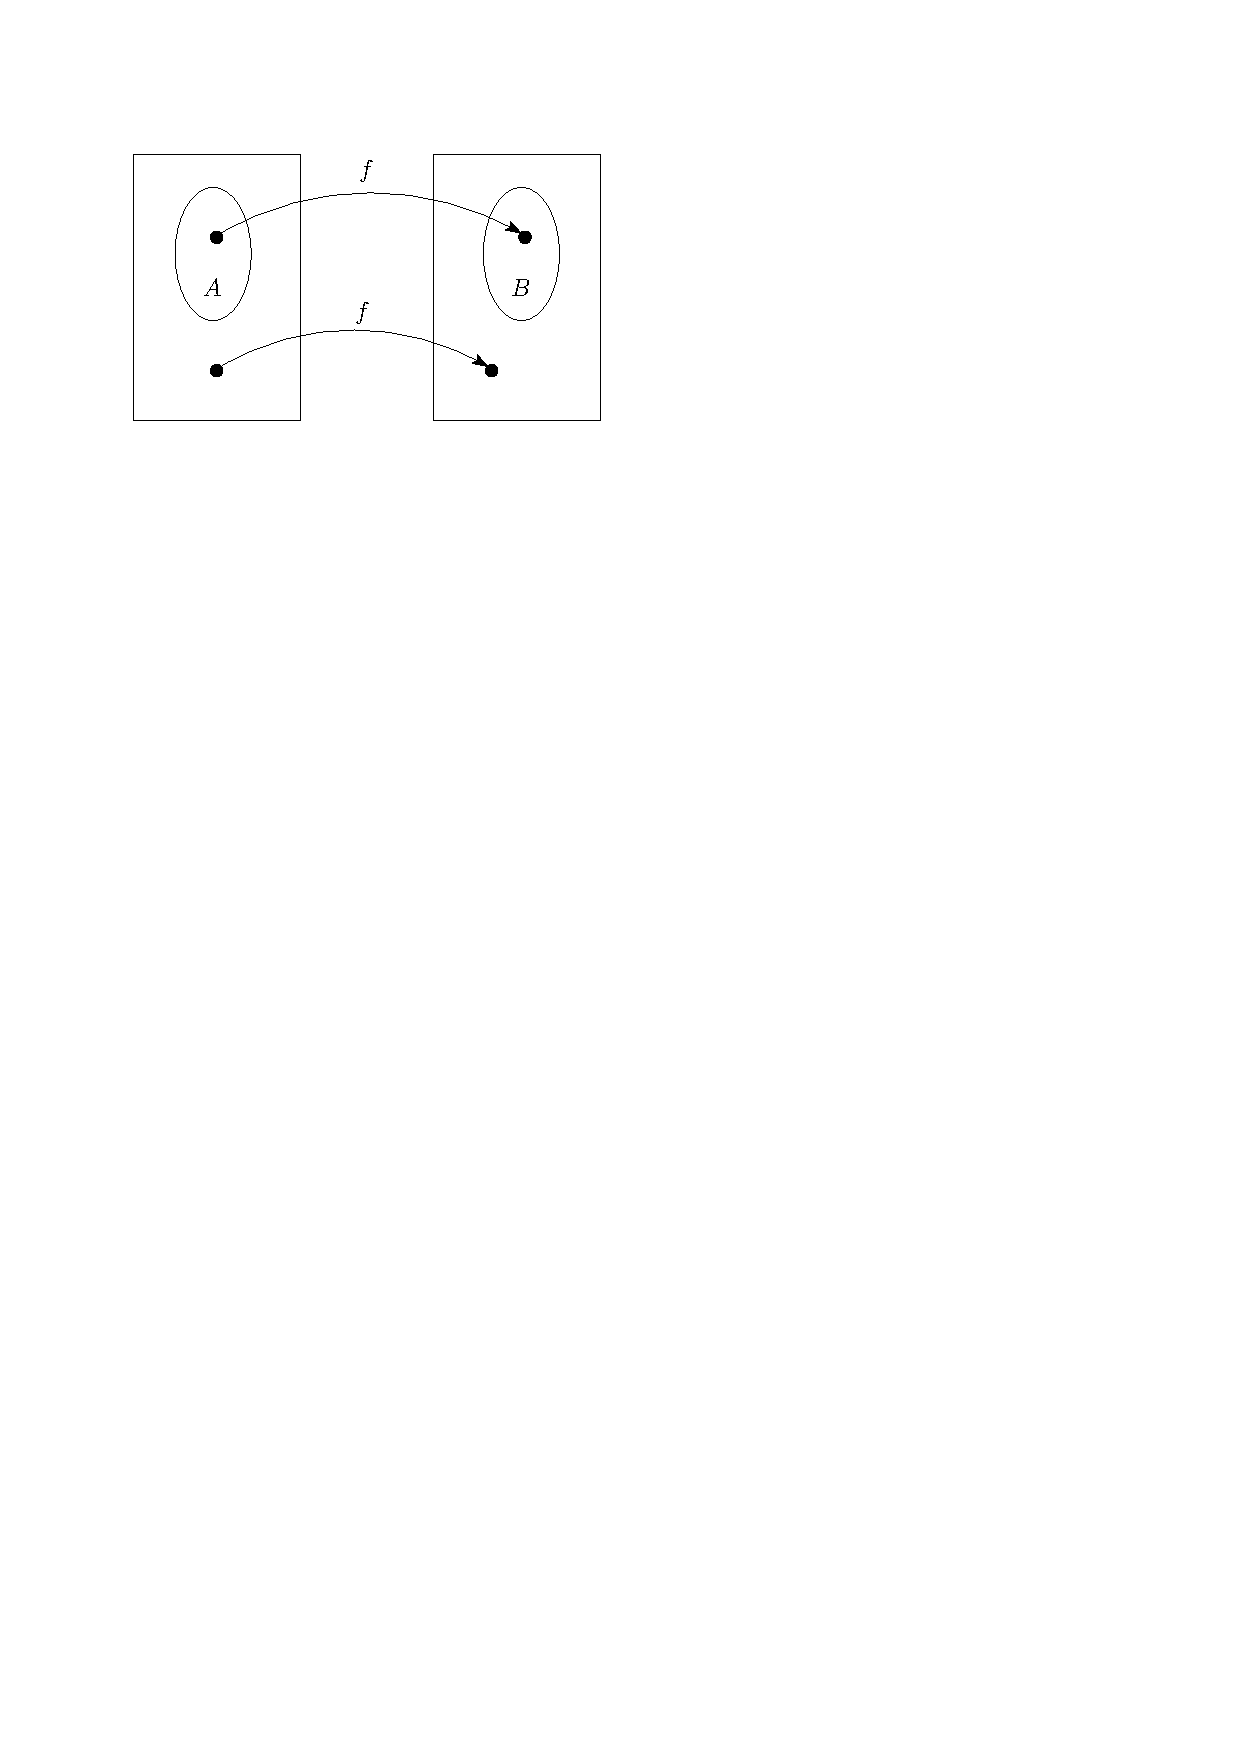
\includegraphics[width=0.4\linewidth]{mapping-reduction.pdf}
    \caption{Function $f$ reducing $A$ to $B$.}
    \label{fig:mapping-reduction}
\end{figure}

Observation: If $A \leq_m B$, then $\overline{A} \leq_m \overline{B}$. If $A \leq_m B$ and $B \leq_m C$, then $A \leq_m C$ (this follows from function composition).

\begin{remark}
    Later, we will see other types of reductions. For example, $\leq_p$ for polytime reduction.
\end{remark}

\begin{theorem}
    If $A \leq_m B$ and $B$ is decidable, then $A$ is decidable. If $B$ is Turing-recognizable, then $A$ is also Turing-recognizable.
\end{theorem}

\begin{proof}
    Let $M$ be a decider for $B$. Let $f$ be the computable mapping reduction from $A$ to $B$, and let $N$ be the Turing machine that computes this function.

    Then $A$ is decided by a Turing machine which on input $w$, runs $N$ to obtain $f(w)$ and then runs $M$ on $f(w)$.
\end{proof}

\begin{corollary}
    If $A \leq_m B$ and $A$ is not decidable, then $B$ is not decidable.
\end{corollary}

Application: Consider $\Diag = \{ \encoding{M} \mid \encoding{M} \not\in \lang(M) \}$. Then, $\Diag \leq_m \overline{A_{\TM}}$ via the reduction $f:\, \Sigma^* \to \Sigma^*$ defined as
$$
f(\encoding{M}) = \encoding{M,\encoding{M}}
$$
and if the input $w$ to $f$ is not an encoding of a TM, then
$$
f(w) = \encoding{M_{accept}, \epsilon}
$$

Since $\Diag$ is not decidable, $\overline{A_{\TM}}$ is not decidable.

\section{Applications of Reduction}

\subsection{Halting Problem}

Consider the language
$$
\Halt_{\TM} = \{ \encoding{M,w} \mid \text{$M$ halts on $w$} \}
$$

We have $\Halt_{\TM} \leq_m A_{\TM}$ and $A_{\TM} \leq_m \Halt_{\TM}$.

\begin{proof}

    \hfill
    
    ($\Halt_{\TM} \leq_m A_{\TM}$): If $x$ is any string of the form $\encoding{M,w}$, then $f(x) = \encoding{M',w}$ where $M'$ accepts if and only if $M$ halts on input $w$. $M'$ will simulate $M$ running on $w$ and accepts when $M$ halts. If $x$ is not of the correct form, $f(x) = \encoding{M_{loop},\epsilon}$.

    ($A_{\TM} \leq_m \Halt_{\TM}$): If $x$ is a string of the form $\encoding{M,w}$, then $f(x) = \encoding{M',w}$ where $M'$ simulates $M$ on $w$, and halts if and only if $M$ accepts. If $x$ is not of the correct form, then $f(x) = \encoding{M_{loop}, \epsilon}$.
\end{proof}

\begin{corollary}
    $\Halt_{\TM}$ is mapping equivalent (equivalent under mapping reduction) to $A_{\TM}$.
    $$
    \Halt_{\TM} \equiv_{m} A_{\TM}
    $$
\end{corollary}

Hence,
$$
\begin{aligned}
    \Halt_{\TM} &\in \TR \\
    &\not\in \coTR \\
    &\not\in \D
\end{aligned}
$$

\subsection{EQ}

Consider the language
$$
\EQ_{\TM} = \{ \encoding{M_1,M_2} \mid \text{$M_1$ and $M_2$ are Turing machines and $\lang(M_1) = \lang(M_2)$} \}
$$

We show that
$$
A_{\TM} \leq_{m} \EQ \qquad \text{and} \qquad A_{\TM} \leq_m \overline{\EQ}
$$

\begin{proof}
    Given $\encoding{M,w}$, if $M$ accepts $w$, we want to output $M_1,M_2$ such that $\lang(M_1) = \lang(M_2)$.

    Let $M_1$ be the TM which accepts all inputs. $\lang(M_1) = \Sigma^*$.
    
    Let $M_2$ be the TM which on any input, runs $M$ on $w$ and accepts if and only if $M$ accepts.

    So, $f(\encoding{M,w}) = \encoding{M_1,M_2}$.

    $$
    \lang(M_2) = \begin{cases}
        \Sigma^* & \text{if $M$ accepts $w$} \\
        \emptyset & \text{otherwise}
    \end{cases}
    $$

    Reduction from $A_{\TM}$ to $\overline{\EQ}$.
\end{proof}

Let $A$ be a set of TM descriptions $\{\encoding{M_1},\encoding{M_2},\ldots\}$. Show that if $A \in \TR$, then there is some set of TM descriptions $B \in \D$ such that the set of associated languages of $A$ and $B$ are the same. Formally,
$$
\{ \lang(M) \mid \encoding{M} \in A \} = \{ \lang(M) \mid \encoding{M} \in B \} 
$$
Let $E_B$ be an enumerator for $B$.
\begin{codebox}
    \li $\id{prev-length} = 0$
    \li \For $\encoding{M_1},\encoding{M_2},\ldots$ from $E_A$ \Do
        \li $M' = \proc{Pad}(\encoding{M_1},\, \id{prev-length} + 1)$
        \li $\id{prev-length} = |\encoding{M'}|$
        \li \textbf{print} $\encoding{M'}$
\end{codebox}
$\lang(E_B)$ is the decidable language that is the same as the language recognized by Turing machines in $A$.

Let $A \in \TR$ be a recognizable set of decider descriptions. Show that there is some decidable set $B$ such that $B$ is not the language of any TM in $A$.

Let $A = \{\encoding{D_1},\encoding{D_2},\ldots\}$. We want to show that there exists some $B$ such that $\forall i.\, B \not \in \lang(D_1)$. Let $\encoding{D_1},\encoding{D_2},\ldots$ be an enumeration of $A$. Also, let $w_1,w_2,\ldots$ be an enumeration of $\Sigma^*$ in standard string order.

Let $B = \{ w_i \mid w_i \not\in \lang(D_i) \}$. We first show that $B$ is decidable. We can construct a decider for $B$ as follows.
\begin{codebox}
    \Procname{$D_B(x)$}
    \li determine $i$ such that $w_i = x$
    \li run the enumerator for $A$ to get $\encoding{D_i}$ 
    \li simulate $D_i$ on $w_i = x$ 
    \li \If $D_i$ accepts \Then
        \li \textbf{reject}
    \li \Else
        \li \textbf{accept}
\end{codebox}

We then show that $B \not\in \lang(D_i)$ for some $\encoding{D_i} \in A$. If $w_i \in B$, then $w_i \not\in \lang(D_i)$, and $B \neq\lang(D_i)$. If $w_i \not\in B$, then $w_i \in \lang(D_i)$ and $B \neq \lang(D_i)$.

A language $A$ is recognizable if and only if there is a decider $V$ such that for all $x \in \Sigma^*$,
$$
x \in A \iff \exists y.\, \text{$V$ accepts $(x,y)$}
$$
Think $V$ as a verifier and $y$ as a ``certificate'' that $x \in A$.

$L$ is recognizable by TM $M$.
\begin{codebox}
    \Procname{$V(x,y)$}
    \li simulate $M$ on $x$ for $|y|$ steps
    \li \If $M$ accepts \Then
        \li \textbf{accept}
    \li \ElseIf $M$ rejects or has not completed \Then
        \li \textbf{reject}
    \End
\end{codebox}
If $x \in A$, then $M$ accepts within a finite number of steps $k$. Then, $V(x,\, y=1^k)$.

Now suppose that there exists a decider $V$ such that for all $x \in A$, there exists $y \in \Sigma^*$ such that $V$ accepts $(x,y)$.

We need to find a recognizer for $A$.

\begin{codebox}
    \Procname{$M(x)$}
    \li \For $y \in \Sigma^*$ \Do
        \li run $V(x,y)$ 
        \li \If $V$ accepts \Then
            \li \textbf{accept}
        \li \Else
            \li \textbf{continue}
\end{codebox}

If $x \in A$, there exists $y$ such that $V(x,y)$ accepts, then $y$ eventually show up in the standard string order of $\Sigma^*$ and when $y$ is run on $V$, $V$ accepts. Otherwise, $M$ loops.

\section{Rice's Theorem}

Using reduction, we can prove a really strong theorem about the decidability of certain languages, which can cover many of the languages that we have discussed so far.

\begin{theorem}[Rice's Theorem]
    Suppose $P$ is a language of Turing machine descriptions such that
    \begin{enumerate}
        \item $P$ is nontrivial: it contains some but not all Turing machine descriptions;
        \item $P$ is a \textit{\textbf{property of the Turing machine's languages}} (instead of a property of the Turing machine itself): whenever $\lang(M_1) = \lang(M_2)$, then $\encoding{M_1} \in P \iff \encoding{M_2} \in P$.  
    \end{enumerate}
    Then, $P$ is decidable.
\end{theorem}

Here are some example languages that are covered by Rice's theorem.
\begin{example}
    \hfill
    \begin{itemize}
        \item $\mathrm{EMPTY}_{\TM} = \{ \encoding{M} \mid \lang(M) = \emptyset \}$
        \item $\mathrm{FINITE}_{\TM} = \{ \encoding{M} \mid \text{$\lang(M)$ is finite} \}$
        \item $\mathrm{DECIDABLE}_{\TM} = \{ \encoding{M} \mid \text{$\lang(M)$ is decidable} \}$
    \end{itemize}
    Rice's theorem claims that all of these languages are undecidable.

    Note that Rice's theorem does not apply to $\{ \encoding{M} \mid \text{$M$ is a decider} \}$ because the property being satisfied by the TM descriptions in this language is a property of the Turing machine itself, not its language. Criterion 2 of Rice's theorem is not satisfied.
\end{example}

Now, let's prove Rice's theorem using reduction.

\begin{proof}
    Let $T_0$ be the TM which always rejects. Without loss of generality, suppose that $\encoding{T_0} \not\in P$. Otherwise, we can consider $\overline{P}$ which also satisfies the criteria for Rice's theorem.
    
    Since $P$ is nontrivial, there exists TM $T_1$ such that $\encoding{T_1} \in P$. We will show that $\ATM \leq_m P$. In this end, we map $\encoding{M,w}$ to $M_w$ where
    $$
    \begin{aligned}
        M_w = ``
        &\text{on input $x$} \\
        &\text{1. Simulate $M$ on $w$} \\
        &\text{2. If $M$ rejects $w$, reject} \\
        &\begin{aligned}
            \text{3. } &\text{If $M$ accepts $w$, then run $T_1$ on $x$} \\
            &\text{$M_w$ accepts/rejects/loops according to what $T_1$ does on input $x$}"
        \end{aligned}
    \end{aligned}
    $$
    $\lang(M_w)$ is either $\emptyset = \lang(T_0)$ or the langauge of $T_1$, $\lang(T_1)$, depending on whether $w$ is accepted by $M$.

    \textit{Claim}. $\encoding{M,w} \in \ATM \iff \encoding{M_w} \in P$.

    If $M$ accepts $w$, then $\lang(M_w) = \lang(T_1)$, so $M_w \in P$. \\
    If $M$ rejects $w$, then $\lang(M_w) = \emptyset = \lang(T_0)$, so $\encoding{M_w} \not\in P$. \\
    If $M$ loops on $w$, $M_w$ loops on all inputs so $\lang(M_w) = \emptyset = \lang(T_0)$.
\end{proof}

\chapter{Computation History Method}
\section{Configuration and Computation History}

Recall that the \textit{\textbf{configuration}} of a Turing machine can be expressed as a triple $(q,p,t)$ where $q$ is the current state, $p$ is the head position, and $t$ is the tape content. Equivalently, this can be written as an encoding $t_1qt_2$ where $t = t_1t_2$ and the head position is on the first symbol of $t_2$.

\begin{example}[Configuration of a Turing Machine]
    For example, the configuration 
    $$(q_3,6,aaaaaabbbbb)$$
    means the Turing machine is in state $q_3$, with the head pointing at the 6th symbol, and the current tape content being $aaaaaabbbbb$. This can be expressed in a more compact form as
    $$
    aaaaa q_3 abbbbb
    $$
\end{example}

A computation history of a Turing machine is a sequence of configurations of the Turing machine until it reaches an accepting state.

\begin{definition}[Computation History]
    An \textit{\textbf{accepting computation history}}, or \textit{\textbf{computation history}}, for a Turing machine $M$ on input $w$ is a sequence of configurations $C_1,C_2,\ldots,C_{accept}$ that $M$ enters until it accepts. Each configuration in this sequence is yielded from the configuration immediately before it.
    
    We encode a computation history as a sequence of configurations separated by the pound sign \#.
    $$
    C_1 \# C_2 \# \ldots \# C_{accept}
    $$
\end{definition}

\begin{example}
    A computation history for $M$ on $w = w_1w_2\ldots w_n$ given $\delta(q_0,w_1) = \delta(q_7,a,R)$ and $\delta(q_7,w_2) = (q_8,c,R)$ is as follows
    $$
    \underbrace{q_0w_1w_1 \ldots w_n}_{C_1} \# \underbrace{aq_7w_2 \ldots w_n}_{C_2} \# \underbrace{acq_8w_3 \ldots w_n}_{C_3} \# \cdots \# \underbrace{\ldots q_{accept} \ldots}_{C_{accept}}
    $$
\end{example}

\section{Decidability of Problems Concerning Linearly Bounded Automata}

To understand how to prove undecidability using the computation history method, we first examine a type of machine known as linearly bounded automata (LBA).

\begin{definition}[Linearly Bounded Automaton]
    A \textit{\textbf{linearly bounded automaton (LBA)}} is a single-tape Turing machine that cannot move its head off the input portion of the tape. In other words, the size of the tape is restricted to the size of the input.
\end{definition}

\subsection{A\textsubscript{LBA} is Decidable}

Let
$$
\A_{\LBA} = \{ \encoding{B,w} \mid \text{LBA $B$ accepts $w$} \}
$$
Although it may come as surprising at a first glance, $\A_{\LBA}$ is, in fact, decidable. This is because of the fac that, for an LBA of input size $n$, the number of configurations of the LBA is finite, namely equal to $|Q| \times n \times |\Gamma|^n$.

\textit{Claim}. For inputs of length $n$, an LBA can only have $|Q| \times n \times |\Gamma|^n$ configurations.

\begin{theorem}
    $\A_{\LBA}$ is decidable.
\end{theorem}

\begin{proof}
    If $B$ on $w$ runs for too long (more than $|Q| \times n \times |\Gamma|^n$), then by the pigeonhole principle, $B$ must be looping and will never halts or accept. More formally, let us construct a decider for $\A_{\LBA}$.
    $$
    \begin{aligned}
        D_{\A_{\LBA}} = 
            `` &\text{on input $\encoding{B,w}$} \\
            &\text{1. Let $n = |w|$} \\
            &\text{2. Run $B$ on $w$ for $|Q| \times n \times |\Gamma|^n$ steps} \\
            &\text{3. If $B$ has accepted, accept} \\
            &\text{4. If $B$ has rejected or it is still running, reject}
            ''
    \end{aligned}
    $$
\end{proof}

\subsection{E\textsubscript{LBA} is Undecidable}
Now, let us consider the language
$$
\E_{\LBA} = \{ \encoding{B} \mid \text{$B$ is an LBA and $\lang(B) = \emptyset$} \}
$$
The next natural question is whether or not $\E_{\LBA}$ is also decidable. We will show using reduction that $\ATM$ can be reduced to $\E_{\LBA}$ and thus $\E_{\LBA}$ is undecidable.

\begin{theorem}
    $\E_{\LBA}$ is undecidable.
\end{theorem}

\begin{proof}
    Assume that $\E_{\LBA}$ is decidable. Then, there exists a Turing machine $R$ that decides $\E_{\LBA}$. We construct a Turing machine $S$ deciding $\ATM$.
    $$
    \begin{aligned}
        S = 
            `` &\text{on input $\encoding{M,w}$} \\
            &
            \begin{aligned}
                \text{1. } &\text{Construct LBA $B_{\encoding{M,w}}$ that tests whether its input $x$ is an accepting computation history} \\
                &\text{for $M$ on $w$, and accepts only if $x$ is an accepting computation history}
            \end{aligned} \\
            &\text{2. Use $R$ to determine whether $\lang(B_{\encoding{M,w}}) = \emptyset$} \\
            &\text{3. Accept if no. Reject if yes.}
            ''
    \end{aligned}
    $$
    More specifically, we define $B_{\encoding{M,w}}$ as follows.
    $$
    \begin{aligned}
        B_{\encoding{M,w}} = 
        `` &\text{on input $x$} \\
        &\text{1. Check if $x$ begins $C_1 \#$ where $C_1$ is the start configuration of $M$ on $w$} \\
        &\text{2. Check if each $C_{i+1}$ yields from $C_i$ } \\
        &\text{3. Check if the final configuration is accepting} \\
        &\text{4. Accept if all checks pass. Otherwise, reject.}
    \end{aligned}
    $$
    Clearly, $S$ accepts if and only if $M$ on $w$ accepts, and it halts on all inputs. Hence, $S$ decides $\ATM$, but since $\ATM$ is undecidable, this is a contradiction.
\end{proof}

\section{Post Correspondence Problem}

A domino has the form $\displaystyle \left[ \frac{t}{b} \right] $ where $t, b \in \Sigma^*$.

Given a collection of dominos $\displaystyle P = \left\{ \left[ \frac{t_1}{b_1} \right], \ldots, \left[ \frac{t_k}{b_k} \right] \right\}$, we say there is a \textit{\textbf{match}} if we can make a list using the dominos from $P$ (possibly with repetitions) such that the whole string on the top row is equal to the whole string on the bottom row. The \textit{\textbf{Post Correspondence Problem (PCP)}} is to determine whether a collection of dominos $P$ has a match. That is, we want to determine if there is a sequence $i_1,i_2,\ldots,i_m \in \{1,2,\ldots,k\}$ such that $t_{i_1} \cdot t_{i_2} \cdot \ldots \cdot t_{i_m} = b_{i_1} \cdot b_{i_2} \cdot \ldots \cdot b_{i_m}$.

Figure \ref{fig:pcp-example} shows a set of dominos and a match.

\begin{figure}[htbp]
    \centering
    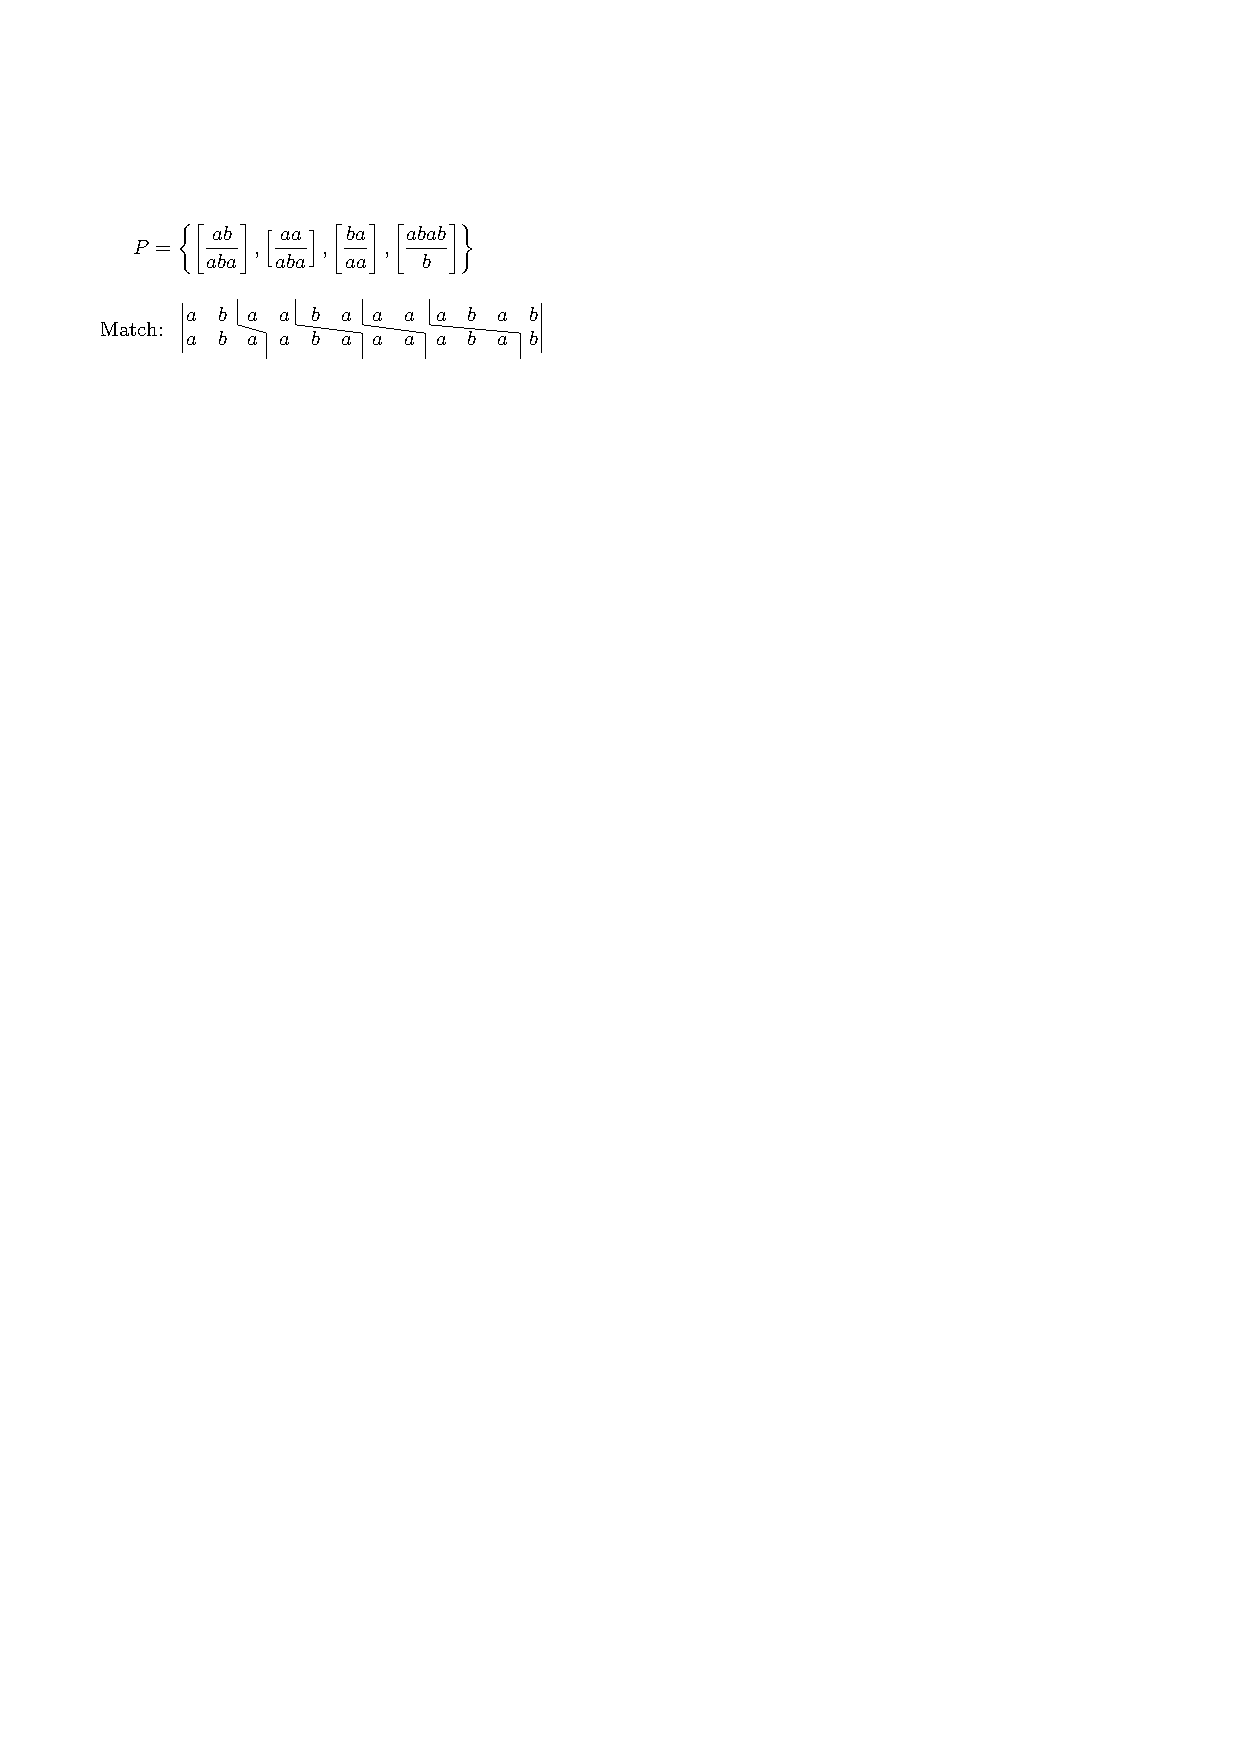
\includegraphics[width=0.6\linewidth]{pcp-example.pdf}
    \caption{A set of dominos $P$ and the corresponding match.}
    \label{fig:pcp-example}
\end{figure}

\begin{theorem}
    $\PCP$ is undecidable.
\end{theorem}

The main idea of the proof: reduction $\ATM \leq_m \PCP$ using computation histories. We will in fact show two reductions:
$$
\ATM \leq_m \MPCP \leq_m \PCP
$$

To make the proof simpler, we first restrict ourselves to the Modified Post Correspondence Problem (MPCP). MPCP adds the additional requirement that the match starts with the first domino $\left[ \frac{t_1}{b_1} \right]$.

\begin{proof}[Proof \hspace{0.1em} ($\ATM \leq_m \MPCP$)]
    Let $M = (Q,\Sigma,\Gamma,\delta,q_0,q_{acc},q_{rej})$ such that $w \in \Sigma^*$.

    We are given $\encoding{M,w}$ as input and must construct a set of dominos $P$ such that $P$ has a match if and only if $M$ accepts on input $w$. We assume, without loss of generality, $M$ never attempts to move head left when its head is in the leftmost position.

    Given $\encoding{M,w}$, we construct $P$. To do that, we introduce the following types of dominos. We put each type of dominos in the order as they are introduced below.

    \textbf{Step 1}: $\displaystyle \left[ \frac{\#}{\# q_0 w_1 w_2 \ldots w_n \#} \right]$ or $\displaystyle \left[ \frac{\#}{\# q_0 \sqcup} \right]$ if $w = \epsilon$.

    This domino is used as the first domino, which simulates the initial configuration of $M$.

    \textbf{Step 2}: For all $a,a' \in \Gamma$ and $q,q' \in Q$ where $q \neq q_{rej}$, if $\delta(q,a) = (q',a',R)$, we put the domino
    $$
    \left[ \frac{qa}{a'q'} \right] 
    $$
    This domino simulates the transitions where the head moves to the right.

    \textbf{ 3}: For all $a,a',b \in \Gamma$ and $q,q' \in Q$ where $q \neq q_{rej}$, if $\delta(q,a) = (q',a',L)$, we put the domino
    $$
    \left[ \frac{bqa}{q'ba'} \right] 
    $$
    This domino simulates the left movement of the head.

    \textbf{Step 4}: For every $a \in \Gamma$, we put $\displaystyle \left[ \frac{a}{a}\right]$.
    
    This domino fills in the remaining contents of the tape after a transition.

    \textbf{Step 5}: $\displaystyle \left[ \frac{\#}{\#} \right]$ and $\displaystyle \left[ \frac{\#}{\sqcup\#} \right]$
    
    This domino places the delimiter marking the end of a configuration.

    We repeat Step 2-5 to simulate the configurations of $M$ until it reaches the accepting configuration. After all these are finished, we should have a sequence of dominos of the form

    \begin{center}
        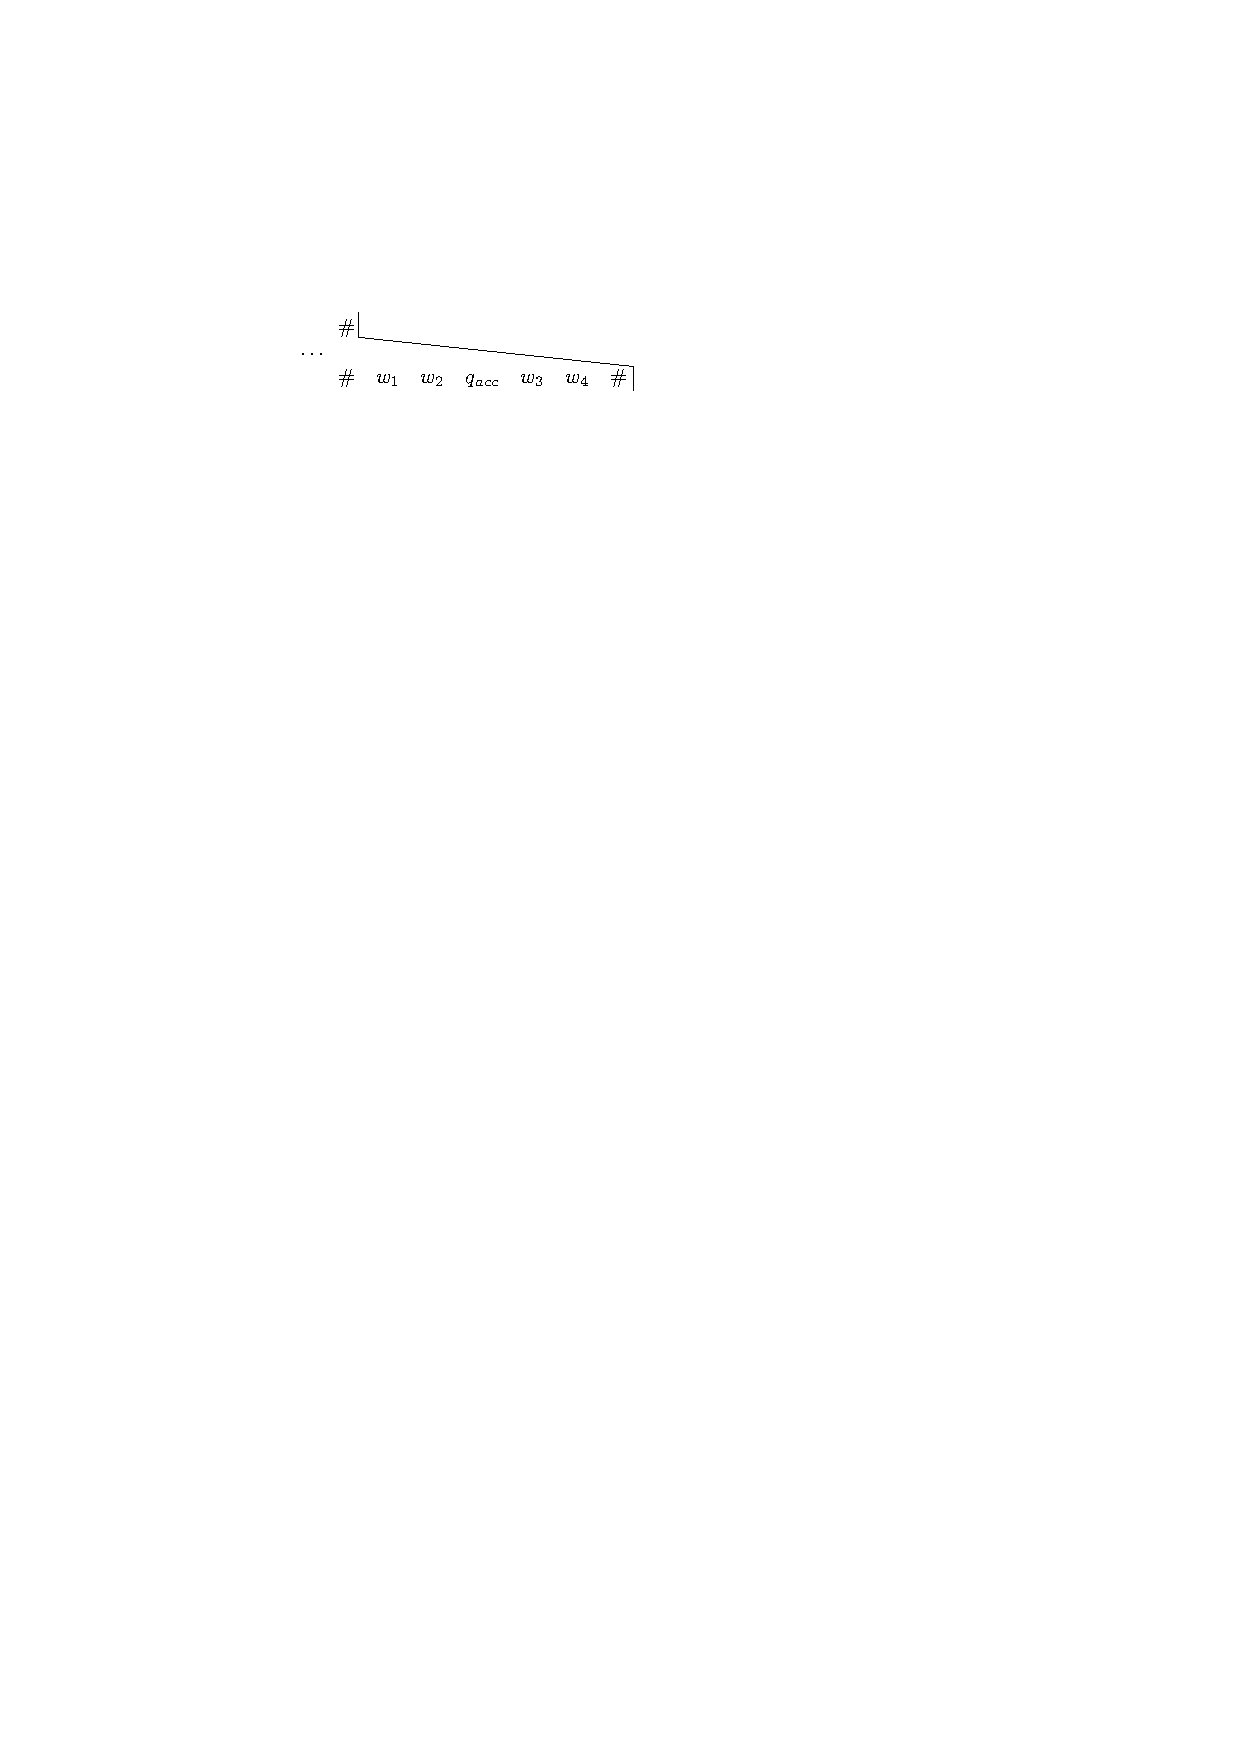
\includegraphics[width=0.4\linewidth]{pcp-step5.pdf}
    \end{center}

    \textbf{Step 6}: For every $a \in \Gamma$, put
    $$
    \left[ \frac{a q_{acc}}{q_{acc}} \right]  \quad \text{and} \quad \left[ \frac{q_{acc} a}{q_{acc}} \right]
    $$
    This step eats away the symbols adjacent to $q_{acc}$ at the bottom, one at a time, as illustrated below.
    \begin{center}
        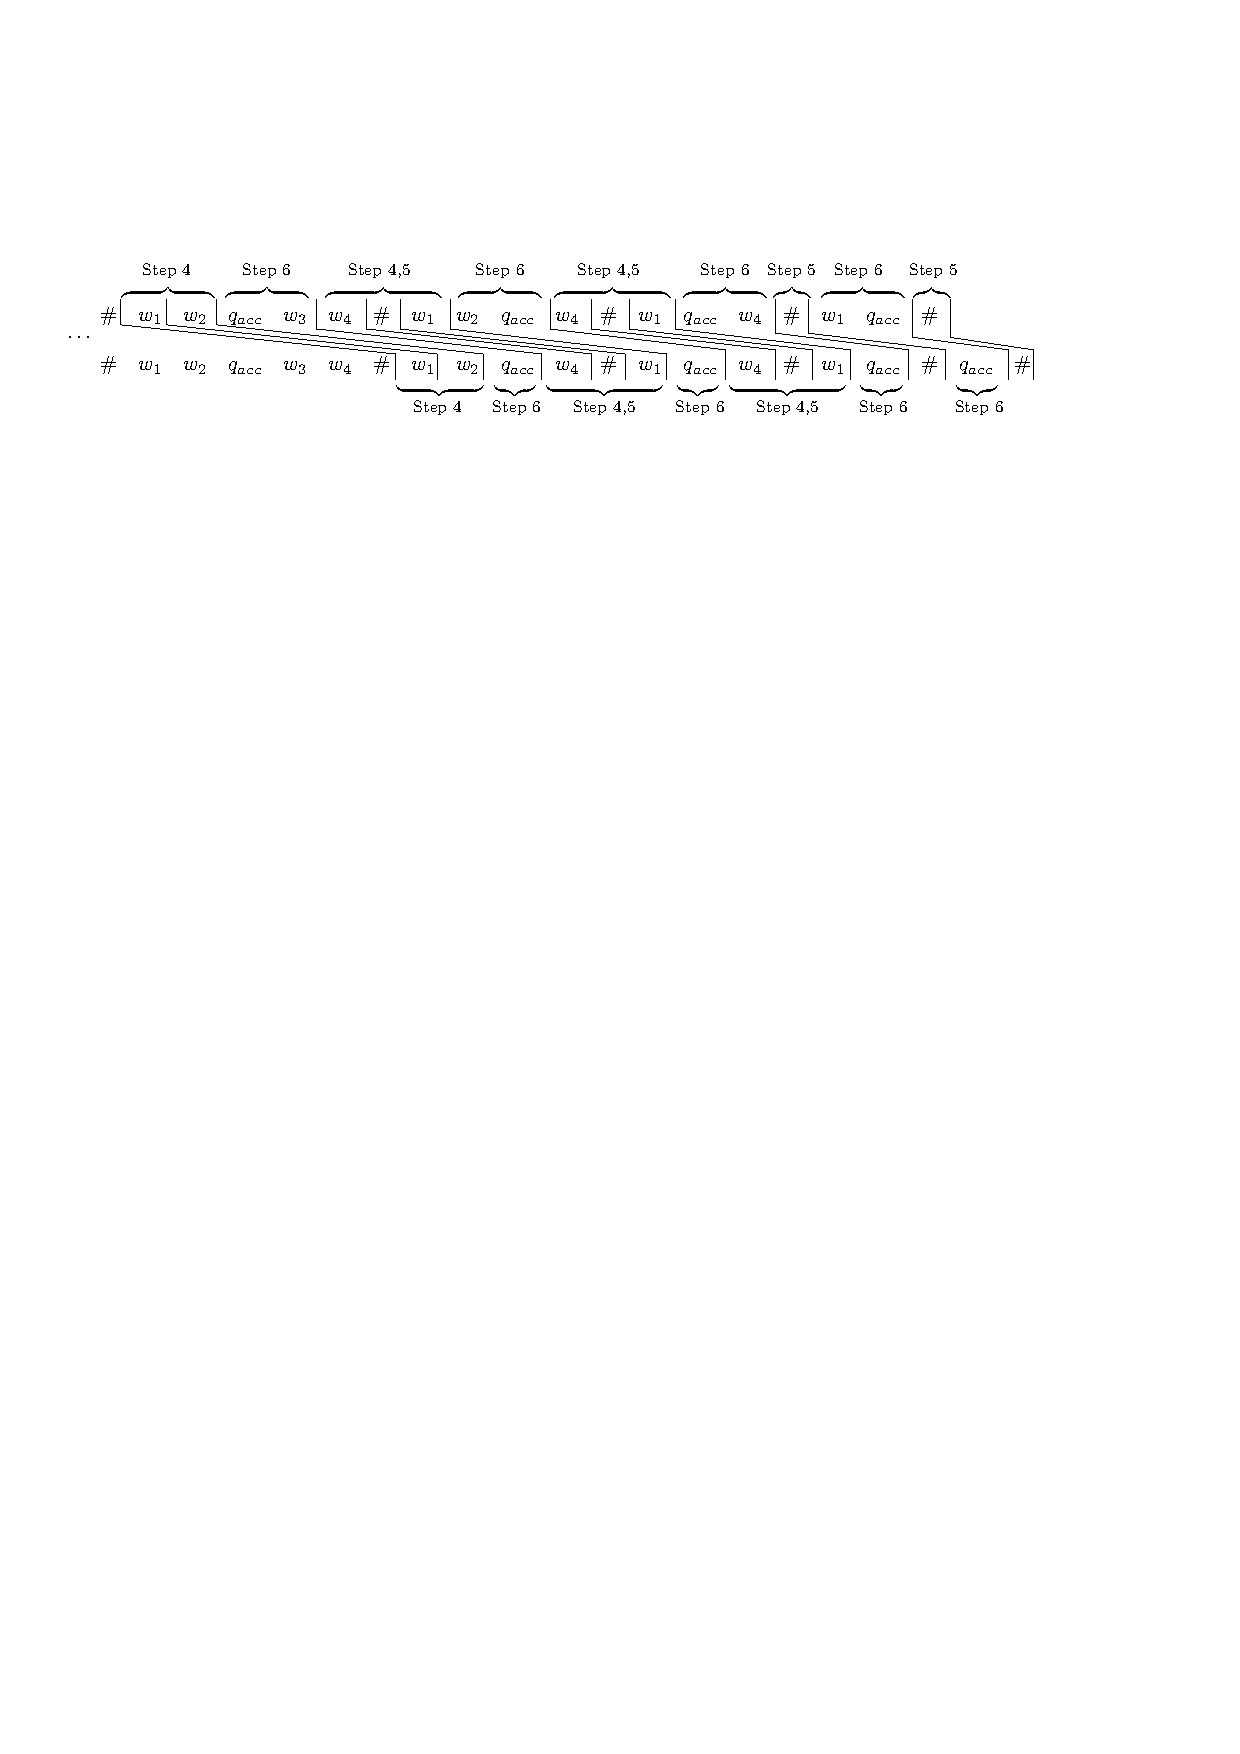
\includegraphics[width=0.9\linewidth]{pcp-step6.pdf}
    \end{center}

    Finally, \\
    \textbf{Step 7}: Put the domino $\displaystyle \left[ \frac{q_{acc} \#\#}{\#} \right]$. This step finishes off the alignment of the top and bottom row.
    \begin{center}
        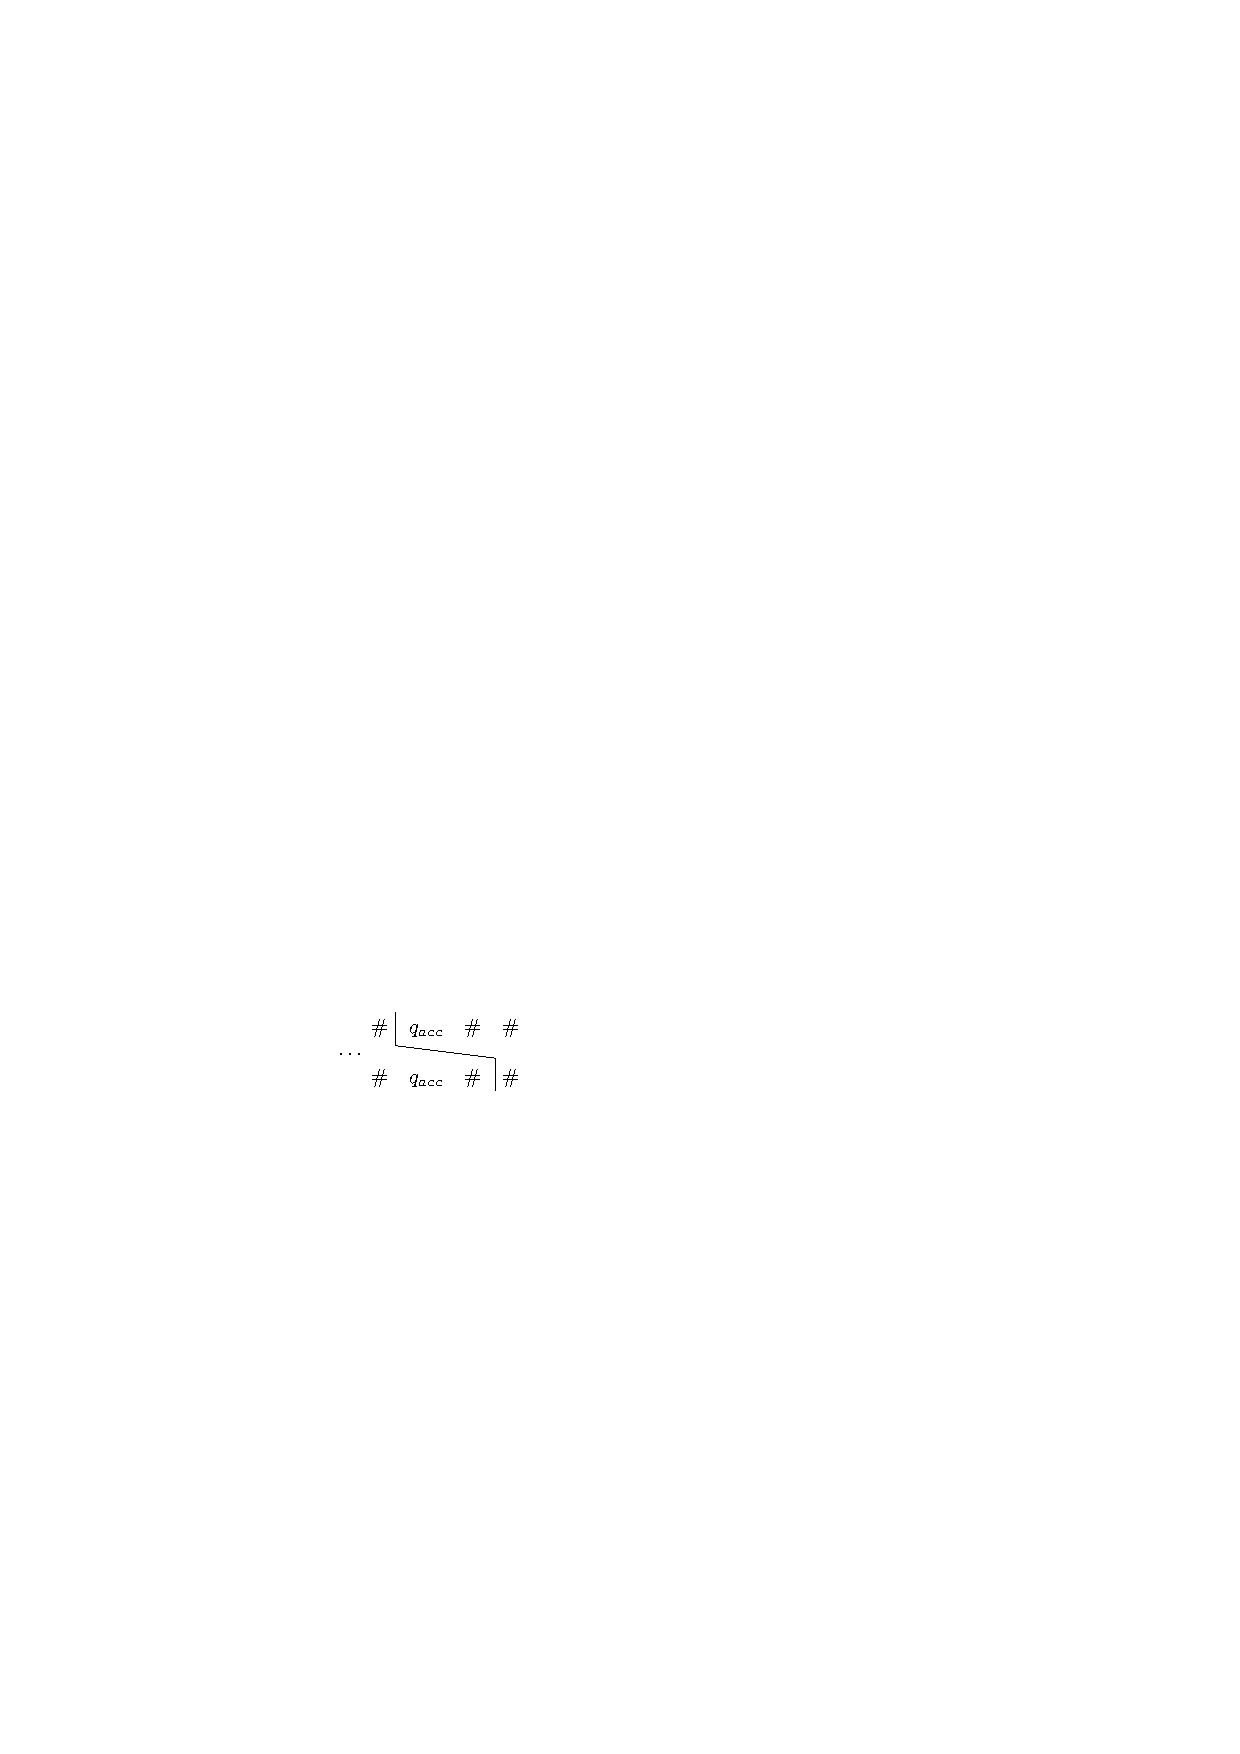
\includegraphics[width=0.2\linewidth]{pcp-step7.pdf}
    \end{center}

    This concludes the construction of $P$.

    \textit{Claim}. $P$ is an accepting instance of MPCP $\iff$ $M$ accepts $w$. 

    \hfill

    Next, we provide the construction that shows $\MPCP \leq_m \PCP$. It trivially holds that any accepting instance of MPCP is also a PCP. To see why, consider the match $\left[ \frac{\#}{\#} \right]$.

    Now, we show how to convert an instance of MPCP to PCP such that the converted instance still simulates $M$ on $w$. Let $\displaystyle P = \left\{ \left[ \frac{t_1}{b_1} \right], \ldots, \left[ \frac{t_k}{b_k} \right] \right\}$ be an input to MPCP. Further, let $\{*, \diamond\}$ be new symbols that are not in any $t_i$ or $b_i$.

    For any string $u = u_1u_2\ldots u_n$, let
    $$
    \begin{aligned}
        \circledast u &= * u_1 * u_2 \ldots * u_n \\
        u \circledast &= u_1 * u_2 * \ldots u_n * \\
        \circledast u \circledast &= * u_1 * u_2 * \ldots * u_n *
    \end{aligned}
    $$
    Consider the domino set $P'$ 
    $$
    P' = \left\{ \left[ \frac{\circledast t_1}{\circledast b_1 \circledast} \right]  \right\} \cup \left\{ \left[ \frac{\circledast t_i}{ b_i \circledast} \right]  \mid 1 \leq i \leq k \right\} \cup \left\{ \left[ \frac{* \diamond}{\diamond} \right]  \right\}
    $$
    Then, there is a match in $P$ starting with $\left[ \frac{t_1}{b_1} \right] $ if and only if there is a match in $P'$. The only domino in $P'$ that could start a match is $\left[ \frac{\circledast t_1}{\circledast b_1 \circledast} \right]$ because it is the only one where both the top string and bottom string starts with *.
\end{proof}

\chapter{Information}
\section{Quantifying Information}

Can we quantify how much information is in a string.

Consider
$$
x = 0101010101010101
$$
and
$$
y = 110001010110010
$$
Intuitively, $y$ appears to have more information than $x$, which is simply repeated $01$.

We would like to have a formal definition that captures the intuitive definition of ``information''.

Idea: The more we can compress a string, the less information it contains.

Thesis: The amount of information in a string is the shortest way to describe the string.

Consider $\encoding{M,w}$, where $M(w)$ halts with only $x$ on its tape. We need to specify an encoding of $\encoding{M,w}$ (what is the alphabet, and when does $\encoding{M}$ end and $w$ begin).

There are different encodings. For the purpose of our discussion, we restrict outselves to binary strings. A specific encoding of $\encoding{M,w}$, let $M$ be a TM with input alphabet $\{0,1\}$ and $w = w_1w_2\ldots w_n \in \{0,1\}^*$.

If $\encoding{M} = z_1z_2\ldots z_k \in \{0,1\}^*$ is a binary encoding of $M$, let
$$
\encoding{M,w} = 0 z_1 0 z_2 \ldots 0 z_k 1 w_1 w_2 \ldots w_n
$$ 
Then, $|\encoding{M,w}| = 2 |\encoding{M}| + |w| + 1$. We use 0 to separate each character in the Turing machine description, and we use 1 to separate $\encoding{M}$ and $w$.

Alternatively, we can use 11 to represent 1 in the description of $\encoding{M}$, 00 to represent 0; additionally, use 01 as the delimiter separating $\encoding{M}$ and $w$. This is the encoding presented in Sipser.

\begin{definition}[Shortest Description]
    If $x \in \{0,1\}^*$, then the \textit{\textbf{shortest description}} $x$, denoted $d(x)$ is the lexicographically minimal string $\encoding{M,w}$ such that $M(w)$ halts with only $x$ on its tape.
\end{definition}

\begin{definition}[Kolmogorov Complexity]
    The \textit{\textbf{Kolmogorov complexity}} (or descriptive complexity, Kolmogorov-Chaitin complexity) of $x$, denoted $K(x)$ is $|d(x)|$.
\end{definition}

\begin{theorem}
    There is a constant $c$ such that for all $x \in \{0,1\}^*$,
    $$
    K(x) \leq |x| + c
    $$
\end{theorem}
The amount of information in $x$ is not much more than $|x|$. The Kolmogorov complexity of a string is at most a fixed constant more than its length.

\begin{proof}
    Define $M$
    
    $M$ on input $w$, halts. On any string $x$, $M(x)$ halts with $x$ on its tape.
    $$
    K(x) \leq |\encoding{M,x}| \leq 2|\encoding{M}| + |x| + 1 \leq |x| + c
    $$ 
    So we can let $c$ be the length of the trivial Turing machine that computes the identity function.
\end{proof}

\begin{theorem}
    There exists a constant $c$ such that for all $x \in \{0,1\}^*$,
    $$
    K(xx) \leq K(x) + c
    $$
\end{theorem}

This says if a string is repetitive, such string has no more information than $x$.

\begin{proof}
    Consider the Turing machine $M$ defined as follows
    $$
    \begin{aligned}
        M = ``&\text{on input $\encoding{N,w}$, where $N$ is a TM and $w$ is a string} \\
        &\text{1. Run $N$ on $w$ until it halts and produces an output string $s$} \\
        &\text{2. Output the string $ss$ }"
    \end{aligned}
    $$
    Let $\encoding{M,w}$ be the shortest description of $x$, then $\encoding{N,\encoding{M,w}}$ is a description of $xx$.
    $$
    K(xx) \leq |\encoding{N,\encoding{M,w}}| \leq 2|\encoding{N}| + K(x) + 1 \leq K(x) + c
    $$
    So letting $c = 2|\encoding{N}| + 1$, the theorem holds.
\end{proof}

\begin{corollary}
    There is a constant $s$ such that for all $n\geq 2$ and $x \in \{0,1\}^*$,
    $$
    K(x^n) \leq K(x) + c \log n
    $$
    In particular, $K((01)^n) \in O(\log n)$.
\end{corollary}

\begin{proof}
    Let
    $$
    \begin{aligned}
        N = `` &\text{on input $\encoding{n,\encoding{M,w}}$} \\
        &\text{run $M(w)$ and print $x$ for $n$ times}
        "
    \end{aligned}
    $$
    If $\encoding{M,w}$ is a shortest description of $x$, then,
    $$
    \begin{aligned}
        K(x^n) &\leq K(\encoding{N,\encoding{n,\encoding{M,w}}}) \\
        &\leq 2 |\encoding{N}| + 2 \left\lceil \log n \right\rceil + | \encoding{M,w} | + 2 \\
        &= K(x) + O(\log n)
    \end{aligned}
    $$
\end{proof}

\section{The Invariance Theorem}

The Kolmogorov complexity of a string is independent of the model (as long as we restrict ourselves to classical computational models). The model does not matter. Turing machiens can be viewed as programming languages. If we use another programming lanuage, we will not get significantly shorter description. Intuitively, we can always write a compiler/interpreter to translate from one language to another, and the size of the compiler is constant.

\begin{definition}[Interpreter]
    An \textit{\textbf{interpreter}} is a semi-computable function $p:\; \{0,1\}^* \to \{0,1\}^*$ which takes a program as inputs and prints their outputs.
\end{definition}

Note that an interpreter is semi-computable, meaning it may not halt on all inputs.

\begin{definition}
    The shortest description of $x$ under $p$, denoted $d_p(x)$, is the lexicographically shortest string $s$ for which $p(s)=x$. We define the Kolmogorov complexity under $p$, as $K_p(x) = |d_p(x)|$.
\end{definition}

\begin{example}[Complexity under the Python interpreter]
    For example, $d_{\mathrm{Python}}(x)$ is the shortest binary string encoding of a Python program that outputs $x$.
\end{example}

We have the following theorem.
\begin{theorem}[Invariance Theorem]
    For every interpreter $p$, there is a constant $c$ such that for all $x \in \{0,1\}^*$,
    $$
    K(x) \leq K_p(x) + c
    $$
    This theorem implies that we only change the Kolmogorov complexity of $x$ by a constant $c$ by using a different programming language.
\end{theorem}

\begin{proof}
    Define the Turing machine $M$ such that
    $$
    \begin{aligned}
        M = ``&\text{on input $w$} \\
        &\text{output $p(x)$}"
    \end{aligned}
    $$
    Then, $\encoding{M,d_p(x)}$ is a description of $x$. So,
    $$
    \begin{aligned}
        K(x) &\leq |\encoding{M,d_p(x)}| \\
        &\leq 2|\encoding{M}| + K_p(x) + 1 \\
        &\leq K_p(x) + c
    \end{aligned}
    $$
\end{proof}

\section{Incompressible Strings}

\vspace{\parskip}

\begin{definition}[Incompressible Strings]
    Let $x$ be a string. We say that $x$ is $c$-compressible if
    $$
    K(x) \leq |x| - c
    $$
    If $x$ is not $c$-compressible, we say $x$ is incompressibe by $c$. If $x$ is incompressible by 1, we say that $x$ is \textit{\textbf{incompressible}} or \textit{\textbf{Kolmogorov random}}.
\end{definition}

\begin{theorem}
    For all $n$, there is an $x \in \{0,1\}^*$ such that $K(x) \geq n$. In other words, incompressible strings of every length exist.
\end{theorem}

\begin{proof}
    The number of binary strings of length $n$ is equal to $2^n$. However, the number of descriptions $\encoding{M,w}$ of length $|\encoding{M,w}| < n$ is equal to
    $$
    1 + 2 + 4 + \cdots + 2^{n-1} = 2^n - 1
    $$
    Therefore, there exists at least one $n$-bit string that does not have a description of length less than $n$.
\end{proof}

\begin{theorem}
    For all $n$ and $c$,
    $$
    \Prob_{x \in \{0,1\}^n} \Big[ K(x) \geq n-c \Big] \geq 1 - \frac{1}{2^c}
    $$
    In other words, most strings are very incompressibe.
\end{theorem}

\begin{proof}
    We assume that all strings of length $n$ are uniformly distributed. The number of descriptions of length less than $n-c$ is
    $$
    1 + 2 + 4 + \cdots + 2^{n-c-1} < 2^{n-c}.
    $$
    Recall that there are $2^n$ strings of length $n$. So, the probably of a string being $c$-compressible is $2^{n-c}/2^n = 2^{-c} = 1/2^c$. It follows that the probably of a string being $c$-incompressibe is $1 - 1/2^c$.
\end{proof}

A natural follow-up question to ask is: given a string $x$, how hard is it to find a short algorithm for generating the string? Let's look at the following numbers:
\begin{itemize}
    \item 10101010011110101000110010
    \item 1235813213455891442333776
    \item 12624120720504040320362880
\end{itemize}
As we can see, it seems quite hard in general to find a succinct algorithm that generates an arbitrary string. In fact, the problem of determining whether a string is compressible is undecidable, and not even recognizable.

\begin{definition}[Language of Incompressible Strings]
    Let
    $$
    \mathrm{INCOMP} = \{ x \in \{0,1\}^* \mid K(x) \geq |x| \}
    $$
    be the set of incompressibe strings.
\end{definition}

\begin{theorem}
    INCOMP is undecidable.
\end{theorem}

Intuition: If INCOMP were decidable, then we could design an algorithm that prints the first incompressibe string of length $n$. But then, such a string can be succinct described by giving the algorithm and $n$ in binary.

\begin{remark}
    Berry's paradox: ``the smallest integer that cannot be defined in less than thirteen words''. If such integer exists, it is ``the smallest integer that cannot be defined in less than thirteen words'', but then it can be defined in twelve words.
\end{remark}

\begin{proof}
    For contradiction, assume that $M$ is a decider for INCOMP. And let $M'$ be
    $$
    \begin{aligned}
        M' = `` &\text{on input $\encoding{n}$,} \\
        &\text{run $M$ on all $\encoding{n}$ bit strings and print the} \\
        &\text{lexicographically first string that $M$ accepts}
        "
    \end{aligned}
    $$
    Let $s_n \in \{0,1\}^n$ be the output of $M'$ on $\encoding{n}$. Then, $\encoding{M}$ accepts $s_n$, so $s_n \in \mathrm{INCOMP}$ and $K(s_n) \geq n$.

    On the other hand, $\encoding{M',\encoding{n}}$ is a description of $s_n$. Therefore,
    $$
    \begin{aligned}
        K(s_n) \leq |\encoding{M',\encoding{n}}| &\leq 2 \encoding{M'} + \left\lceil \log n \right\rceil + 1 \\
        &\leq \log n + c
    \end{aligned}
    $$
    for some constant $c$. Now, choose $n$ large enough so that $\log n + c < n$. Then, $K(s_n) = \log n + c < n$. But then, since $s_n$ is in INCOMP, $K(s_n) \geq n$. Contradiction.
\end{proof}

\begin{theorem}
    INCOMP is co-Turing recognizable, but not Turing recognizable.
\end{theorem}

The idea of the proof is similar to the proof that INCOMP is not decidable, except that we use dovetailing to prevent looping.

\begin{proof}
    We prove that INCOMP is not Turing recognizable by proving a stronger version of the theorem: every infinite subset of INCOMP is not Turing recognizable.

    Let $I \subseteq \mathrm{INCOMP}$ be an infinite subset of INCOMP. Let $x_i$ denote the $i$th string in $I$. For contradiction, assume that $I$ is Turing recognizable. Then, there exists some Turing machine $M$ that recognizes $I$.

    We construct a Turing machine $M'$ as follows:
    $$
    \begin{aligned}
        M' = ``&\text{on input $n$,} \\
        &\text{\textbf{for} $i=1,2,3,\ldots$} \\
        &\text{\quad run $M$ for $i$ steps on $x_1,\ldots,x_i$ } \\
        &\text{\quad \textbf{if} $M$ accepts $|x_j|$ for some $j\leq i$ and $|x_j| \geq n$} \\
        &\text{\quad\quad print $x_i$ }
        "
    \end{aligned}
    $$
    The number of binary strings of a given length $n$ is finite (namely, there are $2^n$ strings of length $n$). This implies that since $I$ is infinite, there must be string of infinitely many lengths in $I$. Hence, for all $n$, there will always be some string $x$ such that $|x| \geq n$. Consider such $x$ printed by $M'$.

    Since $x \in I \subseteq \mathrm{INCOMP}$, $x$ is incompressible and $K(x) \geq n$. On the other hand, $\encoding{M',\encoding{n}}$ is also a description of $x$. Hence,
    $$
    \begin{aligned}
        K(x) \leq |\encoding{M',\encoding{n}} \leq 2|\encoding{M'}| + \left\lceil \log n \right\rceil + 1 \leq \log n + c
    \end{aligned}
    $$
    for some constant $c$. We choose a sufficiently large $n$ such that $\log n + c < n$. Then, $K(x) = \log n + c < n$, but then since $x \in I$, $K(x) \geq n$. This is a contradiction. Therefore, $I$ is not recognizable.
\end{proof}

\part{Complexity Theory}

\chapter{Time Complexity}
\section{Complexity and Asymptotic Notation}

We express the running time of an algorithm as a function of the length of the string repreenting the input and do not consider other parameters. In worst-case analysis, we consider the longest running time of all inputs of a particular length. In average-case analysis, we considerthe average of all the running times of inputs of a particular length. Formally, we define the worst-case time complexity as follows

\begin{definition}[Time Complexity and Worst-Case Time Complexity]
    Let $M$ be a Turing machine over input alphabet $\Sigma$. For each $x \in \Sigma^*$, let $t_M(x)$ be the number of steps required by $M$ to halt. If $M$ never halts on $x$, we define $t_M(x) = \infty$. Then, the worst case time complexity of $M$ is the function $T_M:\, \N \to \R \cup \{\infty\}$ defined by
    $$
    T_M(n) = \max \{t_M(x) \mid x \in \Sigma^* \land |x| = n \}
    $$
\end{definition}

The asymptotic upper bounds are defined the same way as we have discussed in previous courses.

We say that a Turing machine $M$ is a $O(t(n))$ time Turing machine if $T_M(n) \in O(t(n))$. With that, we can define the time complexity classes.

\begin{definition}[TIME]
    Let $t:\, \N \to \R$ be a function. We define the time complexity class $\Time(t(n))$ to be the function of all languages that are decidable by an $O(t(n))$ time Turing machine.
\end{definition}

\section{Models of Computation}

In computability theory, many problems are invariant under all reasonable (and classical) models of computation. A language that is not decidable by a Turing machine, is not decidable by a nondeterministic Turing machine or multi-tape Turing machine either. However, in the study of complexity theory, the model of computation often does make a difference.

\begin{theorem}
    Let $t(n)$ be a function, where $t(n) \geq m$. Then, every $t(n)$ time multi-tape Turing machine has an equivalent $O(t^2(n))$ single-tape Turing machine.
\end{theorem}

\begin{proof}
    
\end{proof}


\section{The Class P}

\vspace{\parskip}

\begin{definition}[P]
    $$
    \p = \bigcup_{k} \Time(n^k)
    $$
    or equivalently, without using the class $\Time(\cdot)$, we can define the class $\p$ as
    $$
    \p = \{ L \mid \text{$L=\lang(M)$ for some polynomial time Turing machine $M$ }\}
    $$
\end{definition}

\subsection{Some Languages in P}

\subsubsection{PATH}

\vspace{\parskip}

\begin{definition}
    $$
    \mathrm{PATH} = \{ \encoding{G,s,t} \mid \text{$G$ is a directed graph with a path from $s$ to $t$ }\}
    $$
\end{definition}

\begin{theorem}
    $$
    \mathrm{PATH} \in \p
    $$ 
\end{theorem}

\begin{proof}
    We construct a decider $M$ for $\mathrm{PATH}$.

    $$
    \begin{aligned}
        M = ``&\text{on input $\encoding{G,s,t}$} \\
        &\text{1. Mark $s$} \\
        &\text{2. Repeat until nothing new is marked} \\
        &\text{\quad For each marked node $x$,} \\
        &\text{\quad\quad Scan $G$ to mark all $y$ where $(x,y) \in E$} \\
        &\text{3. Accept if $t$ is marked. Reject if not.}"
    \end{aligned}
    $$
    This is essential the breadth-first search algorithm. Clearly, Step 2 takes $O(n^4)$ steps because the outer loop takes at most $n$ iterations, and the inner loop also takes at most $n^2$ steps. The step within the inner loop marks at most $n^2$ times. Overall, the algorithm should run in $O(n^4)$ time, so $\mathrm{PATH} \in \p$.
\end{proof}

To show polynomial time, we need to show that each stage of the algorithm should be clearly polynomial and the total number of steps should also be polynomial.

\section{The Class NP}

\subsection{Verifier}

\begin{definition}
    A \textit{\textbf{verifier}} for a language $A$ is an algorithm $V$, where
    $$
    A = \{ w \mid \text{$V$ accepts $\encoding{w,c}$ for some string $c$ }\}
    $$
    A \textit{\textbf{polynomial time verifier}} runs in polynomial time in the length of $w$. A language $A$ is \textit{\textbf{polynomially verifiable}} if it has a polynomial time verifier. The $c$ in the definition is called a \textit{\textbf{certificate}} or \textit{\textbf{proof}} of membership in $A$.
\end{definition}

\begin{definition}[Verifier-based Definition of NP]
    $\NP$ is the class of languages that have polynomial time verifiers.
\end{definition}

\subsection{NP}

Equivalently, we can define the class $\NP$ in a way similar to how we have defined $\p$. To do that, we first define $\NTime(\cdot)$.

\begin{definition}[NTIME]
    $$
    \NTime(t(n)) = \{ L \mid \text{$L$ is the language decided by an $O(t(n))$ time nondeterministic TM }\}
    $$
\end{definition}

Then,

\begin{definition}[NP]
    $$
    \NP = \bigcup_k \NTime(n^k)
    $$
\end{definition}

\begin{theorem}
    A language has a polynomial time verifiers if and only if it is decided by some nondeterministic polynomial time Turing machine.
\end{theorem}

\begin{proof}
    The idea of the proof is to construct a polynomial time NTM using a verifier by nondeterministically guessing the certificate for $V$, and to construct a verifier using the sequence of nondeterministic choices made by the NTM as the certificate $c$.
\end{proof}

We show that HAMPATH $\leq_P$ UHAMPATH. More specifically, given $\encoding{G,s,t}$, where $G$ is a directed graph where $G'$ is an undirected graph such that
$$
\encoding{G,s,t} \in \mathrm{HAMPATH} \iff \encoding{G',s',t'} \in \mathrm{UHAMPATH}
$$

\chapter{The Cook-Levin Theorem}
\section{NP-Completeness}

\vspace{\parskip}

\begin{definition}[NP-complete] \index{NP-complete}
    A language $A$ is \textit{\textbf{NP-complete}} if it is in $\NP$ and every language $B \in \NP$ is polynomial time reducible to $A$. 
\end{definition}

Let $A$ be any NP-complete problem, then $\p = \NP$ if and only if $A \in \p$.

If $A$ is NP-complete, then assuming $\p \neq \NP$ (we don't know if this is true), $A$ is not solvable in time $O(n^k)$ for any $k$.

\section{The Cook-Levin Theorem}

\vspace{\parskip}

\begin{theorem}[Cook and Levin 1971]
    SAT and 3SAT are NP-complete.
\end{theorem}

SAT is the \textit{\textbf{Boolean satisfiability problem}} of propositional formulas.

Boolean variables: $x,y,z,\ldots$ taking values of \const{true} and \const{false} (represented by 1 and 0, respectively).

Boolean operations: AND ($\vee$), OR ($\wedge$), NOT (top bar or $\neg$)

Boolean formula: expressions involving Boolean variables and operations.

A Boolean formula is satisfiable if some assignment of 0s and 1s to its variable makes the formula evaluate to 1.

The satisfiability problem is to test whether a Boolean formula is satisfiable. More formally, consider the language
$$
\SAT = \{ \encoding{\phi} \mid \text{$\phi$ is a satisfiable Boolean formula}\}
$$

Literal: a Boolean variable and its negation.

CNF formula: conjunctive normal form, and of ors. Each group of literals or'ed together is called a clause.

3CNF formula: each clause has 3 literals.

\section{Proof of the Cook-Levin Theorem}

\textit{Proof idea}.

First, we show that $\SAT \in \NP$: there is a polynomial time verifier that checks that a certificate is a satisfying assignment. Alternatively, we can construct an NTM that guesses the satisfying assignments.

Next, we need to show that $\SAT$ is NP-hard, that is, every language in $\NP$ is polynomial time reducible to $\SAT$.

For all $A \in \NP$, show that $A \leq_p \SAT$. Such polynomial time reduction takes a string $w$ and maps it to a formula such $\phi$ such that $w \in A \iff \phi \in \SAT$.

Since $A \in \NP$, there is a constant $k$ and NTM $N$ with running time $n^k$ such that $A = \lang(N)$. $\phi$ will simulate the machine $N$ on $w$ where $A = \lang(N)$.

A tableau for $N$ on $w$ is an $n^k \times (n^k + 3)$ tbale, whose rows are
$$
\# C_0 \#,\,\# C_1 \#,\, \# C_2 \#,\, \ldots,\, \# C_{n^k} \#
$$
where each $C_i$ is a configuration with $n^k$ tape symbols and $C_i$ yields $C_{i+1}$ under $N$'s transition function for all $i \in \{1,\ldots,n^{k-1}\}$.

$N$ accepts $w$ $\iff$ there is an accepting tableau for $N$ on $w$.

A tableau is accepting if and only if $C_i$ is an accepting configuration. We want to construct the formula $\phi$ that will describe all logical constraints tha any accepting tableau for $N$ on $w$ must satisfy.

So,
$$
\text{$\phi$ is satisfiable} \iff \text{there is an accepting tableau for $N$ on $w$} \iff \text{$N$ accepts $w$} 
$$

Let $C = Q \cup \Gamma \cup \{\#\}$ be the alphabet of the tableau (i.e. all characters tha can appear in the tableau).

\begin{itemize}
    \item each entry of the tableau is a cell
    \item cell[$i,j$] denotes the value of the cell at row $i$ and column $j$ 
    \item for every $i,j$ such that $1 \leq i \leq n^k$ and $1 \leq j \leq n^k + 3$ and every $s \in C$, there is a variable $x_{i,j,s}$. $x_{i,j,s}$ is a variable of $\phi$
\end{itemize}

Hence, the total number of variables is $n^k(n^k + 3)|C| \in O(n^{2k})$.

$x_{i,j,s} = 1$ corresponds to cell[$i,j$] = $s$.

We will now design $\phi$ such that any satisfying assignment for $\phi$ corresponds to an accepting tableau for $N$ on $w$.

Formula $\phi$ will be the AND of four CNF formulas
$$
\phi = \phi_{cell} \land \phi_{start} \land \phi_{accept} \land \phi_{move}
$$
where

$\phi_{cell}$: for all $i,j$, exactly one $s \in C$ has $x_{i,j,s} = 1$.
$$
\phi_{cell} = \bigvee_{\substack{1 \leq i \leq n^k \\ 1 \leq j \leq n^k+3}} \left[ \left( \bigwedge_{s \in C} x_{i,j,s} \right) \land \left( \bigvee_{\substack{s,t \in C \\ s \neq t}} \left( \overline{x_{i,j,s}} \lor \overline{x_{i,j,t}} \right)  \right)  \right] 
$$

$\bigwedge_{s \in C} x_{i,j,s}$ enforces that at least one variable is set to 1; $\bigvee_{\substack{s,t \in C \\ s \neq t}} \left( \overline{x_{i,j,s}} \lor \overline{x_{i,j,t}} \right)$ enforces that at most one variable is set to 1.

$\phi_{start}$: the first row of the tableau is the start configuration of $N$ on $w$

$$
\phi_{start} = x_{1,1,\#} \land x_{1,2,q_0} \land x_{1,3,w_1} \land \ldots \land x_{1,n^k+2,\sqcup} \land x_{1,n^k+3, \#}
$$

$\phi_{accept}$: an accepting configuration is last row of the tableau

$$
\phi_{accept} = \bigvee_{\substack{1 \leq i \leq n^k \\ 1 \leq j \leq n^k + 3}} x_{i,j,q_{accept}}
$$

$\phi_{move}$: the tableau is legal, i.e. every row is a configuration that legally follows from the previous configuration

This formula will check that every $2 \times 3$ ``windows'' of cells is legal, i.e. it obeys transition function.

\begin{figure}[htbp]
    \centering
    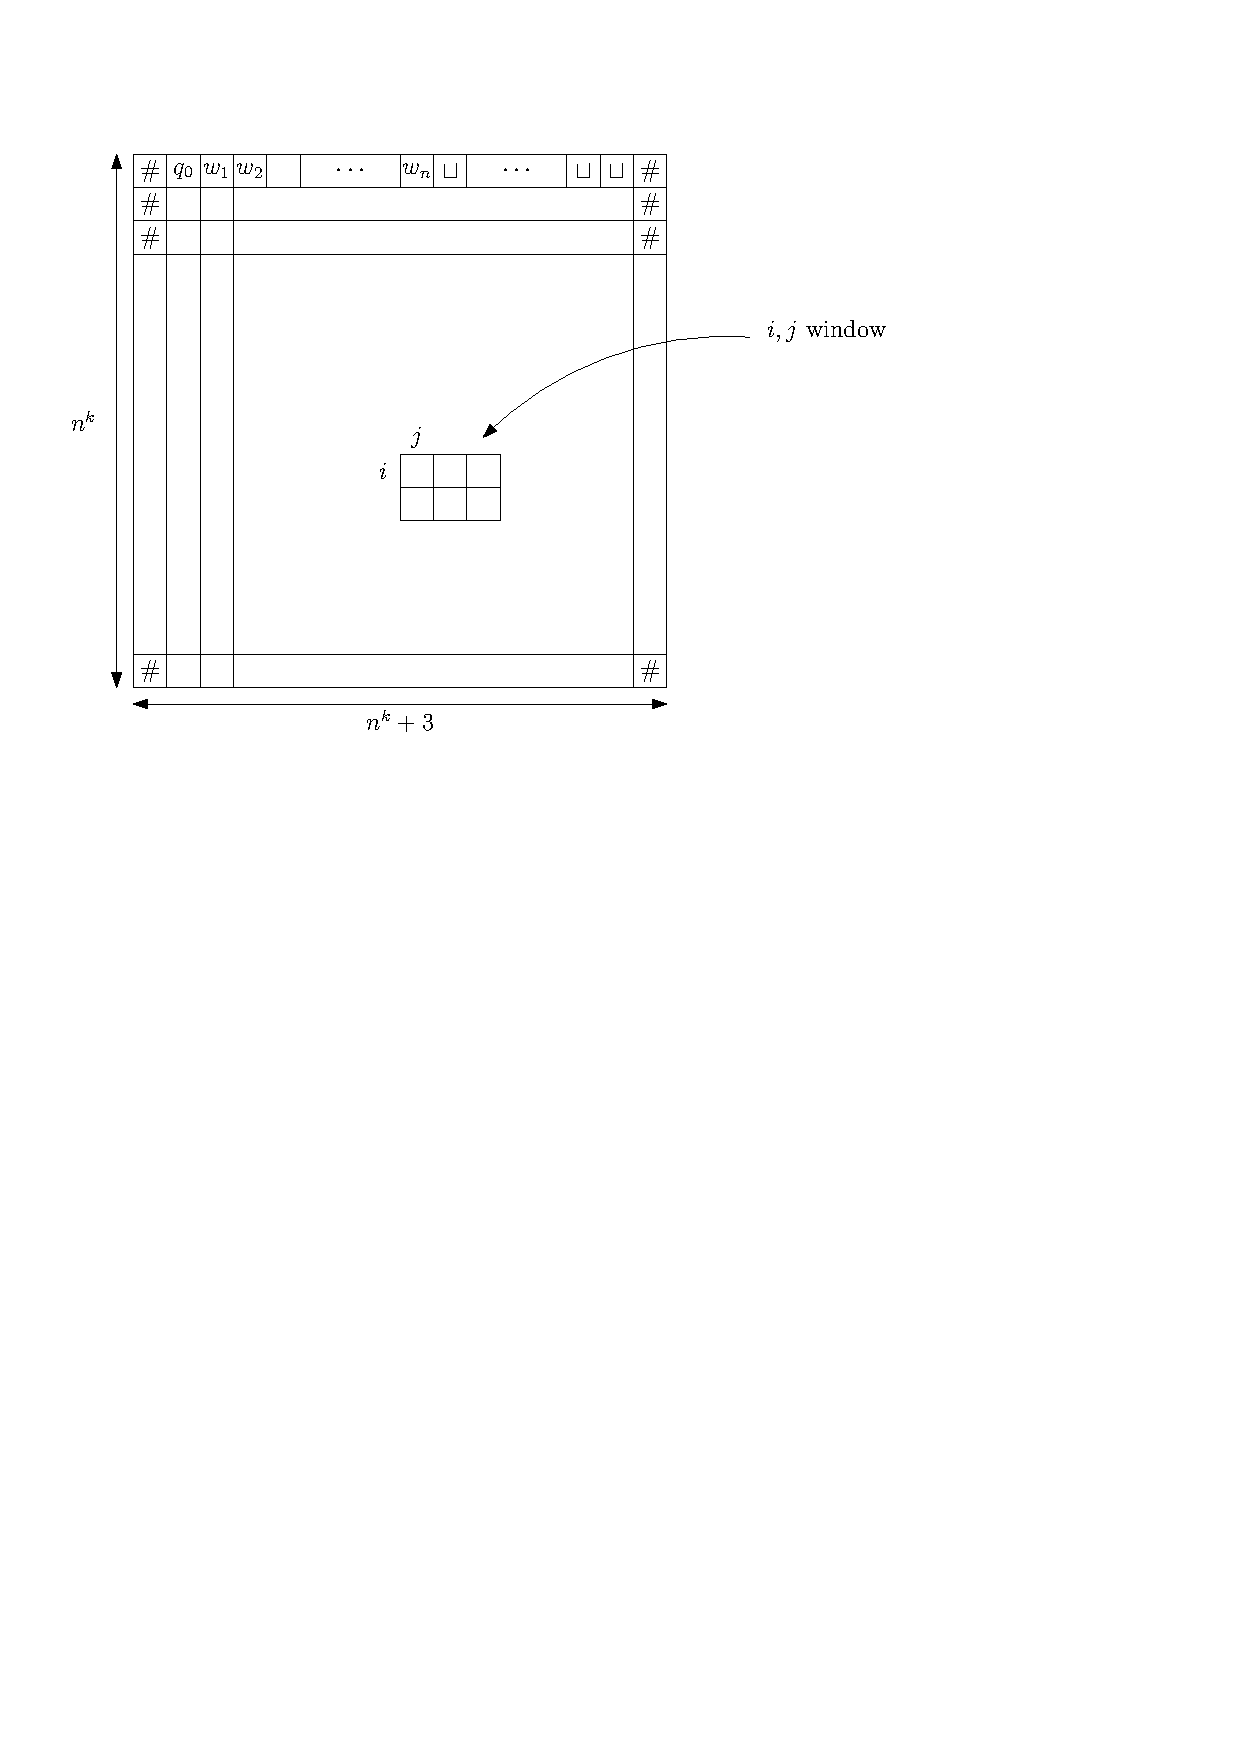
\includegraphics[width=0.7\linewidth]{tableau.pdf}
    \caption{A tableau.}
    \label{fig:cook-levin-tableau}
\end{figure}

Informally,
$$
\phi_{move} = \bigwedge_{\substack{1 \leq i \leq n^k - 1 \\ 1 \leq j \leq n^k + 1}} \left( \text{the $(i,j)$ window is legal} \right) 
$$
We express ``$(i,j)$ window is legal'' using the formula
$$
\bigvee_{\substack{(a_1,a_2,\ldots,a_6) \\ \text{is a legal window}}} \left( x_{i,j,a_1} \land x_{i,j+1,a_2} \land x_{i,j+2,a_3} \land x_{i+1,j,a_4} \land x_{i+1,j+1,a_5} \land x_{i+1,j+2,a_6} \right) 
$$
which is equivalent to
$$
\bigwedge_{\substack{(a_1,\ldots,a_6) \\ \text{isn't a legal window}}} \left( \overline{x_{i,j,a_1}} \lor \overline{x_{i,j+1,a_2}} \lor \overline{x_{i,j+2,a_3}} \lor \overline{x_{i+1,j,a_4}} \lor \overline{x_{i+1,j+1,a_5}} \lor \overline{x_{i+1,j+2,a_6}} \right) 
$$

\begin{figure}[htbp]
    \centering
    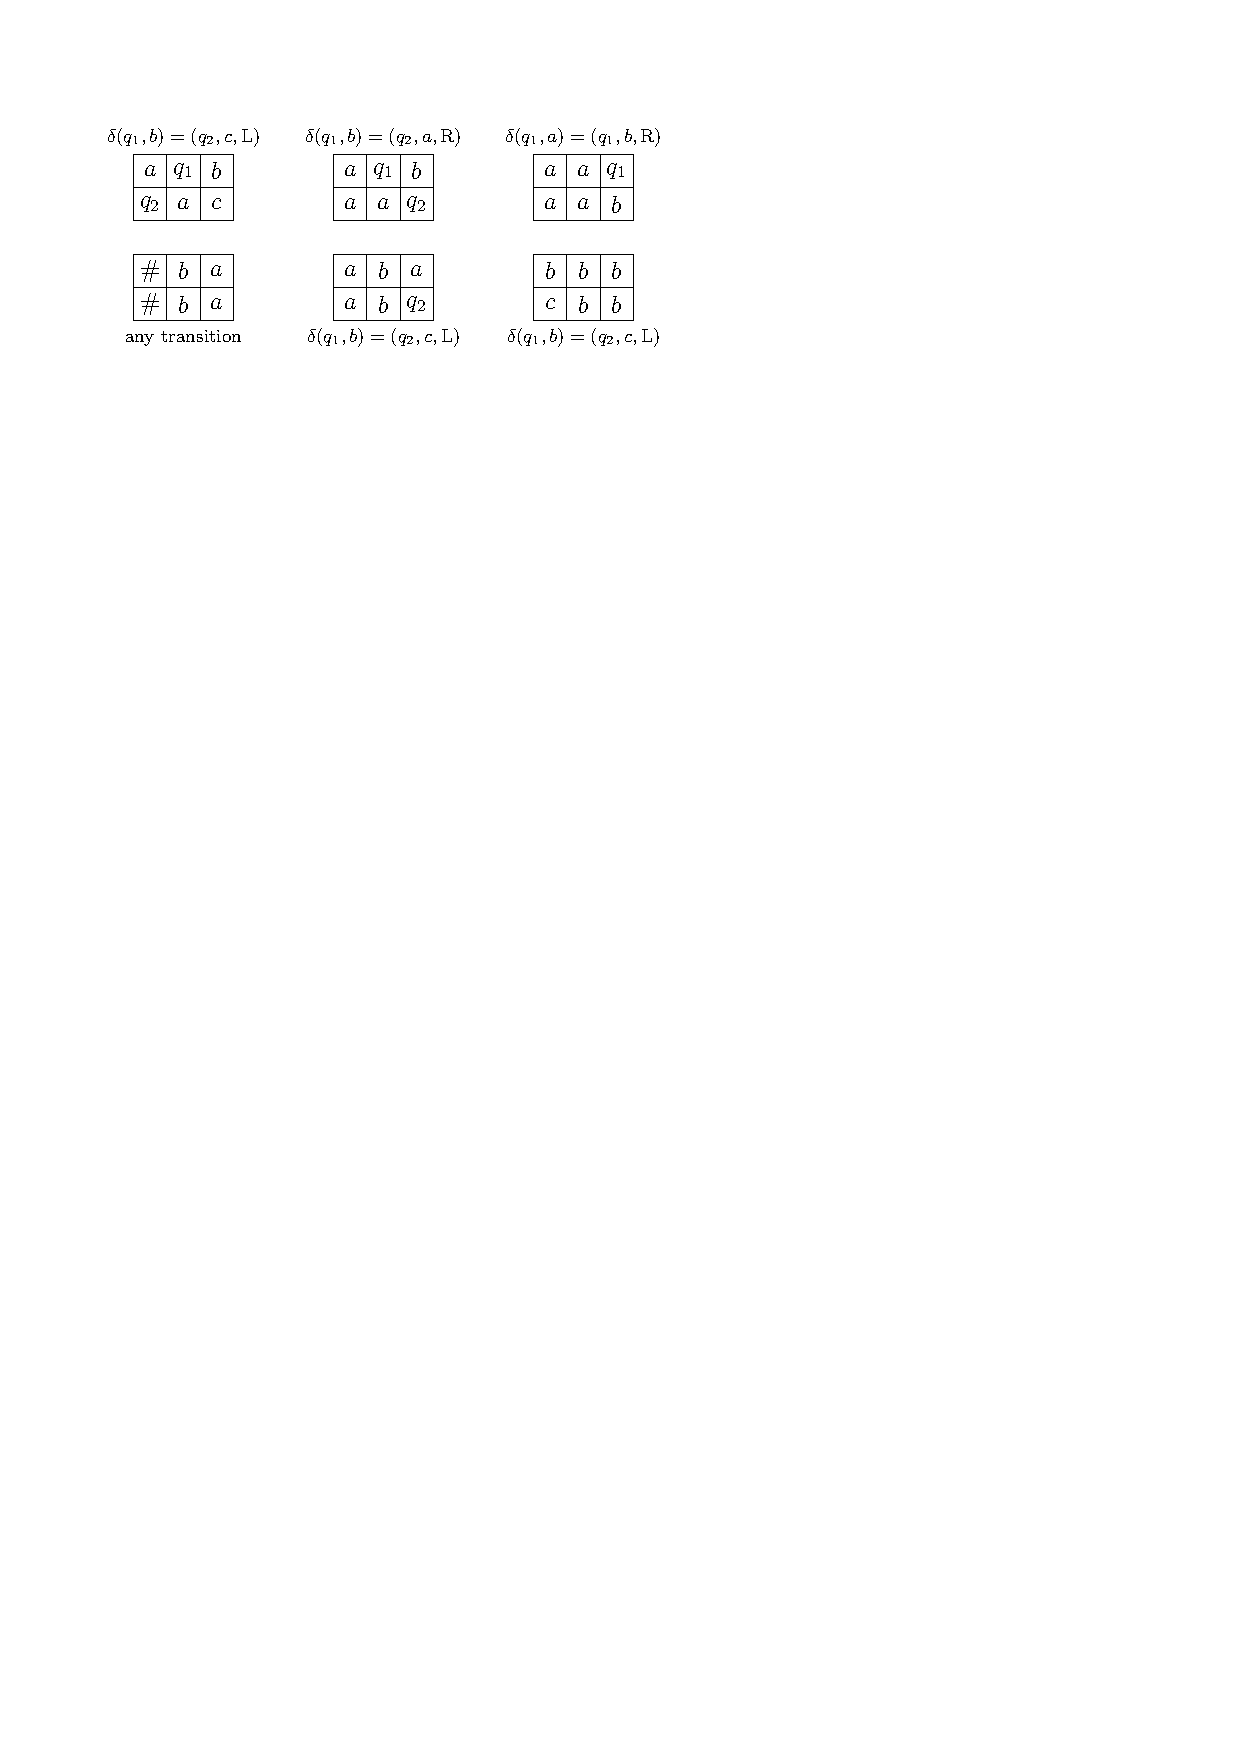
\includegraphics[width=0.6\linewidth]{legal-windows.pdf}
    \caption{Some legal windows under the transition function $\delta(q_1,b) = (q_2,c,\mathrm{L})$, $\delta(q_1,b) = (q_2,a,\mathrm{R})$, and $\delta(q_1,a) = (q_1,b,\mathrm{R})$.  }
    \label{fig:cook-levin-legal-windows}
\end{figure}

\begin{lemma}
    If the top row of the tableau is the start configuration and every window in the tableau is legal, each row of the tableau is a configuration that legally follows the preceding one. In other words, if some configuration does not follow from the previous one, we are guaranteed to detect the violation in some window.
\end{lemma}

\begin{proof}
    See Sipser Claim 7.41.
\end{proof}

Thus $A \leq_p \SAT$ so $\SAT$ is NP-complete.

\section{3SAT}

Everything is already in AND of ORs (CNF), we need to make this ORs small (3CNF). Let's start with a short example of a 4CNF with one clause.
$$
(a_1 \lor a_2 \lor a_3 \lor a_4) \iff (a_1 \lor a_2 \lor z_1) \land (\neg z_1 \lor a_3 \lor a_4)
$$
Every assignment that satisfies the formula on the LHS satisfies the formula on the RHS, and vice versa.

In general, for each clause in the original formula,
$$
(a_1 \lor a_2 \lor a_3 \lor \cdots \lor a_t)
$$
we can replace it with
$$
(a_1 \lor a_2 \lor z_1) \land (\neg z_1 \lor a_3 \lor z_2) \land (\neg z_2 \lor a_4 \lor z_3) \land (\neg z_3 \lor \cdots) \land \cdots \land (\neg z_{t-3} \lor a_{t-1} \lor a_{t})
$$
with $t-2$ clauses.

\chapter{NP-Complete Problems}
\section{Clique}

A clique in an undirected graph $G=(V,E)$ is sa set $S \subseteq V$ such that for all pairs of distinct $u, v \in S$, $\{u,v\} \in E$.

$$
\Clique = \{ \encoding{G,k} \mid \text{$G$ is a graph, $k \in \N$ and $G$ has a clique of size $k$ }\}
$$

\begin{theorem}
    CLIQUE is NP-compelte.
\end{theorem}

\begin{proof}
    Clearly, CLIQUQE $\in \NP$. To show that CLIQUE is NP-hard, we will show the reduction $\threeSAT \leq_p \Clique$.

    Given a 3CNF formula $\phi$, construct in polynomial time $\encoding{G_{\phi},k_{\phi}}$ such that
    $$
    \text{$\phi$ is satisfiable} \iff \text{$G_{\phi}$ has a clique of size $k$}
    $$
    Suppose $\phi = (a_1 \lor b_1 \lor c_1) \land (a_2 \lor b_2 \lor c_2) \lor \cdots \lor (a_k \lor b_k \lor c_k)$ with $k$ clauses and 3 literals per clause.

    We construct $G$ such that it has $k$ groups of 3 vertices (giving us $3k$ vertices) where each vertex is labeled according to a literal in a clause. We connect all pairs of vertices except:
    \begin{itemize}
        \item vertices in the same triple (same clause)
        \item vertices with contradictory labels ($x_i$ and $\overline{x_i}$)
    \end{itemize}
    Now assume that $\phi$ is satisfiable, then there exists some assignment of variables that satisfies $\phi$. Take such satisfying assignment. In this assignment, there must be at least one true literal in each clause. In each triple, pick any one vertex corresponding to the true literal. These vertices form a $k$-clique containing $k$ vertices, distinct triples (because there is no edge among vertices within the same triple), and no contradicting labels (becuase there is no edge between contradictory labels).

    Suppose a graph $G$ has a $k$-clique. Then, no two vertices in the clique are in the same triple. Each triple has exactly one vertex in the clique. Assign values to variables so that all clique nodes are true literals (this is possible since there is no contradictory labels in clique). This assignment satisfies $\phi$. Therefore, $\phi$ is satisfiable.
\end{proof}

Now consider the language $k$-CLIQUE. In this language, $k$ is fixed.
$$
\text{$k$-CLIQUE} = \{ \encoding{G} \mid \text{$G$ is an undirected graph with a clique of size $k$ }\}
$$
\begin{theorem}
    $k$-CLIQUE $\in \p$ for all $k$.
\end{theorem}

\begin{proof}
    Check all ${n \choose k}$ subset of vertices. Since $k$ is fixed, this number of subset needs be checked is polynomial in $n$.
\end{proof}

\section{Independent Sets}

$G=(V,E)$, $S \subseteq V$ is an independent set in $G$ if $\encoding{u,v}\not\in E$ for all distinct $u,v \in S$.

$$
\text{IND-SET} = \{\encoding{G,k} \mid \text{$G$ is a graph which contains an independent set of size $k$}\}
$$

\begin{theorem}
    IND-SET is NP-complete.
\end{theorem}

\begin{proof}
    We show that CLIQUE $\leq_p$ IND-SET.
\end{proof}

\section{Vertex Cover}

Let $G=(V,E)$ be an undirected graph. $S \subseteq V$ is a vertex cover for $G$ if every edge in $G$ has at least one endpoint in $S$.

$$
\text{VERTEX-COVER} = \{ \encoding{G,k} \mid \text{$G$ has vertex color of size $k$}\}
$$

\begin{theorem}
    VERTEX-COVER is NP-complete.
\end{theorem}

\begin{proof}
    Showing VERTEX-COVER $\in \NP$ is easy. We show VERTEX-COVER is NP-hard by showing
    $$
    \text{IND-SET} \leq_p \text{VERTEX-COVER}
    $$
    For the reduction, we map $\encoding{G,k}$ to $\encoding{G,|V|-k}$. We claim that $G=(V,E)$ where $S \subseteq V$ is an independent set in $G$ if and only if $V-S$ is a vertex cover.
\end{proof}

\section{Coloring}

An undirected graph $G$ is $k$-colorable if there is a map $f:\, V \to \{1,2\ldots,k\}$ such that for every edge $(u,v) \in E$, $f(u) \neq f(v)$.

\begin{theorem}
    2COL $\in \p$.
\end{theorem}

\begin{proof}
    Run BFS. Greedily assign colors by alternating coloring for each level.
\end{proof}

\begin{theorem}
    3COL is NP-complete.
\end{theorem}

\begin{proof}
    We show that 3SAT $\leq_p$ 3COL.

    \begin{figure}[htbp]
        \centering
        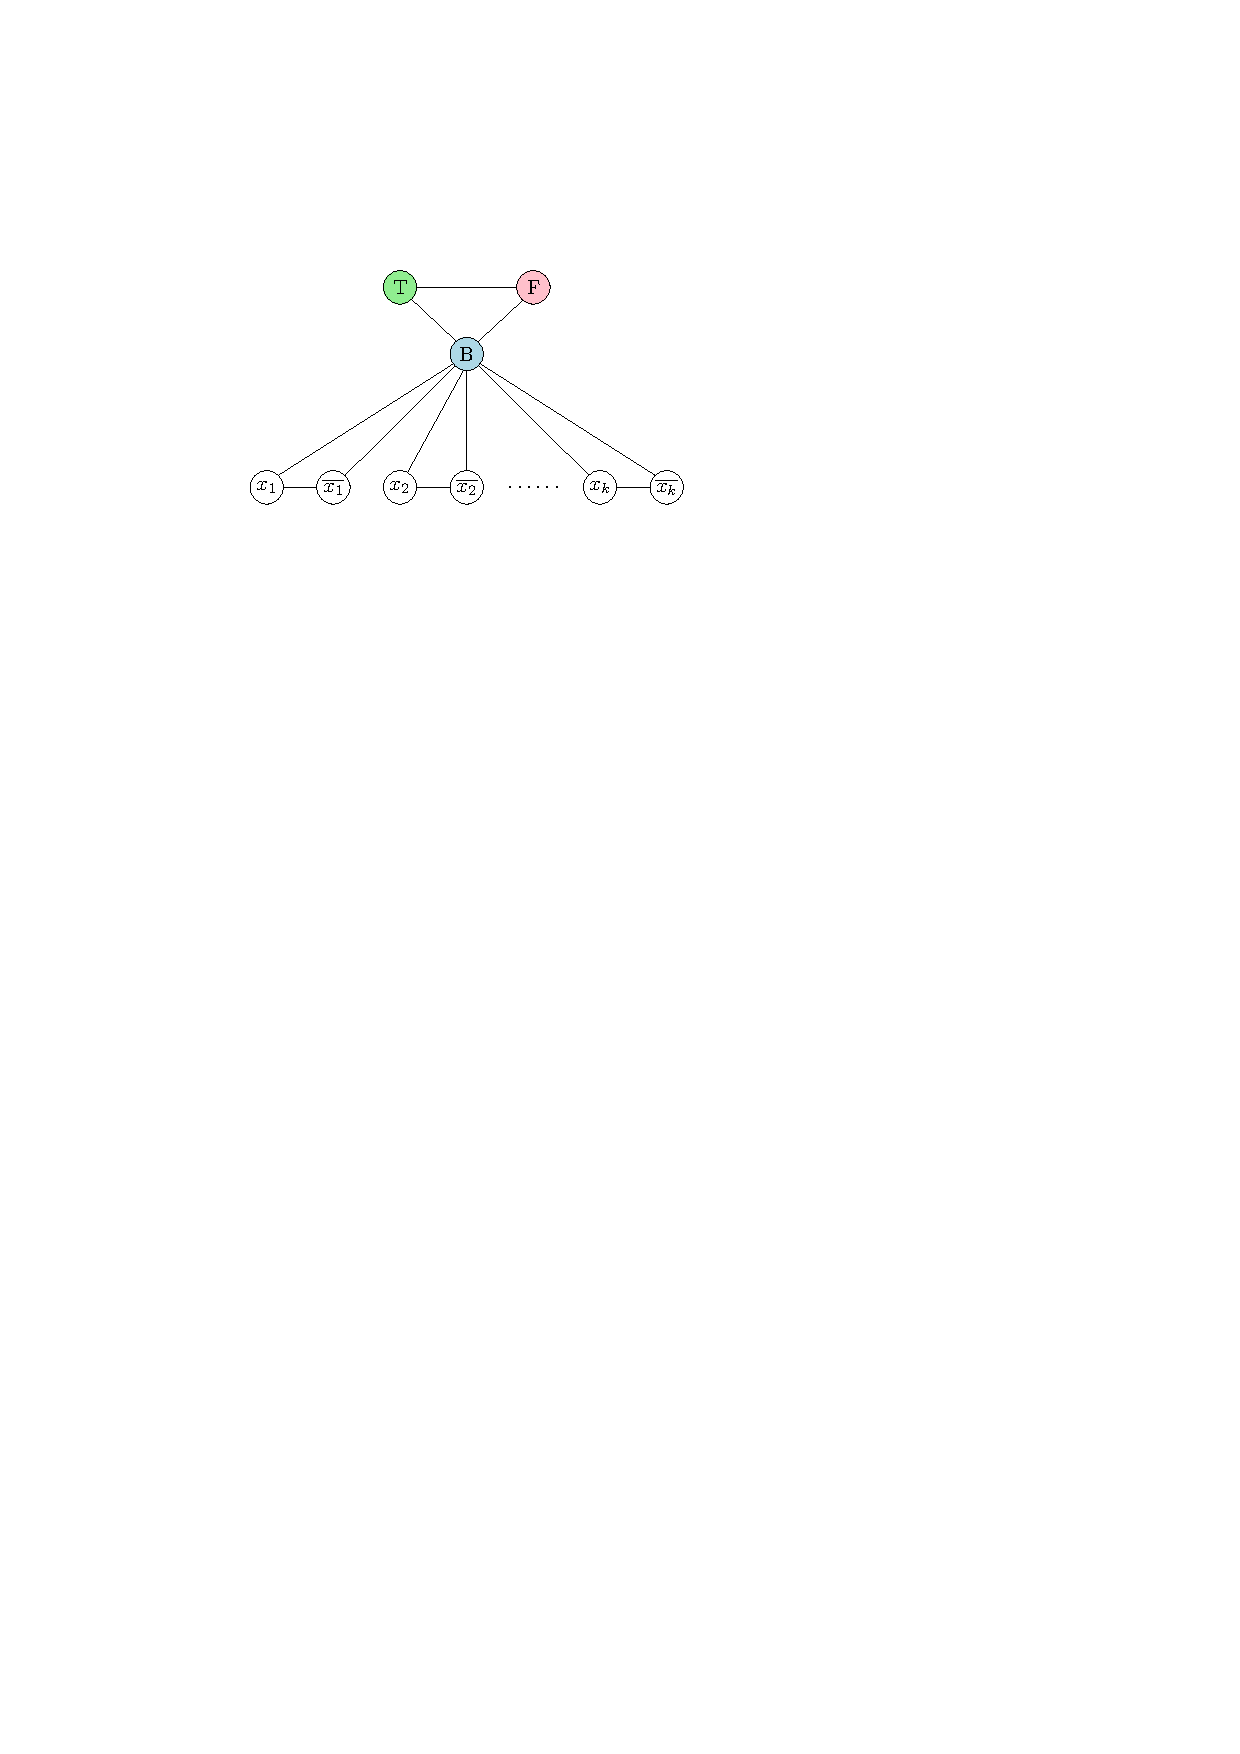
\includegraphics[width=0.4\linewidth]{3color-palette-variable-construction.pdf}
        \caption{Construction that ensures that a coloring corresponds to a valid truth assignment.}
        \label{fig:3color-valid-construction}
    \end{figure}

    \begin{figure}[htbp]
        \centering
        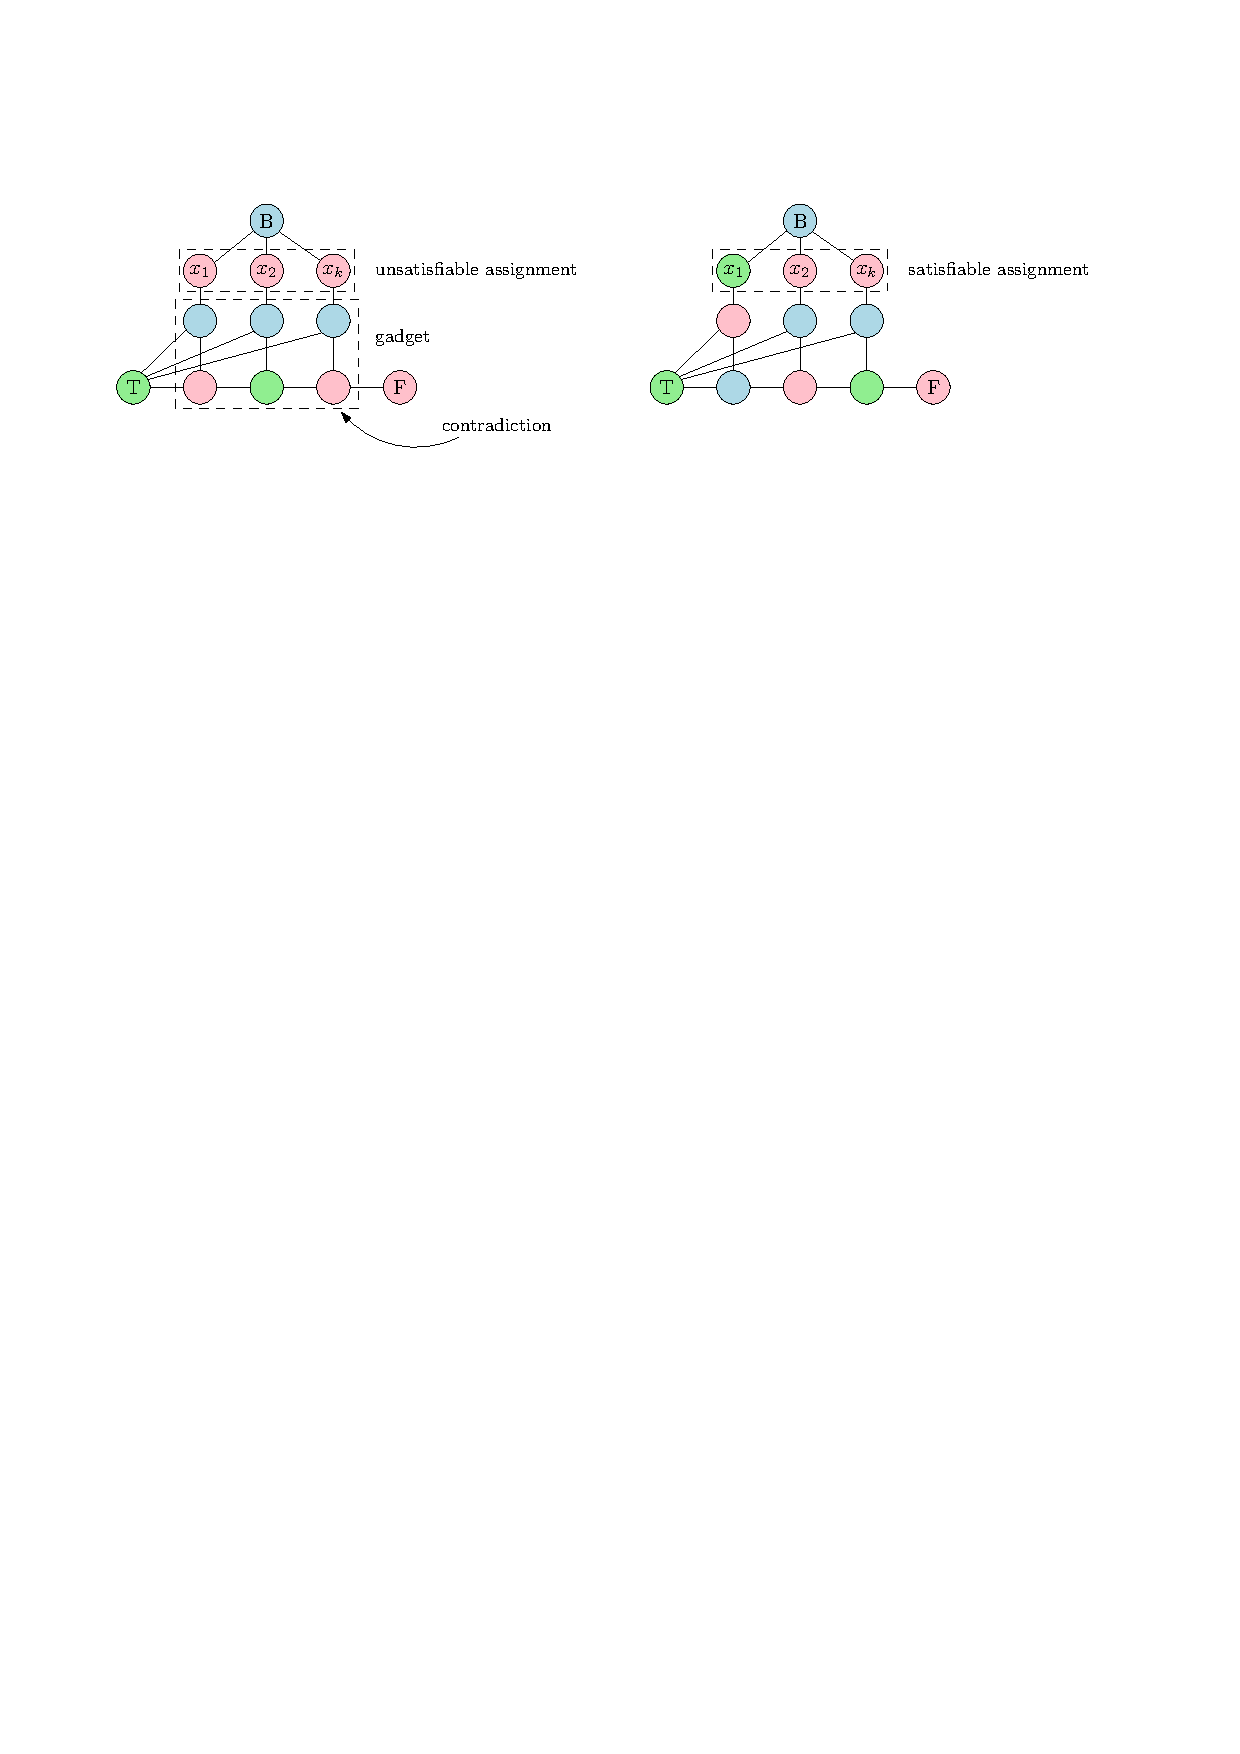
\includegraphics[width=0.8\linewidth]{3color-gadget-construction.pdf}
        \caption{Construction using gadgets that ensures only satisfiable truth assignment can be colored.}
        \label{fig:3color-gadgets-construction}
    \end{figure}

    An alternative construction uses the OR-gadget. The OR-gadget forces the three vertices within the gadget to have different colors. This, in turn, forces a contradiction at the output gadget when we have all literals being false.

    \begin{figure}[htbp]
        \centering
        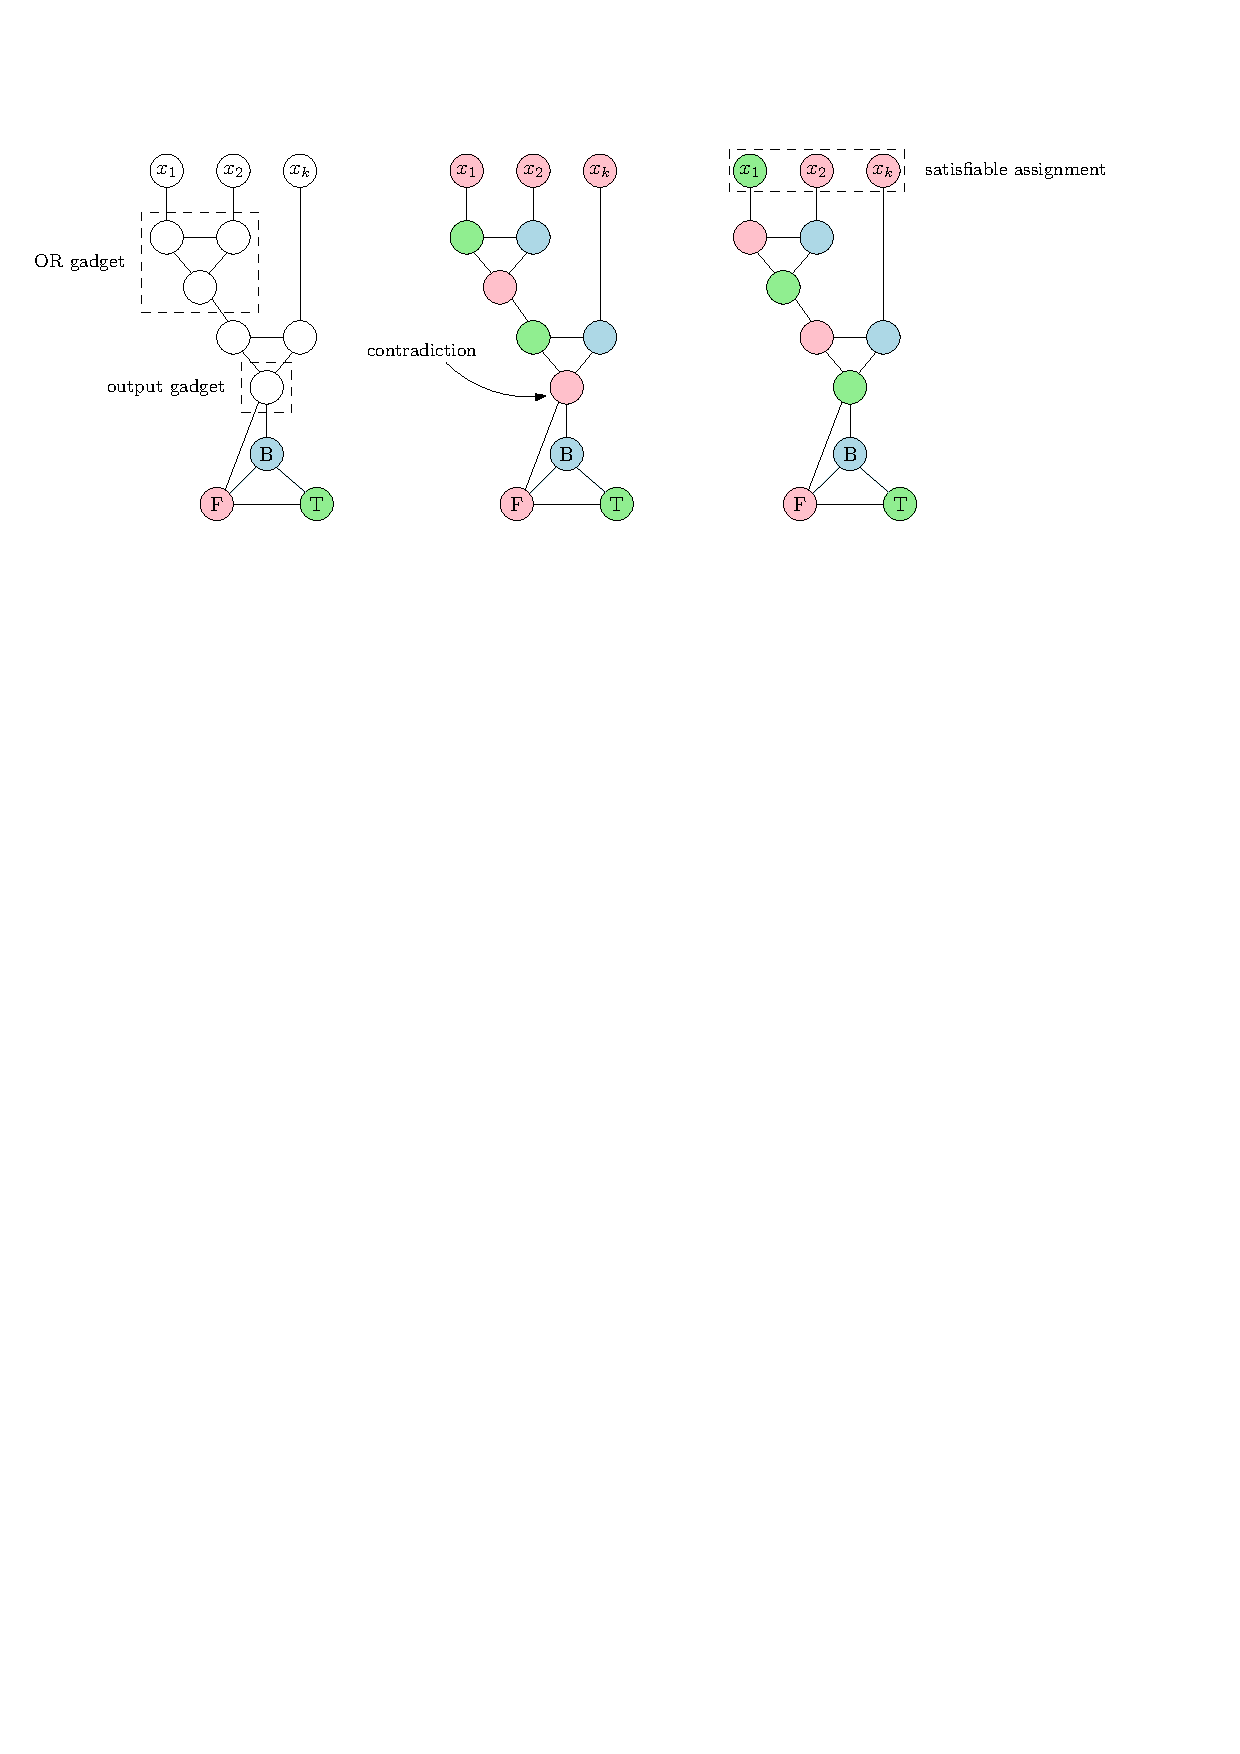
\includegraphics[width=0.9\linewidth]{3color-gadget-alternative-construction.pdf}
        \caption{Construction using gadgets that ensures only satisfiable truth assignment can be colored.}
        \label{fig:3color-gadgets-alternative-construction}
    \end{figure}
\end{proof}

\section{Subset Sum}

Given a collection of numbers $x_1,\ldots,x_k$ and a target $t$, is there a subcollection adding up to $t$.
$$
\text{SUBSET-SUM} = \{\encoding{s,t} \mid \text{$s = \{x_1,\ldots,x_k\}$ and for some $\{y_1,\ldots,y_i\} \subseteq \{x_1,\ldots,x_k\}$, $\Sigma y_i = t$}\}
$$

\begin{proof}
    
\end{proof}

\chapter{Space Complexity}
\section{Space Complexity}

We define the space complexity as the largest tape index reached during the computation.

\begin{definition}[Space Complexity]
    The space complexity of $M$ is the function $f:\, \N \to \N$ where $f(n)$ is the largesttape index reached by $M$ on any input of length $n$.
\end{definition}

\begin{definition}[Space Complexity Class]
     $$
     \Space(f(n)) = \{ L \mid \text{$L$ is decided by a TM with $O(f(n))$ space complexity}\}
     $$ 
\end{definition}

\begin{theorem}
    $
    \text{3SAT} \in \Space(n)
    $
\end{theorem}

\begin{proof}
    Given 3SAT formula $\phi$ of length $n$, try all possible assignments to at most $n$ variables. Evaluate $\phi$ on each assignment. Accept if and only if there is a satisfying assignment. This can be carried out in $O(n)$ space.
\end{proof}

\begin{theorem}
    $
    \NTime(t(n)) \subseteq \Space(t(n))
    $
\end{theorem}

\begin{definition}[PSPACE]
    $$
    \PSpace = \bigcup_{k \in \N} \Space(n^k)
    $$
\end{definition}

$\PSpace$ formalizes problems solvable by computers with bounded memory. $\PSpace$ is more general because we can reuse space.

Open question: $\p \overset{?}{=} \PSpace$

If $\p = \PSpace$, then $\p = \NP$. 

\section{Time Complexity of SPACE}

Let $M$ be a Turing machine that halts with space complexity $f(n)$. How many steps could $M$ take on inputs of length $n$?

Number of steps is at most number of possible configurations. Recall that a configuration encodes the head position, state, $f(n)$ cells of tape content, so the length of a configuration is in $O(f(n))$. It follows that the total number of configurations is in $O(2^{f(n)})$.

Hence,
$$
\PSpace \subseteq \ExpTime
$$

So far, we have
$$
\p \subseteq \NP \subseteq \PSpace \subseteq \ExpTime
$$

\begin{theorem}
    $
    \p \neq \ExpTime
    $
\end{theorem}

\begin{proof}
    By the time hierarchy theorem.
\end{proof}

So, at least one of $\p \neq \NP$ and $\NP \neq \PSpace$ and $\PSpace \neq \ExpTime$ must be true.

\section{Nondeterministic Space}

\begin{definition}[NSPACE]
    $$
    \NSpace(f(n)) = \{ L \mid \text{$L$ is decided by a nondeterministic TM with $O(f(n))$ space complexity}\}
    $$
\end{definition}

\begin{definition}[NPSPACE]
    $$
    \NPSpace = \bigcup_{k \in \N} \NSpace(n^k)
    $$
\end{definition}

\section{Savitch's Theorem}

\begin{theorem}[Savitch's Theorem]
    For any function $f:\,\N \to \R^+$ where $f(n) \geq n$,
    $$
    \NSpace(f(n)) \subseteq \Space(f^2(n))
    $$
\end{theorem}

\begin{proof}
    Let $N = (Q,\Sigma,\Gamma, \delta, q_0, q_{acc}, q_{rej})$ be NTM with space complexity $f(n)$. We will construct a DTM $M$ with space complexity $O(f^2(n))$ such that $\lang(M) = \lang(N)$.

    Let $w \in \Sigma^n$ be input of length $n$. We define a directed graph $G = (V,E)$ called $f(n)$ space configuration graph of $N$ where
    $$
    V = \{\text{configurations of $N$ with at most $f(n)$ }\}
    $$

    Observe that $w \in \lang(N)$ if and only if there exists a path in $G$ of length at most $2^{d f(n)}$ from $q_0w$ to an accepting configuration of the form $xq_{acc}y$.

    \begin{codebox}
        \Procname{$\proc{Can-Yield}(c_1,c_2,t)$}
        \li \If $t \isequal 1$ \Then
            \li \If $c_1$ yields $c_2$ \Then
                \li \textbf{accept}
            \li \Else \textbf{reject}
            \End
        \End
        \li \If $t \geq 2$ \Then
            \li \For $c_3 \in V$ in order \Do
                \li $\proc{Can-Yield}(c_1,c_3,\lceil t/2 \rceil )$ 
                \li $\proc{Can-Yield}(c_3,c_2,\lfloor t/2 \rfloor )$
                \li \If both accept for some $c_3$ \Then
                    \li \textbf{accept}
                \li \Else \textbf{reject}
    \end{codebox}

\begin{turing}{M}{on input $w$ of length $n$}
    \item \textbf{for each} $c \in V$ in orders
    \item \qquad \textbf{if} $c$ is an accepting configuration
    \item \qquad \qquad run $\proc{Can-Yield}(q_0w, c, 2^{df(n)})$ 
    \item \qquad \qquad \textbf{if} it accepts then \textbf{accept}
    \item \qquad \qquad \textbf{else} \textbf{continue}
    \item \qquad \textbf{if} $\proc{Can-Yield}(q_0w, c, 2^{df(n)})$ rejects for every accepting configuration $c \in V$, \textbf{reject}
\end{turing}

\end{proof}

Thus, by Savitch's theorem
$$
\PSpace = \NPSpace
$$
We can simulate any $\NPSpace$ Turing machine using a deterministic TM with only a quadratic overhead.

\section{PSPACE-Complete}

\begin{definition}[PSPACE-Complete]
    Language $B$ is $\PSpace$-complete if
    \begin{enumerate}
        \item $B$ is in $\PSpace$
        \item Every $A$ in $\PSpace$ is \textbf{poly-time} reducible to $B$ (i.e. $B$ is $\PSpace$-hard)
    \end{enumerate}
\end{definition}

\begin{theorem}
    If $B$ is $\PSpace$-complete and $B$ is in $\p$, then $\p = \PSpace$.
\end{theorem}

\begin{proof}[Proof idea]
    Let $A \in \PSpace$. The poly-time TM for $A$ first reduces input $x$ to an instance $y$ of $B$. Then it runs the polytime TM for $B$ on $y$ and outputs the answer.
\end{proof}

\begin{theorem}
    If $B$ is $\NPSpace$-complete and $B$ is in $\NP$, then $\NP = \PSpace$.
\end{theorem}

\subsection{TQBF}

\vspace{\parskip}

\begin{definition}[Fully Quantified Boolean Formula]
    A \textit{\textbf{fully quantified Boolean formula}} is a Boolean formula where every variable in the formula is quantified ($\exists$ or $\forall$). If all quantifiers appear at the beginning of the statement and that each quantifier's scope is everything following it, we say the statement is in \textit{\textbf{prenex normal form}} (PNF).
\end{definition}

$$
\text{TQBF} = \{\encoding{\phi} \mid \text{$\phi$ is a true fully quantified Boolean formula}\}
$$

\begin{theorem}
    TQBF is $\PSpace$-complete.
\end{theorem}

Note that SAT is a special case where all quantifiers are $\exists$. And TAUT is a special case where all quantifiers are $\forall$.

TAUT is a special case where all quantifiers are $\forall$. So clearly, SAT $\leq_p$ TQBF and TAUT $\leq_p$ TQBF.

\begin{theorem}[Meyer-Stockmeyer]
    TQBF is $\PSpace$-complete.
\end{theorem}

\begin{proof}
    We need to show two things: (1) TQBF is in $\PSpace$; and (2) TQBF is $\PSpace$-hard.

    We show that TQBF $\in \PSpace$. Consider the Turing machine $T$ that decides TQBF.

    \begin{turing}{T}{on input $\encoding{\phi}$}
        \item if $\phi$ has no quantifiers, evaluate $\phi$. Accept if it evaluates to 1.
        \item If $\phi = \exists x.\, \psi$, recursively call $T$ on $\psi$, first with $x=0$ and then $x=1$. If either result is accept, then accept; otherwise reject.
        \item If $\phi = \forall x.\, \psi$, recursively call $T$ on $\psi$ first with $x=0$ and then $x=1$. If both results are accept, then accept; otherwise reject.
    \end{turing}

    Note that we can reuse space. The depth of recursion is number of variables. At each level, we just need to store value of one variable. Hence, the space used is in $O(m)$ where $m$ is the number of variables.

    To show that TQBF is $\PSpace$-hard, we show that for all $A \in \PSpace$, $A \leq_p$ TQBF.

    For every $A \in \PSpace$, there exists some constant $k$ and Turing machine $M$ that decides $A$ in space of at most $n^k$. However, $M$ may run exponentially many steps, so simply encoding the computation history tableau directly won't work because we cannot construct an exponentially-sized formula in polynomial time.

    Fix $M$ and $w$, we will construct a quantified Boolean formula $\phi$ such that $\text{$M$ accepts $w$} \iff \text{$\phi$ is true}$. We will actually show how to construct $\phi_{c_1,c_2,t}$ to be a formula that is true if and only if $M$ can go from configuration $c_1$ and $c_2$ in at most $t$ steps. Note that in the construction that follows, $c_1,c_2,m_1$ are not necessarily one single variable, but collections of variables that represent some configurations. We can encode a configuration using $l \in O(n^k)$ variables from the proof of Cook-Levin's theorem.

    When $t=1$, it is easy to construct $\phi_{c_1,c_2,1}$. This translates to ``$c_2$ follows from $c_1$''. This is essentially the same construction used in the proof of Cook-Levin theorem.

    When $t > 1$, we construct $\phi_{c_1,c_2,t}$ recursively.
    $$
    \phi_{c_1,c_2,t} = \exists m_1.\, [\phi_{c_1,m_1,t/2} \land \phi_{m_1,c_2,t/2}]
    $$
    where $m_1$ represents variables describing a configuration of $M$. Notice, however, at each stage, the size of the formula doubles. This will lead to an exponential explosion of the size of the formula. In the end, we would have a formula of size in the order of $t = 2^{dn^k}$.

    Instead, we use a clever construction:
    $$
    \phi_{c_1,c_2,t} = \exists m_1.\, \forall c_3,c_4.\, [ (c_3,c_4) = (c_1,m_1) \lor (c_3,c_4) = (m_1,c_2) \implies \phi_{c_3,c_4,t/2} ]
    $$
    This construction essentially says: ``for all variables $c_3,c_4$ encoding a configuration, if $c_3,c_4$ represents $c_1,m_1$, then $\phi_{c_3,c_4,t/2}$ must be true; and the same is true for the case when $c_3,c_4$ represents $c_1,m_1$''.

    With this construction, the size of the formula increases at most by an additive factor of size $O(n^k)$. At the end, following the recursive construction described as above, we have 
    $$
    \phi_{c_{start},c_{end},2^{d^{n^k}}}
    $$
    The level of recursion is $\log(2^{dn^k})$ and each level of recursion adds a portion of the formula with size linear in the size of the variables encoding a configuration, which is in $O(n^k)$. Therefore, in the end, the size of the formula is $O(n^{2k})$, polynomial in the input size.
\end{proof}

\chapter{The Class L and NL}
\section{L and NL}

Sublinear space bounds where $f(n)$ is much smaller than $n$. This won't make sense given our existing one-tape Turing machine model since we won't even have enough space to store the input.

We modify our model and have a 2-tape Turing machine where we have one tape as a read-only input tape, and another tape as the read/write work tape. We don't have to store all data on the main memory, so we would like to consider \textit{only the computation spaced used on the work tape}.

$$
\LSpace = \Space(\log n)
$$
$$
\NLSpace = \NSpace(\log n)
$$

Savitch's theorem still holds, so $\NLSpace \subseteq \Space(\log^2 n)$.

\section{PATH is in NL}

$$
\text{PATH} = \{ \encoding{G,s,t} \mid \text{$G$ has directed path from $s$ to $t$ } \}
$$

\begin{theorem}[PATH in NL]
    $$
    \text{PATH} \in \NLSpace
    $$
\end{theorem}

\begin{proof}
    At each vertex, we use nondeterminism to guess the next vertex. Suppose we have the path $p = s s_1 s_2 \ldots t$. At each vertex $s_i$, we look at the next vertex $s_{i+1}$ and checks if $s_{i+1}$ is connected to $s_i$. If any of the nondeterministic paths lead to $t$. At any time during the computation of one nondeterministic path, we have at most the name of two vertices on the work tape. In addition, we keep track of the vertices visited, using $\log n$ space since any simple path contains at most $n$ vertices. It takes at most $\log n$ space to write down the name of a vertex, so PATH $\in \NLSpace$.
\end{proof}

We do not know if PATH $\overset{?}{\in} \LSpace$. We also don't know if $\LSpace \overset{?}{=} \NLSpace$.

\section{NL-Complete}

A language $A$ is in $\NLSpace$-complete if $A \in \NLSpace$ and for all $B \in \NLSpace$, $B \leq_L A$. The symbol $\leq_L$ stands for log-space reducible, which we will define here.

All problems in $\NLSpace$ are also in $\p$.
$$
\NLSpace \subseteq \p
$$
For all $A,B \in \NLSpace$ except $\emptyset$ and $\Sigma^*$, $A \leq_p B$ and $B \leq_p A$.

\subsection{Log-Space Reduction}

A log-space transducer is a Turing machine with
\begin{itemize}
    \item read-only input tape
    \item write-only output tape (head can only move to the right)
    \item read/write work tape (only $O(\log n)$ symbols)
\end{itemize}
that computes a function $f:\; \Sigma^* \to \Sigma^*$ where $f(w)$ is written on output tape when $M$ halts when $w$ is on the input tape.

We say $f$ is a log-space computable function.

\begin{theorem}
    if $A \leq_L B$ and $B \in \LSpace$, then $A \in \LSpace$.
\end{theorem}

\begin{proof}
    Suppose there exists a log-space decider $M_B$ for $B$. We construct a log-space decider for $A$.

    \begin{turing}{M}{on input $w$}
        \item run $w$ on the log-space transducer to compute $f(w)$ 
        \item run $M_B$ on $f(w)$ 
    \end{turing}

    The issue with this construction is that we don't have enough space to actually write down the entirety of $f(w)$, so this construction won't quite work.

    We use this algernative construction. Whenever $B$ needs a bit of $f(w)$, we recompute it on the fly. More formally, $M_A$ computes individual symbols of $f(w)$ by calling the logspace transducer as requested by $M_B$. In the simulation, we run $M_B$ without actual input on the tape. When it requests the $i$th bit of the input, we run $M_A$ with a counter to get the $i$th bit of $f(w)$.

    To see why this construction of $M_A$ runs in logspace, observe first that $M_A$ itself needs to keep track of the position requested by $M_B$ when calling the transducer, which takes $O(\log n)$ space. In addition, $M_B$ uses $O(\log |f(w)|) + 1$ space (the one additional bit is used to store the bit requested by $M_B$ at each step of its computation) when we simulate $M_B$. Since $f(w)$ has length of as most the number of configurations that the transducer can have, which is $|w| 2^{O(\log |w|)}$. It follows that the space used by $M_B$ is also in $O(\log |w|) = O(\log n)$. Therefore, $M_A$ runs in logspace.
\end{proof}

\subsection{PATH is NL-Complete}

\vspace{\parskip}

\begin{theorem}
    PATH is $\NLSpace$-complete.
\end{theorem}

\begin{proof}
    We have shown that PATH is in $\NLSpace$. It reamins to be shown that for every language $A \in \NLSpace$, $A \leq_L$ PATH.

    Let $A \in \NLSpace$. There exists a nondeterministic log-space Turing machine $M$ that decides $A$. Given a string $w$, we want to reduce it to a graph representing the computation of $M$ on $w$ where:
    \begin{itemize}
        \item nodes: various configurations
        \item edges: $(c_1,c_2) \in E$ if $c_1$ yields $y_2$  
    \end{itemize}
    Why is this construction log-space computable? We need to give a log-space transducer that outputs $\encoding{G,s,t}$ on input $w$. Note that when constructing a log-space transducer, we don't actually care about the time complexity of the transducer, although the construction that we are about to show is both log-space and runs in polytime. The transducer needs to do two things:

    \begin{enumerate}
        \item List the nodes: This is relatively easy. Each node is a configuration of $M$ on $w$ which can be represented in $c \log n$ space for some constant $c$. The transducer can simply go through every strings of length $c \log n$ using brute force, checks if it encodes a legal configuration of $M$ on $w$, and outputs those that do. This runs in log-space because at any time, we only write at most one string on the work tape.
        \item List the edges: We list the edges of the graph by testing every pair of possible configurations $(c_1,c_2)$ and checks if $c_1$ yields $c_2$. This can be done using log-space as well because we only need to write $c_1$, $c_2$ on the work tape while looking at the transition table to determine if $c_1$ yields $c_2$.
    \end{enumerate}
\end{proof}

\begin{corollary}
    $$
    \NLSpace \subseteq \p
    $$
\end{corollary}

\begin{proof}
    A Turing machine that uses space $f(n)$ runs in time $n 2^{O(f(n))}$, so a reducer that runs in log-space also runs in polynomial time. Therefore, any language in $\NLSpace$ is polynomial time reducible to PATH, which is in $\p$.
\end{proof}

%----------------------------------------------------------------------------------------
%	APPENDIX
%----------------------------------------------------------------------------------------
\part*{Appendix}
\appendix
\chapter*{Commonly Used Axioms \& Theorems}
\addcontentsline{toc}{chapter}{\textcolor{ocre}{Axioms \& Theorems}} 

\renewcommand{\leftmark}{\sffamily\bfseries Axioms \& Theorems}
\renewcommand{\rightmark}{\sffamily\bfseries Axioms \& Theorems}

\section*{Rules of Inference} \label{rulesofinference}

\begin{axiom_appendix}[Modus Ponens]
$(P \wedge (P \implies Q)) \implies Q $
\end{axiom_appendix}

\begin{axiom_appendix}[Modus Tollens]
$(\neg Q \wedge (P \implies Q)) \implies \neg P $
\end{axiom_appendix}

\begin{axiom_appendix}[Hypothetical Syllogism (transitivity)]
\hfill

$((P \implies Q) \wedge (Q \implies R)) \implies (P \implies R) $
\end{axiom_appendix}

\begin{axiom_appendix}[Disjunctive Syllogism]
$((P \vee Q) \wedge \neg P) \implies Q$
\end{axiom_appendix}

\begin{axiom_appendix}[Addition]
$P \implies (P \vee Q)$
\end{axiom_appendix}

\begin{axiom_appendix}[Simplification]
$(P \wedge Q) \implies P$
\end{axiom_appendix}

\begin{axiom_appendix}[Conjunction]
$((P) \wedge (Q)) \implies (P \wedge Q)$
\end{axiom_appendix}

\begin{axiom_appendix}[Resolution]
$((P \vee Q) \wedge (\neg P \vee R)) \implies (Q \vee R)$
\end{axiom_appendix}

\section*{Laws of Logic}

\begin{axiom_appendix}[Implication Law]
$(P \implies Q) \equiv (\neg P \vee Q)$
\end{axiom_appendix}

\begin{axiom_appendix}[Distributive Law]
\begin{align*}
    (P \wedge (Q \vee R)) &\equiv ((P \wedge Q) \vee (P \wedge R)) \\
    (P \vee (Q \wedge R)) &\equiv ((P \vee Q) \wedge (P \vee R))
\end{align*}
\end{axiom_appendix}

\begin{axiom_appendix}[De Morgan's Law]
\begin{align*}
    \neg (P \wedge Q) &\equiv (\neg P \vee \neg Q) \\
    \neg (P \vee Q) &\equiv (\neg P \wedge \neg Q)
\end{align*}
\end{axiom_appendix}

\begin{axiom_appendix}[Absorption Law]
\begin{align*}
    (P \vee (P \wedge Q)) &\equiv P \\
    (P \wedge (P \vee Q)) &\equiv P
\end{align*}
\end{axiom_appendix}

\begin{axiom_appendix}[Commutativity of AND]
$A \wedge B \equiv B \wedge A$
\end{axiom_appendix}

\begin{axiom_appendix}[Associativity of AND]
$(A \wedge B) \wedge C \equiv A \wedge (B \wedge C)$
\end{axiom_appendix}

\begin{axiom_appendix}[Identity of AND]
$\textbf{T} \wedge A \equiv A$
\end{axiom_appendix}

\begin{axiom_appendix}[Zero of AND]
$\textbf{F} \wedge A \equiv \textbf{F}$
\end{axiom_appendix}

\begin{axiom_appendix}[Idempotence for AND]
$A \wedge A \equiv A$
\end{axiom_appendix}

\begin{axiom_appendix}[Contradiction for AND]
$A \wedge \neg A \equiv \textbf{F}$
\end{axiom_appendix}

\begin{axiom_appendix}[Double Negation]
$\neg (\neg A) \equiv A$
\end{axiom_appendix}

\begin{axiom_appendix}[Validity for OR]
$A \vee \neg A \equiv \textbf{T}$
\end{axiom_appendix}

\section*{Induction}

\vspace{\parskip}

\begin{axiom_appendix}[Well Ordering Principle]
Every nonempty set of nonnegative integers has a smallest element. i.e., For any $A \subset \N$ such that $A \neq \emptyset$, there is some $a \in A$ such that $\forall a' \in A.a\leq a'$.
\end{axiom_appendix}

\section*{Recurrences}

\vspace{\parskip}

\begin{theorem_appendix}[The Master Theorem]
Suppose that for $n \in \Z^+$.
\begin{equation*}
    T(n) =
    \begin{cases}
    c & \text{if $n<B$} \\
    a_1 T(\lceil n/b \rceil) + a_2 T(\lfloor n/b \rfloor) + dn^i & \text{if $n\geq B$}
    \end{cases}
\end{equation*}
where $a_1, a_2, B, b \in \N$.

Let $a = a_1+a_2 \geq 1$, $b>1$, and $c,d,i \in \R \cup \{0\}$. Then,
\begin{equation*}
    T(n) \in
    \begin{cases}
    O(n^i \log n) & \text{if $a=b^i$} \\
    O(n^i) & \text{if $a < b^i$} \\
    O(n^{\log_b a}) & \text{if $a > b^i$}
    \end{cases}
\end{equation*}
\end{theorem_appendix}

Linear Recurrences:

A linear recurrence is an equation
$$
f(n) = \underbrace{a_1 f(n-1) + a_2 f(n-2) + \cdots + a_d f(n-d)}_{\text{homogeneous part}}  + \underbrace{g(n)}_{\text{inhomogeneous part}}
$$
along with some boundary conditions.

The procedure for solving linear recurrences are as follows:

\begin{enumerate}
    \item Find the roots of the characteristic equation. Linear recurrences usually have exponential solutions (such as $x^n$). Such solution is called the \textbf{homogeneous solution}.
    $$
    x^n = a_1 x^{n-1} + a_2 x^{n-2} + \cdots + a_{k-1} x + a_k
    $$
    \item Write down the homogeneous solution. Each root generates one term and the homogeneous solution is their sum. A non-repeated root $r$ generates the term $cr^n$, where $c$ is a constant to be determined later. A root with $r$ with multiplicity $k$ generates the terms
    $$
    d_1r^n \quad d_2nr^n \quad d_3n^2r^n \quad \cdots \quad d_kn^{k-1}r^n
    $$
    where $d_1,\cdots,d_k$ are constants to be determined later.
    \item Find a \textbf{particular solution} for the full recurrence including the inhomogeneous part, but without considering the boundary conditions.
    
    If $g(n)$ is a constant or a polynomial, try a polynomial of the same degree, then of one higher degree, then two higher. If $g(n)$ is exponential in the form $g(n) = k^n$, then try $f(n) = ck^n$, then $f(n) = (bn+c)k^n$, then $f(n) = (an^2+bn+c)k^n$, etc.
    
    \item Write the \textbf{general solution}, which is the sum of homogeneous solution and particular solution.
    \item Substitute the boundary condition into the general solution. Each boundary condition gives a linear equation. Solve such system of linear equations for the values of the constants to make the solution consistent with the boundary conditions.
\end{enumerate}


\chapter*{Basic Prerequisite Mathematics}
\addcontentsline{toc}{chapter}{\textcolor{ocre}{Basic Prerequisite Mathematics}}
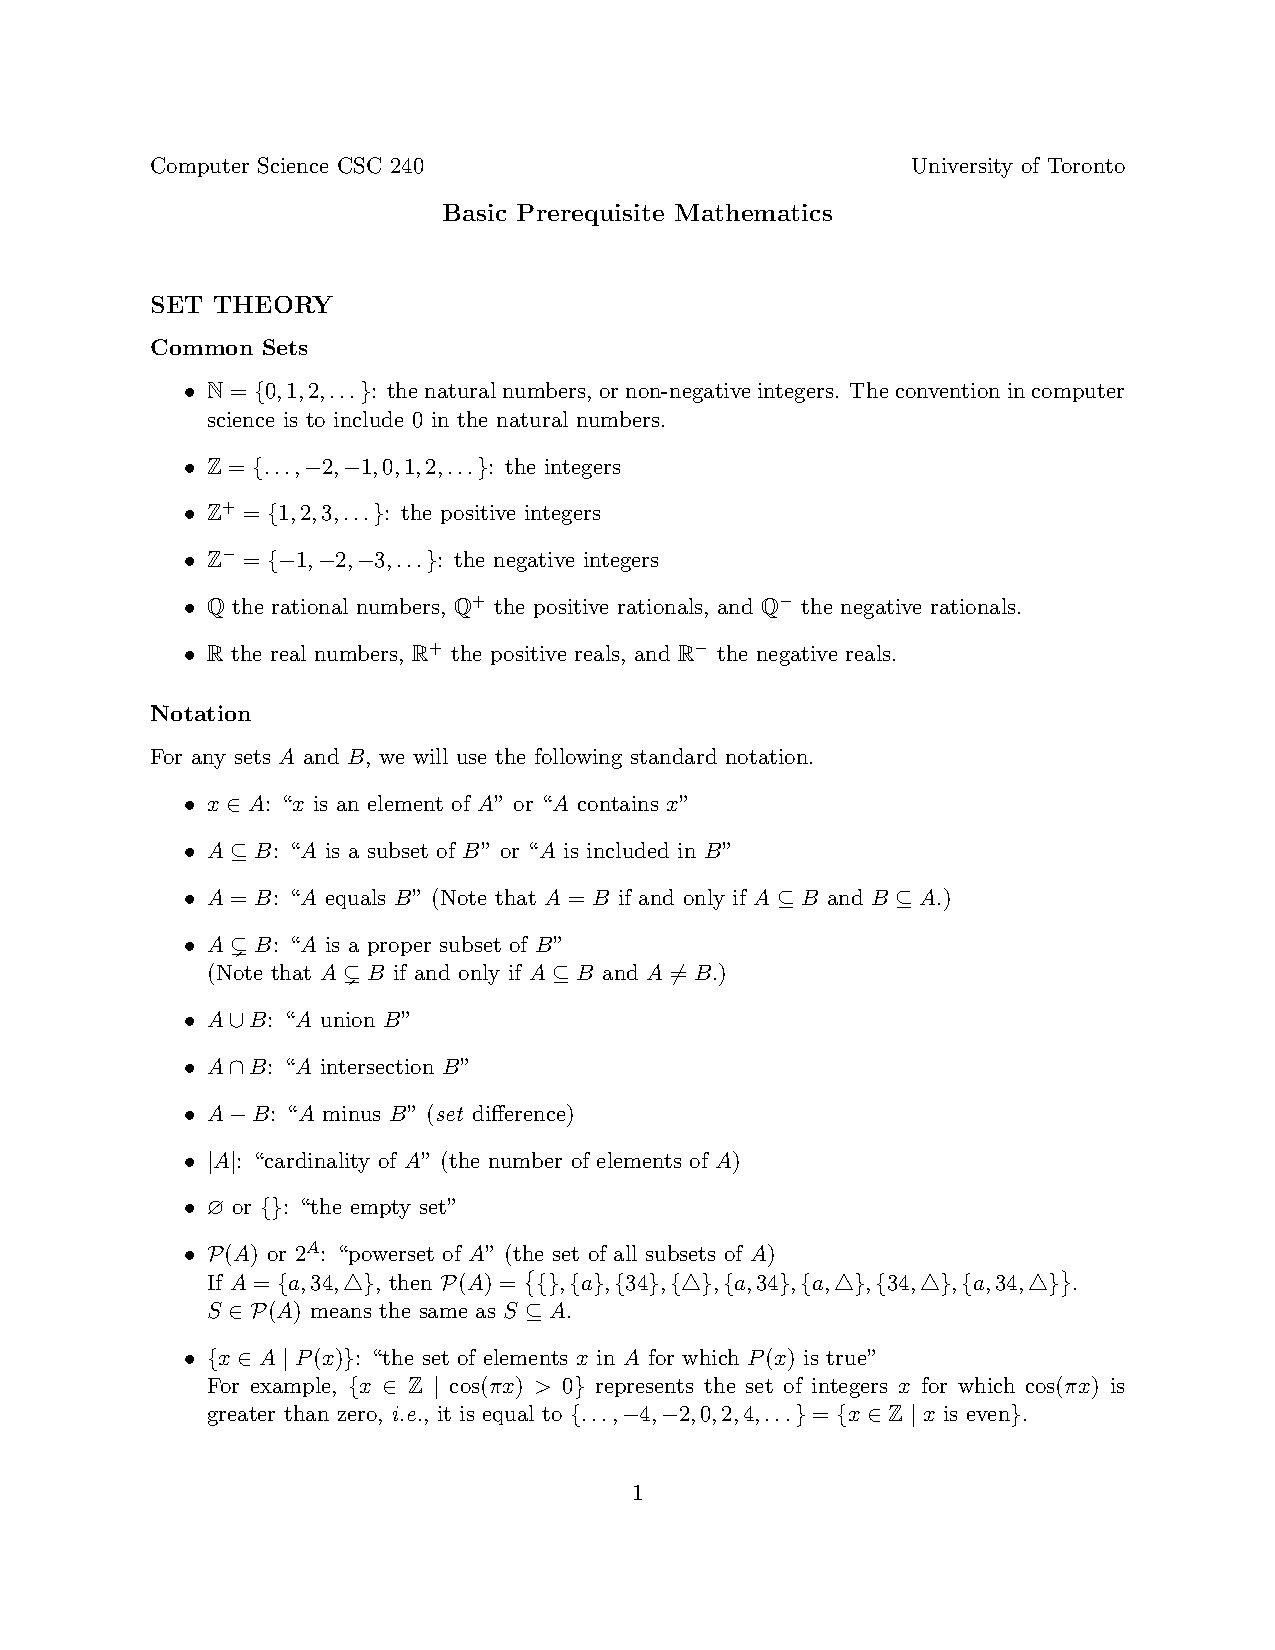
\includepdf[pages=-]{appendix/basicMath.pdf}

\chapter*{Proof Templates}
\addcontentsline{toc}{chapter}{\textcolor{ocre}{Proof Templates}}
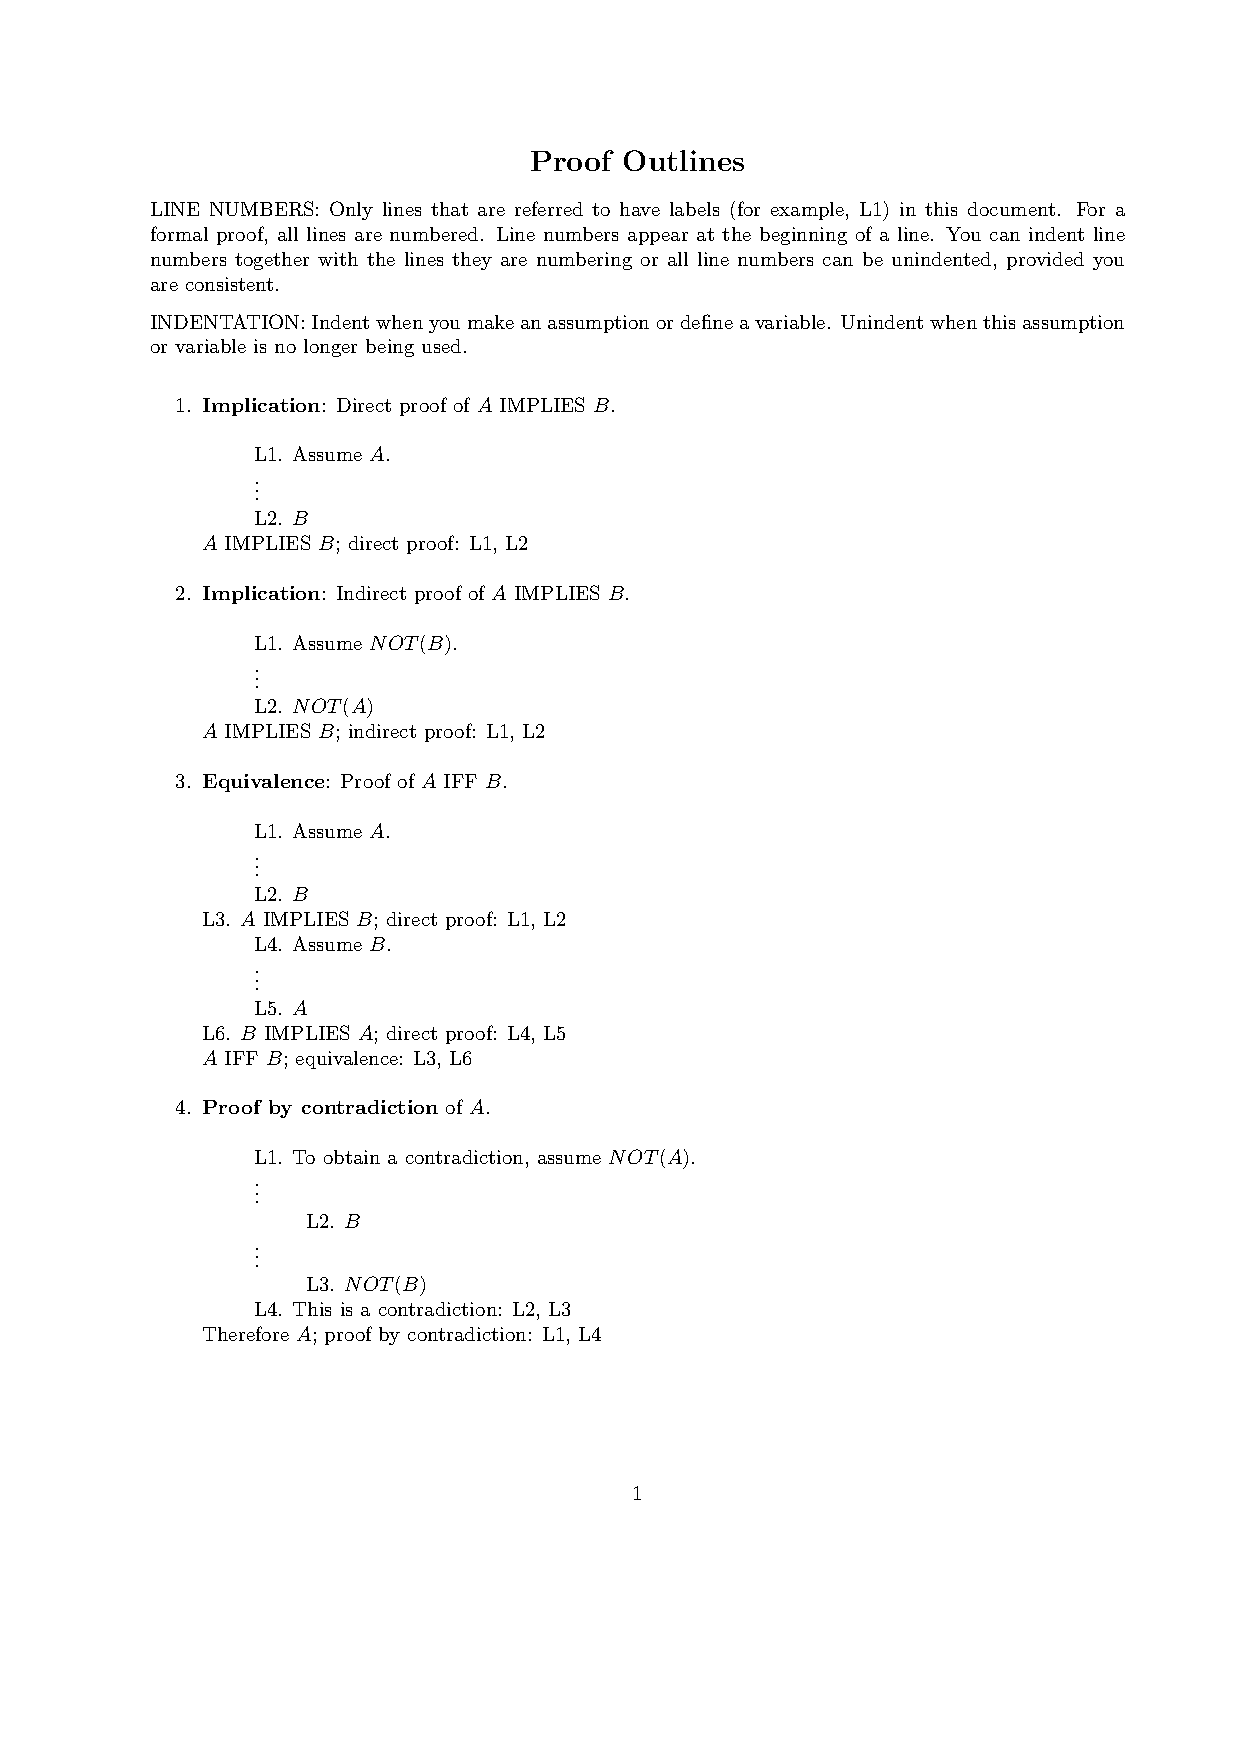
\includepdf[pages=-]{appendix/proofOutlines.pdf}

%----------------------------------------------------------------------------------------
%	INDEX
%----------------------------------------------------------------------------------------

\chapter*{Index}
\renewcommand{\leftmark}{\sffamily\bfseries Index}
\renewcommand{\rightmark}{\sffamily\bfseries Index}
%\cleardoublepage % Make sure the index starts on an odd (right side) page
\setlength{\columnsep}{0.75cm} % Space between the 2 columns of the index
\addcontentsline{toc}{chapter}{\textcolor{ocre}{Index}} % Add an Index heading to the table of contents

\printindex % Output the index

%------------------------------------------------
%   BIBLIOGRAPHY ENTRIES
%------------------------------------------------
\chapter*{Bibliography}
\renewcommand{\leftmark}{\sffamily\bfseries Bibliography}
\renewcommand{\rightmark}{\sffamily\bfseries Bibliography}
\addcontentsline{toc}{chapter}{\textcolor{ocre}{Bibliography}} % Add a Bibliography heading to the table of contents

\section*{Courses}
\addcontentsline{toc}{section}{Courses}
\printbibliography[heading=bibempty,type=misc]

\section*{Books}
\addcontentsline{toc}{section}{Books}
\printbibliography[heading=bibempty,type=book]

\section*{Journal Articles}
\addcontentsline{toc}{section}{Journal Articles}
\printbibliography[heading=bibempty,type=article]

\newpage

%------------------------------------------------
%   TUTORIALS
%------------------------------------------------

%----------------------------------------------------------------------------------------

\end{document}
